%%%%%%%%%%%%%%%%%%%%%%%%%%%%%%%%%%%%%%%%%%%%%%%%%%%%%%%%%%%%%%%%%%%%%%%%%%%%%%%%
%                         FORMATO DE TESIS UMSNH                               %
%%%%%%%%%%%%%%%%%%%%%%%%%%%%%%%%%%%%%%%%%%%%%%%%%%%%%%%%%%%%%%%%%%%%%%%%%%%%%%%%
% based on Harish Bhanderi's PhD/MPhil template, then Uni Cambridge
% http://www-h.eng.cam.ac.uk/help/tpl/textprocessing/ThesisStyle/
% corrected and extended in 2007 by Jakob Suckale, then MPI-iCBG PhD programme
% and made available through OpenWetWare.org - the free biology wiki

%                     Under GNU License v3
% Adaptado para UNAM: @Tepexic
% ADAPTADO PARA UMSNH:  @arturolp

\documentclass[twoside,11pt]{Latex/Classes/PhDthesisPSnPDF} % "thesisUMSNH" para formato de la UMSNH
%         PUEDEN INCLUIR EN ESTE ESPACIO LOS PAQUETES EXTRA, O BIEN, EN EL ARCHIVO "PhDthesisPSnPDF.cls" EN "./Latex/Classes/"


\usepackage[spanish,es-tabla]{babel}
\usepackage[left=2.5cm,bottom=4.5cm]{geometry}
\spanishdecimal{.}
\usepackage[utf8]{inputenc}
\usepackage{graphicx}
\usepackage{hyperref} % Para que las ecuaciones referencíen con links
\usepackage{booktabs}
\usepackage{fullpage}
\usepackage{float}
\usepackage{lscape}
\usepackage{parskip}
% Estos paquetes son opcionales y a necesidad de cada quien:
\usepackage{blindtext}                             % Para insertar texto dummy, de ejemplo, pues.
\usepackage{amssymb, amsmath, amsbsy, amsfonts,amssymb}    % ECUACIONES Y SÍMBOLOS MATEMÁTICOS
\usepackage{listings}                    % PERMITE AGREGAR CÓDIGO DE LENGUAJES  DE PROGRAMACIÓN (DOCUMENTACIÓN EN GOOGLE)
\usepackage{mathdots}                    % para el comando \iddots
\usepackage{mathrsfs}                    % para formato de letra en ecuaciones
\usepackage[numbers]{natbib}  % Personalizar la bibliografía a gusto de cada quien
\usepackage[svgnames]{xcolor}
\usepackage[most]{tcolorbox}
\usepackage{algorithm}
\renewcommand{\listalgorithmname}{Lista de Algoritmos}
\usepackage[noend]{algpseudocode}
\usepackage{amsthm}
\usepackage{imakeidx}

\makeatletter
\renewcommand{\ALG@name}{Algoritmo} % Changing the caption name to Spanish
\makeatother


\usetikzlibrary{shadows}

\newcounter{exa}

\tcbset{
  myexample/.style={
    enhanced,
    colback=yellow!10!white,
    colframe=red!50!black,
    fonttitle=\scshape,
    titlerule=0pt,
    title={\refstepcounter{exa}Ejemplo~\theexa.},
    title style={fill=yellow!10!white},
    coltitle=red!50!black,
    drop shadow,
    highlight math style={reset,colback=LightBlue!50!white,colframe=Navy}
  }
}


\newtheorem{definition}{Definición}

\newtheoremstyle{defstyle} % name of the style
  {3pt} % Space above
  {3pt} % Space below
  {} % Body font
  {} % Indent amount
  {\bfseries} % Theorem head font
  {:} % Punctuation after theorem head
  {.5em} % Space after theorem head
  {} % Theorem head spec

\theoremstyle{defstyle}


\newtcolorbox{texample}{myexample}

% * Ejemplo de ejemplo
% \begin{texample}\label{ex:one}
%     \centering
%     \tcbhighmath{\textrm{d}X_{t}=b(t,X_{t})+\sigma(t,X_{t}) \textrm{d}W_{t}}\quad
%     \begin{tabular}{|c|c|}
%     \hline
%     \textcolor{red!70!black}{W} & \textcolor{Navy}{C} \\
%     \hline
%     $+$ & $-$ \\
%     \hline
%     \end{tabular}
%     \end{texample}
    
% As you can see in Example~\ref{ex:one}, we can create a nice example box with a label.


% Note:
% The \blindtext or \Blindtext commands throughout this template generate dummy text
% to fill the template out. These commands should all be removed when 
% writing thesis content.




% https://github.com/Tepexic/Tesis-UNAM


%%%%%%%%%%%%%%%%%%%%%%%%%%%%%%%%%%%%%%%%%%%%%%%%%%%%%%%%%%%%%%%%%%%%%%%%%%%%%%%%
%                                   DATOS                                      %
%%%%%%%%%%%%%%%%%%%%%%%%%%%%%%%%%%%%%%%%%%%%%%%%%%%%%%%%%%%%%%%%%%%%%%%%%%%%%%%%
\title{Reducción de objetivos en problemas multiobjetivo usando indicadores de calidad.}
\author{Fernando Avitúa Varela} 
\facultad{Instituto de Investigación en Matemáticas Aplicadas y en Sistemas} % Nombre de la facultad/escuela
\escudofacultad{Latex/Classes/Escudos/IIMAS} % Aquí ponen la ruta y nombre del escudo de su facultad, actualmente, la carpeta Latex/Classes/Escudos cuenta con los siguientes escudos:
% "fi_azul" Facultad de ingenieria en color azul
% "fi_negro" Facultad de ingenieria en color negro
% "fc_azul" Facultad de ciencias en color azul
% "fc_negro" Facultad de ciencias en color negro
% "fmed_grande" Facultad de medicina UMSNH
% Se agradecen sus aportaciones de escudos a jebus.velazquez@gmail.com

\degree{Licenciado en Ciencia de Datos}       % Carrera
\director{Dr. Carlos Ignacio Hernández Castellanos}                 % Director de tesis
%\tutor{Nombre  Tutor }                    % Tutor de tesis, si aplica
\degreedate{2023}                          % Año de la fecha del examen
\lugar{Ciudad Universitaria, CDMX}         % Lugar

%\portadafalse                              % Portada en NEGRO, descomentar y comentar la línea siguiente si se quiere utilizar
\portadatrue                                % Portada en COLOR



%% Opciones del posgrado (descomentar si las necesitan)
	%\posgradotrue                                                    
	%\programa{programa de maestría y doctorado en ingeniería}
	%\campo{Ingeniería Eléctrica - Control}
	%% En caso de que haya comité tutor
	%\comitetrue
	%\ctutoruno{Dr. Emmet L. Brown}
	%\ctutordos{Dr. El Doctor}
%% Datos del jurado                             
	%\presidente{Dr. 1}
	%\secretario{Dr. 2}
	%\vocal{Dr. 3}
	%\supuno{Dr. 4}
	%\supdos{Dr. 5}
	%\institucion{el Instituto de Ingeniería, UNAM}

\keywords{optimización,multiobjetivo,indicadores,calidad,PFI-EMOA}            % Palablas clave para los metadatos del PDF
% \subject{tema_1,tema_2}                     % Tema para metadatos del PDF  

%%%%%%%%%%%%%%%%%%%%%%%%%%%%%%%%%%%%%%%%%%%%%%%%%%%%%
%                   PORTADA                         %
%%%%%%%%%%%%%%%%%%%%%%%%%%%%%%%%%%%%%%%%%%%%%%%%%%%%%
\begin{document}

% This file contains macros that can be called up from connected TeX files
% It helps to summarise repeated code, e.g. figure insertion (see below).

%%%%%%%%%%%%%%%%%%%%%%%%%%%%%%%%%%%%%%%%%%%%%%
%            Colores de la UNAM              %
%%%%%%%%%%%%%%%%%%%%%%%%%%%%%%%%%%%%%%%%%%%%%%
% Para UNAN: Azul Pantone 655C-->(0,3,84) RGB
% Para UMSNH: PANTONE Blue 072 C
\definecolor{Azul}{RGB}{0,3,84}

% Para UNAM: Oro PANTONE 871C-->(137,118,75) RGB
% Para UMNSH: PANTONE 110 C
\definecolor{Oro}{RGB}{137,118,75}


%%%%%%%%%%%%%%%%%%%%%%%%%%%%%%%%%%%%%%%%%%%%%%
%            Comandos para líneas            %
%%%%%%%%%%%%%%%%%%%%%%%%%%%%%%%%%%%%%%%%%%%%%%
%Se define un comando \colorvrule para hacer líneas verticales de color con 3 argumentos: color, ancho, alto
\newcommand{\colorvrule}[3]{
\begingroup\color{#1}\vrule width#2 height#3
\endgroup}

%Se define un comando \colorhrule para hacer líneas horizontales de color con 2 argumentos: color, ancho
\newcommand{\colorhrule}[2]{
\begingroup\color{#1}\hrule height#2
\endgroup}

%%%%%%%%%%%%%%%%%%%%%%%%%%%%%%%%%%%%%%%%%%%%%%
%          Comando para derivadas            %
%%%%%%%%%%%%%%%%%%%%%%%%%%%%%%%%%%%%%%%%%%%%%%
\newcommand{\derivada}[3][]{\ensuremath{\dfrac{\mbox{d}^{#1}#2}{\mbox{d}#3^{#1}}}} 
%primer argumento(opcional): orden de la derivada
%segundo argumento: función a derivar
%tercer argumento: variable respecto a la que se deriva


%%%%%%%%%%%%%%%%%%%%%%%%%%%%%%%%%%%%%%%%%%%%%%
%       Comando para la exponencial          %
%%%%%%%%%%%%%%%%%%%%%%%%%%%%%%%%%%%%%%%%%%%%%%
\newcommand{\e}[1][]{\ensuremath{\mbox{e}^{#1}}}
%primer argumento(opcional): exponente de la exponencial




% insert a centered figure with caption and description
% parameters 1:filename, 2:title, 3:description and label
\newcommand{\figuremacro}[3]{
	\begin{figure}[htbp]
		\centering
		\includegraphics[width=1\textwidth]{#1}
		\caption[#2]{\textbf{#2} - #3}
		\label{condicion}
	\end{figure}
}

% insert a centered figure with caption and description AND WIDTH
% parameters 1:filename, 2:title, 3:description and label, 4: textwidth
% textwidth 1 means as text, 0.5 means half the width of the text
\newcommand{\figuremacroW}[4]{
	\begin{figure}[htbp]
		\centering
		\includegraphics[width=#4\textwidth]{#1}
		\caption[#2]{\textbf{#2} - #3}
		\label{#1}
	\end{figure}
}

% inserts a figure with wrapped around text; only suitable for NARROW figs
% o is for outside on a double paged document; others: l, r, i(inside)
% text and figure will each be half of the document width
% note: long captions often crash with adjacent content; take care
% in general: above 2 macro produce more reliable layout
\newcommand{\figuremacroN}[3]{
	\begin{wrapfigure}{o}{0.5\textwidth}
		\centering
		\includegraphics[width=0.48\textwidth]{#1}
		\caption[#2]{{\small\textbf{#2} - #3}}
		\label{#1}
	\end{wrapfigure}
}

% predefined commands by Harish
\newcommand{\PdfPsText}[2]{
  \ifpdf
     #1
  \else
     #2
  \fi
}

\newcommand{\IncludeGraphicsH}[3]{
  \PdfPsText{\includegraphics[height=#2]{#1}}{\includegraphics[bb = #3, height=#2]{#1}}
}

\newcommand{\IncludeGraphicsW}[3]{
  \PdfPsText{\includegraphics[width=#2]{#1}}{\includegraphics[bb = #3, width=#2]{#1}}
}

\newcommand{\InsertFig}[3]{
  \begin{figure}[!htbp]
    \begin{center}
      \leavevmode
      #1
      \caption{#2}
      \label{#3}
    \end{center}
  \end{figure}
}







%%% Local Variables:
%%% mode: latex
%%% TeX-master: "~/Documents/LaTeX/CUEDThesisPSnPDF/thesis"
%%% End:
           % Archivo con funciones útiles

\maketitle									% Se redefinió este comando en el archivo de la clase para generar automáticamente la portada a partir de los datos

%%%%%%%%%%%%%%%%%%%%%%%%%%%%%%%%%%%%%%%%%%%%%%%%%%%%%
%                  PRÓLOGO                          %
%%%%%%%%%%%%%%%%%%%%%%%%%%%%%%%%%%%%%%%%%%%%%%%%%%%%%
\frontmatter
% \begin{dedication}

\blindtext

\end{dedication}
       % Comentar línea si no se usa
% %\chapter*{}
%\pagenumbering{Roman}

\begin{acknowledgements}

\blindtext

\end{acknowledgements}




   % Comentar línea si no se usa 
% % ******************************* Thesis Declaration ********************************

\begin{declaration}

Por la presente declaro que, salvo cuando se haga referencia específica al trabajo de otras personas, el contenido de esta tesis es original y no se ha presentado total o parcialmente para su consideración para cualquier otro título o grado en esta o cualquier otra Universidad. Esta tesis es resultado de mi propio trabajo y no incluye nada que sea el resultado de algún trabajo realizado en colaboración, salvo que se indique específicamente en el texto. 
% Author and date will be inserted automatically from thesis.tex


\end{declaration}
           % Comentar línea si no se usa

% Thesis Abstract -----------------------------------------------------


%\begin{abstractslong}    %uncommenting this line, gives a different abstract heading
\begin{abstracts}        %this creates the heading for the abstract page

% This is where you write your abstract ...
% \blindtext

La optimización multiobjetivo es una rama de las matemáticas aplicadas, con orígenes que se remontan al siglo XIX. Este campo se destaca por abordar preguntas complejas relacionadas con buscar una decisión óptima en un problema con varias características a optimizar. Esta complejidad en el planteamiento del problema llevó al desarrollo del concepto del frente de Pareto. Este concepto subraya que la situación ideal en un problema multiobjetivo no será necesariamente donde todos los  objetivos se optimizan individualmente, sino más bien un conjunto de soluciones en las que no se pueda encontrar una solución que sea mejor que las demás en todos los objetivos.

La investigación de este trabajo se enfoca en el uso de algoritmos evolutivos para la optimización multiobjetivo, conocidos como EMOAs. Estos algoritmos se inspiran en los procesos evolutivos de la naturaleza para producir soluciones adaptables y diversas, operando sin necesidad de conocer la forma exacta de la función objetivo. La tesis se centra en estudiar de manera estadística diferentes hiperparámetros dentro de un EMOA existente, el algoritmo conocido como PFI-EMOA. El objetivo del trabajo es primero demostrar y luego comprender por qué ciertos parámetros resultan más eficaces que otros.

El estudio incluye una serie de experimentos utilizando combinaciones de los indicadores IGD+, R2 y Energía-S de Riesz en una variedad de problemas de prueba. A través de comparaciones estadísticas, se evaluó la existencia y magnitud de diferencias significativas en el rendimiento del algoritmo. Se buscó determinar si ciertas combinaciones de pesos eran consistentemente más efectivas que otras, o si los resultados variaban según el problema específico.

Mirando hacia el futuro, la tesis plantea preguntas para investigaciones subsecuentes. Una de ellas es qué tipos de problemas favorecen ciertas combinaciones de indicadores y la posibilidad de modificar dinámicamente los pesos de los indicadores en respuesta a los resultados intermedios del algoritmo. Esto permitiría una búsqueda más eficiente, inclinándose hacia el indicador de convergencia o diversidad según sea necesario.

\end{abstracts}
%\end{abstractlongs}


% ----------------------------------------------------------------------                   % Comentar línea si no se usa

%%%%%%%%%%%%%%%%%%%%%%%%%%%%%%%%%%%%%%%%%%%%%%%%%%%%%
%                   ÍNDICES                         %
%%%%%%%%%%%%%%%%%%%%%%%%%%%%%%%%%%%%%%%%%%%%%%%%%%%%%
%Esta Sección genera el índice
\setcounter{secnumdepth}{3} % organisational level that receives a numbers
\setcounter{tocdepth}{3}    % print table of contents for level 3
\tableofcontents            % Genera el índice 
%: ----------------------- list of figures/tables ------------------------
\listoffigures              % Genera el ínidce de Figuras, comentar línea si no se usa
\listoftables               % Genera índice de Tablas, comentar línea si no se usa
\listofalgorithms



%%%%%%%%%%%%%%%%%%%%%%%%%%%%%%%%%%%%%%%%%%%%%%%%%%%%%
%                   CONTENIDO                       %
%%%%%%%%%%%%%%%%%%%%%%%%%%%%%%%%%%%%%%%%%%%%%%%%%%%%%
% the main text starts here with the introduction, 1st chapter,...
\mainmatter
\def\baselinestretch{1.5}                   % Interlineado de 1.5


\chapter{Introducción}


La optimización multiobjetivo es una disciplina dentro de las matemáticas aplicadas, con sus orígenes remontándose al siglo XIX. Esta área se destaca por abordar la compleja pregunta formulada por un economista de esa época, quien se interrogaba sobre la forma óptima en que podría vivir un grupo de personas. Esta pregunta llevó al desarrollo de una de las definiciones más cruciales en este campo: \textbf{el frente de Pareto}. La idea central del frente de Pareto es que la situación ideal en un sistema de recursos limitados no es aquella donde todos maximizan sus recursos, sino más bien aquella en la que ninguna mejora individual es posible sin perjudicar a otro. 

En el intento de comprender y abordar las complejidades del mundo, a menudo tendemos a simplificar los problemas, buscando respuestas concretas en las que se optimiza un solo objetivo aunque esta manera de verlo no caracterice de manera fiel a los problemas. El campo de la optimización multiobjetivo se desvía de esta tendencia, cambiando su enfoque a estudiar problemas con múltiples dimensiones en sus espacios de objetivos. Estos problemas ya no requieren no soluciones puntuales, sino conjuntos de soluciones. Dichos conjuntos de soluciones son tales que no existe una forma en la que todos los aspectos del problema puedan ser mejorados simultáneamente. Con el tiempo, la relevancia y aplicabilidad de la optimización multiobjetivo han crecido mucho, encontrando uso en áreas tan diversas como la bioinformática \cite{handlMultiobjectiveOptimizationBioinformatics2007}, redes inalámbricas \cite{gunjanReviewMultiobjectiveOptimization2023}, procesamiento del lenguaje natural (NLP) \cite{sainiMultiobjectiveOptimizationTechniques2021}, procesamiento de imágenes \cite{aslamComprehensiveSurveyOptimization2020}, y en los campos de la astronomía y astrofísica \cite{mullerUsingMultiobjectiveOptimization2023}. A diferencia de los problemas de un solo objetivo, donde técnicas como el descenso del gradiente han demostrado ser exitosas en aprendizaje automático y redes neuronales, los problemas multiobjetivo presentan una complejidad adicional que exploraremos a lo largo de este trabajo.


Al abordar problemas multiobjetivo, nos encontramos con desafíos únicos. Uno de los más significativos es la imposibilidad de establecer un orden total en un espacio con múltiples objetivos.  Este obstáculo se ve exacerbado por la \emph{maldición de la dimensionalidad}, un fenómeno bien conocido en el campo de la computación, donde el aumento de las dimensiones de un problema no resulta en una simple generalización de un problema unidimensional. La complejidad aumenta de manera no trivial con cada dimensión adicional, lo que hace que muchas técnicas de optimización convencionales sean inadecuadas para estos problemas.

Frente a esta complejidad, un enfoque que ha demostrado ser especialmente valioso es el uso de \textbf{algoritmos evolutivos} \cite{coelloEvolutionaryAlgorithmsSolving}. Inspirados en los procesos evolutivos de la naturaleza, estos algoritmos buscan encontrar estrategias exitosas para producir soluciones altamente adaptables y diversas. Estos algoritmos, conocidos como Algoritmos Evolutivos para Optimización Multiobjetivo (MOEAs), se caracterizan por su capacidad para generar progresivamente una población más apta a través de un método iterativo. Una ventaja clave de los MOEAs es su habilidad para operar sin necesidad de conocer la forma cerrada de las funciones objetivo, una situación común en los problemas multiobjetivo. En este trabajo, exploraremos en profundidad el potencial y la aplicación de los algoritmos evolutivos en la resolución de problemas multiobjetivos complejos.

El campo de los Algoritmos Evolutivos para Optimización Multiobjetivo (MOEAs) es vasto y diverso, con varias clasificaciones para diferentes enfoques en la aproximación a los Problemas de Optimización Multiobjetivo (MOP). Un enfoque particularmente interesante es el de los algoritmos basados en \textbf{indicadores de calidad}, que se detallarán en la Sección \ref{sec:SMS-EMOA}. Estos algoritmos utilizan características específicas, o indicadores, de las soluciones propuestas para guiar el proceso de búsqueda evolutiva con el fin de encontrar la mejor representación del frente de Pareto posible. Una caracterización que resultará útil de estos indicadores es en la manera en la que caracterizan el conjunto de soluciones. En particular, nos concentraremos en dos categorías importantes que son los indicadores de convergencia y los de indicadores de diversidad. Los indicadores de convergencia evalúan qué tan cerca se encuentra el conjunto de soluciones del frente de Pareto, o de una aproximación de este. Por otro lado, los indicadores de diversidad examinan la uniformidad y el espaciamiento entre las soluciones. Mejorando ambos tipos de indicadores—uno de convergencia y otro de diversidad—se logra una representación más fidedigna al frente de Pareto (ver Figura \ref{fig:aproximacion}).

A pesar de la existencia de numerosos esfuerzos dirigidos a resolver problemas multiobjetivo mediante el diseño de nuevos algoritmos evolutivos, este trabajo se centra en un enfoque diferente. En lugar de desarrollar un nuevo método, nos dedicaremos al estudio exhaustivo de diferentes configuraciones de un algoritmo evolutivo ya establecido; el EMOA llamado PFI-EMOA (Pareto Front Invariant-EMOA) \cite{PFI}. Este algoritmo realiza una combinación ponderada entre un indicador de convergencia conocido como IGD+ \cite{IGD} y un indicador de diversidad denominado Energía S de Riez \cite{sEnergy} para guiar la búsqueda en el espacio de estados y obtener conjuntos de soluciones que no tengan problemas encontrando frentes de Pareto con los que otros algoritmos han tenido dificultades. Las diferentes configuraciones que probaremos corresponden a cambiar el peso con el que se combinan estos indicadores en el algoritmo. 
    
Dado lo anterior, podemos resumir las intenciones de este trabajo en las siguientes preguntas:

\begin{itemize}
    \item La primera y más fundamental es: \textbf{¿Existe una diferencia en el desempeño del algoritmo PFI-EMOA al variar la combinación de IGD+ y S-Energy?}
    La respuesta a esta pregunta no es obvia, ya que podría ser que la combinación específica de indicadores no importe siempre y cuando se usen ambos para atacar el problema. Para probar este punto se usaron un conjunto de problemas de prueba que ya son estándar en la literatura de MOPs para vigilar el desempeño en cada uno de ellos. 
    \\Encontramos que si existe una diferencia significativa para la mayoría de los problemas. Es decir, si importa si escogemos darle mayor contribución a un operador de convergencia que a alguno de calidad
    \item Después sigue la pregunta natural: \textbf{¿Qué combinación de pesos es mejor para cada familia de problemas?}
    De igual manera esta respuesta no será obvia. Habrá problemas que por su forma requieran más exploración del espacio de estados y esto puede significar que necesitan tener una contribución mayor del indicador de diversidad. \\
    Para cada problema esto será distinto, sin embargo, encontramos resultados generales para agrupaciones útiles como por el número de objetivos y por el tipo de indicadores de calidad. De forma general encontramos que darle más peso a IGD+ resulta ser mejor para obtener buenos resultados de convergencia y viceversa para S-Energy, teniendo el caso excepcional del mismo S-Energy. Es decir, el intentar optimizar este indicador durante la búsqueda, no asegura que existan soluciones que lo maximicen.
    \item Como también variamos la combinación de indicadores con respecto a PFI-EMOA la siguiente pregunta es: \textbf{¿Qué sucede cuando cambiamos el indicador de IGD+ a otro indicador de convergencia?}
    En este trabajo, además de estudiar el efecto de IGD+ a detalle, sustituimos el indicador de convergencia R2 \cite{R2} que se explica en la sección \ref{sec:R2}. Aunque ambos indicadores se preocupan principalmente con la convergencia del conjunto de soluciones, se definen de manera distinta, por lo que no tenemos garantizado obtener el mismo resultado al usar uno o el otro.\\
    Encontramos que la decisión de darle diferentes pesos a la combinación de indicadores cuando está presente el IGD+ es mucho más importante que la del R2. Teniendo este último muy pocas situaciones donde existe una diferencia significativa entre una y otra combinación de pesos.
   
\end{itemize}


Para abordar las preguntas planteadas, llevamos a cabo un protocolo de experimentación empírico, utilizando distintas combinaciones de los indicadores IGD+ y S-Energy. Aquí surge la pregunta de cómo vamos a evaluar el desempeño de cada una de las diferentes combinaciones para esto necesitamos evaluar los algoritmos bajo las mismas circunstancias. Así, por cada diferente configuración de hiperparámetros (pesos de los indicadores de convergencia y distribución) primero tomaremos un conjunto de problemas prueba (CITE problemas prueba) con diferente número de objetivos (como se puede ver en la tabla \ref{Tabla:problema_prueba}) y después evaluar la solución obtenida usando indicadores de calidad que se explicarán en la sección \ref{sec:QIs} e incluyen: Hipervolumen \ref{sec:HV}, Distancia Generacional Invertida IGD \ref{sec:IGD}, Epsilon +\ref{sec:Epsilonp}, Diversidad de Solow-Polasky \ref{sec:SPD}, R2 \ref{sec:R2} y los dos que se usaron para guiar la búsqueda, es decir, IGD+ y Energía S de Riesz. Es decir, se obtiene una solución guiada por una combinación específica del indicador de convergencia y distribución y luego se evalúa usando otro indicador. Estas evaluaciones se realizan para poblaciones inicializadas de acuerdo a 10 semillas distintas. Así se obtienen 10 resultados por cada uno de los indicadores de evaluación y podemos compararlos entre sí usando pruebas estadísticas para decidir si una configuración de hiperparámetros es mejor a otra.
% TODO: Referencia de problemas prueba

El objetivo del trabajo es determinar si ciertas combinaciones de pesos son consistentemente más efectivas que otras y si estos resultados varían según el problema específico. Inicialmente, analizamos el número de problemas en los que la elección de pesos tenía un impacto relevante. Posteriormente, nos centramos en identificar, para cada indicador y número de objetivos, las combinaciones de pesos que ofrecían un mejor rendimiento.

Este trabajo está organizado de la siguiente manera para facilitar una comprensión integral del estudio realizado:

\begin{itemize}
    \item \textbf{Capítulo 1: Introducción a los Problemas Multiobjetivo.} Este capítulo proporciona una introducción detallada a los problemas multiobjetivo, estableciendo el lenguaje y los conceptos clave que serán utilizados a lo largo de la tesis.
    \item \textbf{Capítulo 2: Algoritmos Evolutivos y su Aplicación.} Aquí definimos qué son los algoritmos evolutivos y cómo se aplican en la solución de problemas multiobjetivo. Se incluye una descripción de varios algoritmos evolutivos multiobjetivo exitosos, así como la posición del algoritmo que es el foco de este trabajo dentro de este contexto. También se presentan las definiciones de todos los indicadores de calidad que emplearemos, junto con la metodología para comparar los resultados de los algoritmos, utilizando pruebas estadísticas como Kruskal-Wallis y Wilcoxon.
    \item \textbf{Capítulo 3: Diseño del Procedimiento Experimental.} En este capítulo, detallamos cómo se diseñó el procedimiento experimental, incluyendo la selección de algoritmos, las combinaciones de pesos utilizadas, los problemas de prueba seleccionados y el número de objetivos considerados. Se presentan algunos de los resultados más interesantes que forman la base para la discusión en el siguiente capítulo.
    \item \textbf{Capítulo 4: Discusión de Resultados.} Aquí discutimos los resultados obtenidos, enmarcándolos en el contexto de las preguntas de investigación planteadas anteriormente.
    \item \textbf{Capítulo 5: Conclusiones y Trabajo Futuro.} Finalmente, en el último capítulo, ofrecemos las conclusiones derivadas de nuestra investigación y delineamos posibles direcciones para futuros estudios en este campo.
\end{itemize}





            % ~10 páginas - Explicar el propósito de la tesis

% %%%%%%%%%%%%%%%%%%%%%%%%%%%%%%%%%%%%%%%%%%%%%%%%%%%%%%%%%%%%%%%%%%%%%%%%%
% %           Capítulo 2: MARCO TEÓRICO - REVISIÓN DE LITERATURA
% %%%%%%%%%%%%%%%%%%%%%%%%%%%%%%%%%%%%%%%%%%%%%%%%%%%%%%%%%%%%%%%%%%%%%%%%%

\chapter{Fundamentos Previos}

En este capítulo se da la teoría preliminar necesaria que forma las bases del problema a atacar. Se comienza en la Sección \ref{sec:Dominancia_Pareto} describiendo de manera formal un problema de optimización multiobjetivo, en la siguiente Sección \ref{sec:clasif_MOO} se explica una clasificación breve de algoritmos usados para optimizar problemas multiobjetivo visto desde la perspectiva de la estrategia usada para resolverlo; es decir, cuándo se usan las preferencias del tomador de decisiones para buscar las soluciones. Después, en la Sección \ref{sec:Escalarizaciones}, se explican escalarizaciones comunes, haciendo énfasis en la función aumentada de Tchebycheff que se usará frecuentemente en este trabajo. 
Se concluye el capítulo en la Sección \ref{sec:AE} con una explicación breve de qué son los algoritmos Evolutivos.



\section{Optimización multiobjetivo} \label{sec:MOO}



La \textbf{optimización} es una rama de las matemáticas aplicadas y de la computación, dedicada a encontrar métodos efectivos para realizar tareas específicas. Esto incluye, por ejemplo, optimizar algoritmos o minimizar errores a través de la adecuada configuración de parámetros.

Tradicionalmente, la optimización se ha centrado en \textit{problemas de objetivo único} (SOP por sus siglas en inglés), por su simplicidad y la factibilidad de encontrar soluciones. Sin embargo, la realidad muestra que la mayoría de los problemas son de un carácter \textit{multiobjetivo} (MOP por sus siglas en inglés), dada su complejidad y múltiples metas involucradas.

Atender un problema únicamente desde una perspectiva SOP puede resultar en una simplificación excesiva. El enfoque de MOP permite capturar la complejidad real del problema, ofreciendo una visión más integral y representativa del entorno en el que se desenvuelve.

Definiremos formalmente los componentes de un MOP en la Sección \ref{sec:Dominancia_Pareto}, explorando cómo este enfoque puede proporcionar soluciones más completas y realistas a problemas complejos. Después, en la Sección \ref{sec:clasif_MOO} explicaremos una clasificación de algoritmos multiobjetivo en términos generales. Luego, definiremos escalarizaciones comúnes que también usaremos para definir el algoritmo usado en este trabajo en la Sección \ref{sec:Escalarizaciones}.

Concluiremos el capítulo en la Sección \ref{sec:AE}, explicando los algoritmos evolutivos que usaremos en este trabajo para encontrar encontrar una solución a un MOP (los algoritmos son llamados MOEAs por sus siglas en inglés). 

Para tratar este problema desde una aplicación específica a ciencia de datos tomaremos el siguiente ejemplo de selección de características en un problema de clasificación:

\begin{texample} \label{ex:Selecc}
    Dado un conjunto de datos con $n$ columnas y un algoritmo de k-medias con dos componentes, etiqueta en una de dos clases (0 o 1). El problema de selección de características consiste en encontrar el menor número de columnas posibles tal que el error de clasificación sea mínimo.
    
    Así, tenemos que minimizar dos objetivos: el número de características y el error de clasificación, volviendo a esto un problema de optimización biobjetivo. 
\end{texample}


\subsection{Elementos de un problema multiobjetivo: definición matemática} \label{sec:Dominancia_Pareto}

Un problema de optimización multiobjetivo busca encontrar, dadas unas funciones y restricciones, el conjunto de puntos que minimicen dichas funciones bajo estas restricciones. Puede ser caracterizado de manera más formal por las siguientes definiciones, que son ilustradas en la Figura \ref{fig:dec_obj}  \footnote{Imagen tomada de \cite{coelloEvolutionaryAlgorithmsSolving}}. 

\begin{itemize}
    \item \textbf{Región de decisión o factible}, $Q\subseteq \mathbb{R}^n$; corresponde a la región que cumple restricciones $g,f$ que se explican en la siguiente viñeta. 
    
    $$ Q=\left\{x\in \mathbb{R}^n|g_i(x)\leq 0, h_j(x)=0 , 0\leq i \leq n, 0\leq j \leq n,\right\}.$$ 

    La región factible es donde cambian las variables de entrada para intentar optimizar los objetivos. Las funciones que aparecen como condiciones extra se explican en la siguiente viñeta.\\ En el Ejemplo \ref{ex:Selecc} de selección de características  el espacio factible sería una máscara binaria sobre las columnas que usamos (con un 1) y las que no (con un 0). De modo que el espacio está dado por todos los $x\in Q$ tales que  $Q=\{0,1\}^n$.
    \item \textbf{Restricciones} sobre el dominio que se pueden escribir como $J$ restricciones de \textbf{igualdad} e $I$ de \textbf{desigualdad} mediante la siguiente ecuación  
    \begin{align*}
        g_i(x)\leq 0, \ \ i\in\{1,\ldots,I\},\\  h_j(x)=0 ,\ \ j\in{1,\ldots,J}.
    \end{align*} 
    \item Las $m$ \textbf{funciones objetivo} que buscaremos minimizar a través del siguiente mapeo$$ F=(f_0,\ldots,f_{m-1}):Q\rightarrow \mathbb{R}^m. $$
    \item \textbf{Espacio de objetivos}, la imagen de la región factible a través de las funciones objetivo 
     $$F(Q)=\{F(x) | x \in Q\}.$$
     
    Es donde se puede interpretar o evaluar el desempeño del algoritmo. En el Ejemplo \ref{ex:Selecc} tenemos dos objetivos, el primer objetivo $f_0$ que mide el tamaño del conjunto, es decir, las características usadas. El segundo objetivo $f_1$ es el error de clasificación del modelo de modo que conjuntamente viven en $(f_0(x),f_1(x))\in \mathbb{R}^2$.
    
\end{itemize}

\begin{figure}[H]
    \centering
    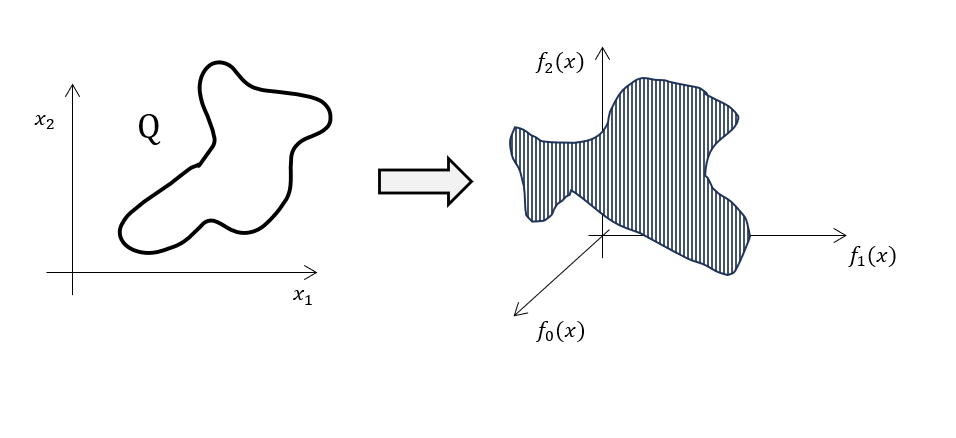
\includegraphics[width=\textwidth]{Figuras/obj_dec.png}
    \caption[Ilustración de un MOP]{Ilustración de un MOP con el espacio factible y el de objetivos. }
    \label{fig:dec_obj}
\end{figure}

Con estos elementos, la finalidad de resolver un problema de optimización multiobjetivo es encontrar el conjunto de vectores en la región factible tal que minimice cada uno de ellos, es decir

\begin{equation} \label{eq:MOO}
    \min_{x\in Q} \{F(x)\}.
\end{equation}

En nuestro Ejemplo \ref{ex:Selecc} buscamos encontrar el vector binario de características tal que minimice tanto el número de columnas usadas por el modelo, así como el error de clasificación. 

Esta definición puede ser fácilmente adaptada al caso donde intentamos maximizar algunos objetivos en vez de minimizarlos. Podemos convertir una objetivo de maximización en uno de minimización haciendo una reflexión en esa dirección; es decir, si el objetivo $i$ se maximizara, podemos obtener un problema de minimización al hacer la siguiente transformación $f_i \rightarrow -f_i$. 

La Ecuación \eqref{eq:MOO} no tiene porque tener solución única. Para convencernos de esto, basta ver la Figura \ref{fig:pareto} y pensar en el caso en el que tenemos dos vectores $x_1, x_2$ tales que $P_1=(f_0(x_1),f_1(x_1)), P_2=(f_0(x_2),f_1(x_2))$. En este caso como podemos ver en la Figura \ref{fig:pareto} $f_0(x_1)< f_0(x_2)$, pero $f_1(x_1) > f_1(x_2)$; es decir, $x_1$ es menor en el primer objetivo que $x_2$, sin embargo, $x_2$ tiene menor segundo objetivo que $x_1$. Así, se vuelve evidente que la meta de la optimización multiobjetivo no será encontrar un punto sino un conjunto de puntos tales que ninguno sea mejor que otro en ambos objetivos.

\begin{figure}[H]
    \centering
    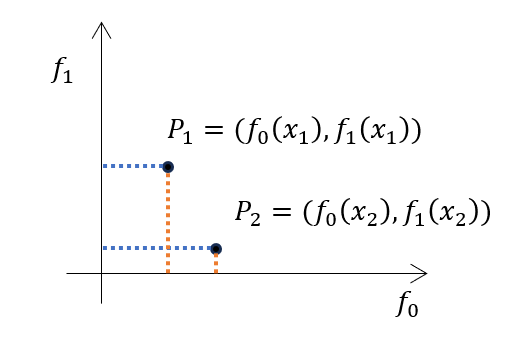
\includegraphics[scale=.5]{Figuras/pareto.png}
    \caption[Vectores en el espacio de objetivos]{Vectores en el espacio de objetivos. .}
    \label{fig:pareto}
\end{figure}


Misma que se puede formular con diferentes niveles cada vez más estrictos de qué significa que un punto domine a otro. Las listamos a continuación:

Para comprender el objetivo de los algoritmos multiobjetivo, es útil recurrir a una analogía social propuesta por Pareto en 1927\footnote{Esta perspectiva se enfoca en el punto de vista \emph{a posteriori}, que se explorará más adelante en la Sección \ref{sec:clasif_MOO}. En otras palabras, tras identificar soluciones para un problema, seleccionamos aquellas que mejor se ajusten a nuestros objetivos.}. Imaginemos una población de $N$ individuos y nuestro desafío es garantizar un estado donde cada uno alcance el máximo bienestar posible. En una sociedad compleja, cualquier cambio en el bienestar de una persona inevitablemente afecta a los demás. Por ejemplo, aumentar la riqueza de un individuo frecuentemente implica redistribuir recursos de otros. Bajo este contexto, Pareto define el estado ideal como aquel donde ninguna persona puede incrementar su bienestar sin perjudicar a otra. Esto se traduce matemáticamente en la noción de \textbf{optimalidad de Pareto}. A continuación mostraremos diferentes definiciones de optimalidad de Pareto en formas cada vez más estrictas, es decir, cada vez se le pide más a un punto para que se considere "mejor" que otro. 


\subsubsection*{Dominancia de Pareto}

\begin{itemize}
    \item Un vector $x\in Q$ es \textbf{preferido} a otro vector $y\in Q$, denotado por $x<_p y \, \, $ si $\, x_i <y_i, \forall i$. De manera análoga se define uno que es menor o igual, denotado por $x\leq_p y$.
    \item Un vector $x\in Q$ \textbf{domina fuertemente} a otro vector $y\in Q$, denotado como $x < y$ con respecto a un MOP como \eqref{eq:MOO}, si sus objetivos son preferidos, es decir, si $F(x) <_p F(y)$.
    \item Un vector $x\in Q$ \textbf{domina} a otro $y\in Q$, denotado $x\prec y$, con respecto a un MOP si $F(x) \leq_p F(y)$ y $F(x)\neq F(y)$, en otro caso se dice que $y\in Q$  es \textbf{no-dominado} por $x\in Q$.
    \item Un vector $x\in Q$ \textbf{domina débilmente} a $y\in Q$, denotado $x\preceq y$ si $F(x)\leq_p F(y)$. Es decir, permitimos el caso donde los puntos sean iguales. 
\end{itemize}

Esto nos da varias nociones de un vector siendo mejor que otro, mientras mejor sea nuestro algoritmo, mayor tenderá hacia la primera definición ya que es más estricta que el resto como podemos ver en la siguiente ecuación

\begin{equation} \label{eq:contencion_def_pareto}
    x <_p  y \implies x \prec y \implies x \preceq y. \nonumber
\end{equation}

\begin{definition}
Diremos que una solución $x\in Q$ es \textbf{óptima de Pareto} si es tal que se cumple
\begin{equation} \label{eq:opt_pareto}
    \nexists \,\, y\in Q \,\, \text{ tal que } y\prec x. \nonumber
\end{equation}

Es decir, no existe ninguna forma de mejorar sin empeorar.
\end{definition}

\begin{definition}
Al conjunto de todos los puntos del espacio factible que son óptimos de Pareto se le conoce como \textbf{Conjunto de Pareto} y a su imagen a través de un MOP, definido en la Ecuación \ref{eq:MOO}, se le conoce como \textbf{Frente de Pareto}. Formalmente se definen como:

El conjunto de Pareto es el conjunto de todas las soluciones óptimas de Pareto, es decir
\begin{equation} \label{eq:pareto_set}
    P=\{x\in Q \, \, \big| \, \, x \text{ Es una solución óptima de Pareto del MOP}\}, \nonumber
\end{equation}

mientras que la imagen del conjunto de Pareto a través de las funciones objetivo es el frente de Pareto 

\begin{equation} \label{eq:pareto_front}
F(P)=\{y\in \mathbb{R}^m \, \, \big| \, \, y=F(x), x \text{ es una solución óptima de Pareto del MOP}\}.    \nonumber
\end{equation}

\end{definition}

El frente de Pareto de un MOP está acotado por dos puntos de referencia: el vector ideal y el vector de Nadir que definimos a continuación y pueden ser visualizados en la Figura \ref{fig:vectores_referencia} (Definiciones y Figura ambas tomadas de \cite{tesis_phd_guillermo}).


\begin{definition} \label{def:Ideal}
    El \textbf{Vector Ideal} vive en el espacio de objetivos y se denota por $z^*\in \mathbb{R}^m$ se define como 
    
    $$z^*_i=\min_{x\in Q}\, f_i(x), \,\, i=1,2,\ldots,m .$$
\end{definition}

\begin{definition} \label{def:Nadir}
    El \textbf{Vector de Nadir} vive en el espacio de objetivos y se denota por $z^{\text{nad}}\in \mathbb{R}^m$ se define como 
    
    $$z^*_i=\max_{x\in \text{PS}}\, f_i(x), \,\, i=1,2,\ldots,m ,$$

    donde $\text{PS}$ es el conjunto de Pareto.
\end{definition}

Estos dos puntos representan la combinación del mejor y el peor de los casos por cada objetivo. Es decir, no es necesario que existan como parte del mapeo del espacio factible. Además a veces es conveniente definir  otro punto que domina al ideal (y por consecuencia al de Nadir) y lo definimos a continuación

\begin{definition} \label{def:utopico}
    Dado el punto ideal $z^*$ y un vector positivo $$\epsilon=(\epsilon_1,\ldots,\epsilon_m) , \epsilon_i>0 \,\, \forall i \in \{1,\ldots,m\},$$
    el \textbf{Vector Utópico} se define como 

    $$ z^{**}=z^*-\epsilon .$$
\end{definition}

\begin{figure}[H]
    \centering
    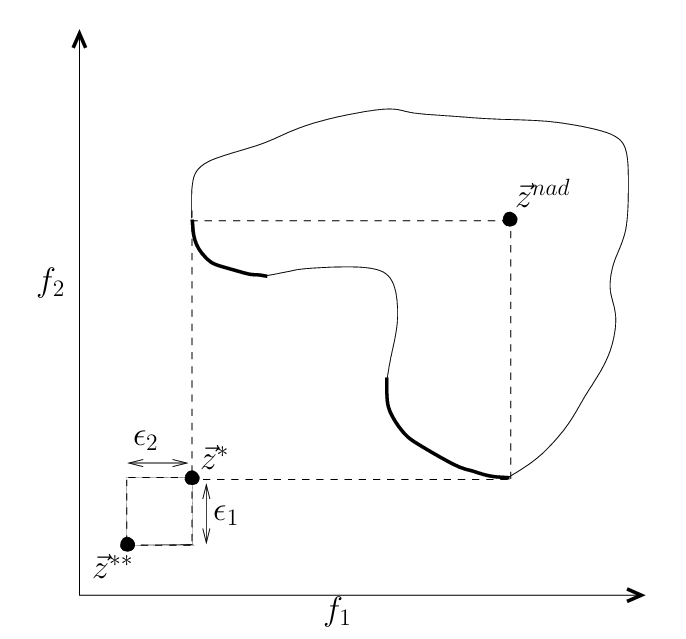
\includegraphics[scale=0.5]{Figuras/nadir_ideal_utopico.png}
    \caption{Vectores de referencia: vector ideal $z^*$, vector de nadir $z^{\text{nadir}}$, vector utópico $z^{**}$.}
    \label{fig:vectores_referencia}
\end{figure}

En general, bajo ciertos supuestos, el frente de Pareto suele formar un espacio de \emph{una} dimensión menor al número de objetivos, aunque esto no es necesario.

\subsection{Clasificación de algoritmos multiobjetivo} \label{sec:clasif_MOO}

Al aproximarse a la solución de un problema multiobjetivo, salen naturalmente maneras de dividir las estrategias de solución que son últiles para abordar el problema. Por ejemplo, podemos dividir los algoritmos por el \textbf{número de soluciones} \cite{talbiMetaheuristicsDesignImplementation2009} que generan paso a paso:

\begin{itemize}
    \item \textbf{Una solución}: Estos métodos generan sólo una solución en cada paso, como los métodos de gradiente descendiente en SOP.
    \item \textbf{Basados en poblaciones}: Se va generando un conjunto de aproximación al frente de Pareto en cada uno de los pasos del algoritmo. Dentro de estos algoritmos se encuentran los evolutivos de los que hablaremos en la Sección \ref{sec:AE} del siguiente capítulo. 
\end{itemize}

Como la salida de un MOP no suele ser una solución puntual, es útil pensar el problema desde la perspectiva de una persona (o más en general un sistema) que, dado un conjunto de aproximación, seleccionará algún subconjunto de este espacio para resolver su problema dadas sus preferencias. Es decir, haciendo alusión al Ejemplo \ref{ex:Selecc}, teniendo el frente de Pareto podría ser conveniente tomar un subconjunto con mayor número de características, pero menor error, si estas fueran nuestras preferencias.  A la persona encargada de evaluar los diferentes intercambios que surgen de evaluar los diferentes objetivos de acuerdo a sus preferencias se le denomina el \textbf{tomador de decisiones} (DM por sus siglas en inglés). 

También podemos categorizar los MOP a través de cómo servimos al tomador de decisiones. Así, obtenemos las siguientes categorías

\begin{itemize}
    \item \textbf{A priori}: Las preferencias del tomador de decisiones se toman en cuenta antes de iniciar la búsqueda del frente de Pareto. Esto puede ser útil ya que podemos integrar su preferencia directamente en el algoritmo y así usar optimización mono-objetivo para guiar la búsqueda.
    \item \textbf{A posteriori}: Dado el resultado del algoritmo multiobjetivo (la aproximación al frente de Pareto), se selecciona el resultado que va mas de acuerdo a las preferencias del DM.
    \item \textbf{Interactivo}: Tanto el optimizador como el DM trabajan en conjunto. Primero se buscan algunas soluciones, que son evaluadas por el DM para guiar la búsqueda. 
\end{itemize}


\subsection{Escalarizaciones} \label{sec:Escalarizaciones}

Una de las maneras más sencilla de resolver un problema multiobjetivo es trasladarlo a uno con un solo objetivo y ahí usar todos los resultados existentes en el área de optimización mono-objetivo. A esto se le conoce como escalarización ya que trasladamos el problema vectorial de $\mathbb{R}^m$ a uno escalar en $\mathbb{R}$. El resultado de un SOP suele ser sólo un punto, sin embargo, nosotros estamos buscando un método que nos devuelva una aproximación al frente de Pareto. Para ayudarnos con esta tarea podemos definir varias escalarizaciones de forma que se vaya obteniendo una representación diferente del frente en cada SOP único.

Se puede, por ejemplo, hacer una \textbf{suma ponderada} \cite{zadehOptimalityNonscalarvaluedPerformance1963} de los objetivos, para tener
\begin{align} \label{eq:suma_ponderada}
    min f_\alpha(x):=\sum_{i=1}^m \alpha_i f_i(x), x\in Q,
\end{align}
donde los $0\leq \alpha_i$ son coeficientes positivos que determinan la proporción de la preferencia que tiene el DM por cada uno de los objetivos, de modo que suman a 1 $\sum a_i=1$ . 

Una escalarización que resultará útil en lo que sigue recibe el nombre de \textbf{método ponderado de Tchebycheff} \cite{bowmanRelationshipTchebycheffNorm1976}. Su objetivo es buscar un punto cuya imagen esté tan cerca posible a un vector de referencia. Como veremos recurrentemente en este trabajo, los algoritmos que usan un punto de referencia tienen una dependencia muy grande de qué tan buenos seamos determinando dicho punto. Está dado por
\begin{equation} \label{eq:tch_meth}
    \min_{x\in Q} \max_{i=1,\ldots,m} \alpha_i |f_i(x)-z_i|, \nonumber
\end{equation}
donde los $\alpha_i$ satisfacen las mismas restricciones de la suma ponderada y $z$ corresponde al punto de referencia. Una elección de punto de referencia  que permite a este método acceder al frente de Pareto es aquel punto que consiste en los valores mínimos en cada objetivo, es decir el vector ideal de la Definición \ref{def:Ideal}:

\begin{equation} \label{eq:vector_utopico}
    F^*=(f_1^*,\ldots,f_k^*)=(\min_x f_1(x), \ldots \min_x f_k(x)). \nonumber
\end{equation}

Podemos extender esta definición a través de la función aumentada de Tchebycheff dada por
\begin{equation} \label{eq:tchebychev}
    \text{ATCH}_{\vec{w}}=\max_{i=0,\ldots,d} \{w_ix_i\}+\alpha \sum_{i=1}^k x_i   ,
\end{equation}
donde podemos entender el segundo término como una penalización del valor de los objetivos parecido a la regularización L1 que se realiza en modelos de regresión.


% metodo de conjuntos, directed search, metodos de continuación



\section{Algoritmos Evolutivos} \label{sec:AE}

Esta sección y la siguiente siguen la parte introductoria de \cite{EAforMOEAs}. El diseño de un algoritmo evolutivo proviene del hecho de observar  que la naturaleza ha podido tener un éxito enorme produciendo complejidades increíblemente variadas y adaptables con su mecanismo de evolución natural. De este modo, un programa que vaya cambiando de acuerdo a las reglas de la evolución natural, podría tener mucho éxito. Un algoritmo evolutivo tiene las componentes necesarias para hacer esta analogía concreta y su objetivo es ir cambiando una población de individuos de manera que se encuentren los más aptos. Así, tenemos las siguientes definiciones, ilustradas en la Figura \ref{fig:EA_components} \footnote{Imagen obtenida  de \cite{coelloEvolutionaryAlgorithmsSolving}}

\begin{itemize}
    \item \textbf{Individuo}: es una solución de algún problema que se encuentra codificada. Representaciones comunes incluyen la binaria y la real. En el Ejemplo \ref{ex:Selecc} de selección de características  la representación es binaria.
    \item \textbf{Genotipo}: La representación del individuo codificada. Análogo al perfil genético de un organismo natural. 
    \item \textbf{Fenotipo}: La representación del individuo cuando es decodificado. Análogo a las características expresables de un organismo en la naturaleza. En el Ejemplo \ref{ex:Selecc} el fenotipo sería la representación en el espacio de los objetivos $f_1, f_2$.
    \item \textbf{Cromosomas}: Está formado de uno o más genotipos.
    \item \textbf{Genes}: Lo que forma a los cromosomas, cuyo valor recibe el nombre de \textbf{alelo} y puede tomar valores de un alfabeto genético dado. Análogo a cómo los alelos biológicos tienen cuatro nucleótidos: Guanina, Adenosina, Citosina y Tiamina. 
\end{itemize}

\begin{figure}[H]
    \centering
    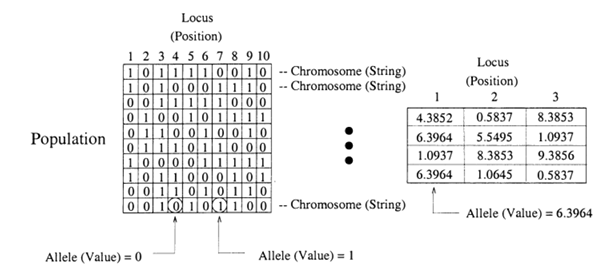
\includegraphics[width=\textwidth]{Figuras/EA_components.png}
    \caption[Componentes algoritmo evolutivo]{Descripción de componentes de la representación interna de un algoritmo evolutivo. En la parte izquierda tenemos una representación binaria, mientras que en la derecha una representación real de los individuos.}
    \label{fig:EA_components}
\end{figure}

Los algoritmos evolutivos cuentan con tres mecanismos para imitar la evolución natural que se representan en forma de diagrama en la Figura \ref{fig:EA_mech}, esta Figura fue traducida y adaptada de \cite{coelloEvolutionaryAlgorithmsSolving}. A continuación detallamos estos mecanismos: 

\begin{enumerate}
    \item Selección: Toma una función de aptitud $f$ que indica que tan bueno es cada individuo y se queda con los mejores con diferentes mecanismos como torneos. Al seleccionar los mejores individuos estamos reforzando algún camino escogido, invitando a que las futuras generaciones miren cerca de esa región del espacio de estados donde se encontró algo valioso. Este concepto, de buscar más donde ha habido mejores resultados es conocido como \textbf{Explotación}. En la Figura \ref{fig:explotacion} vemos 3 puntos en azul a los que se les permite dar 20 pasos de descenso de gradiente. Como vemos, de estos tres puntos se obtiene 
    un mínimo local. En este caso hubiera sido mejor buscar en el espacio de estados más, en vez de usar nuestras primeras opciones \\El mecanismo de selección tiene imita el proceso evolutivo biológico de la \emph{supervivencia del más apto}.
    \item Mutación: Se modifica de manera aleatoria el genotipo del individuo. Este procedimiento podría desviarnos de un individuo con una función de aptitud alta, sin embargo, la aleatoriedad hace que podamos buscar en más partes del espacio de búsqueda y no nos quedemos en un mínimo local. A esta estrategia de expandir el espacio de búsqueda se le conoce como \textbf{Exploración}. En la Figura \ref{fig:explotacion} vemos un análogo al de la Figura de \ref{fig:explotacion} sólo que en esta caso se ponen 10 puntos a explorar. De estos 10 puntos uno se encuentra cerca del último valle y puede obtener el máximo global. El balance de los dos es lo que un buen algoritmo evolutivo tendría idealmente. \\ El mecanismo de mutación es análogo a la mutación biológica, cuando se producen errores en la copia del código genético y estas modificaciones muestrean el espacio de posibilidades para un ser vivo.   
    \item Cruza: Se seleccionan dos individuos y se mezclan sus genes. Aquí también hay varios métodos, como cruza en $n$ puntos, etc. La cruza tiene un componente de explotación y de exploración ya que la combinación de dos genotipos no necesariamente dará como resultado a la misma combinación de sus fenotipos, podemos encontrar cosas inesperadas y en ese sentido tendría un aspecto de exploración. La parte que si mantiene de los individuos exitosos tendría un componente más de explotación. \\La cruza tiene un análogo natural en la reproducción de los seres vivos, la combinación de sus genes. 
\end{enumerate}

\begin{figure}[H]
    \centering
    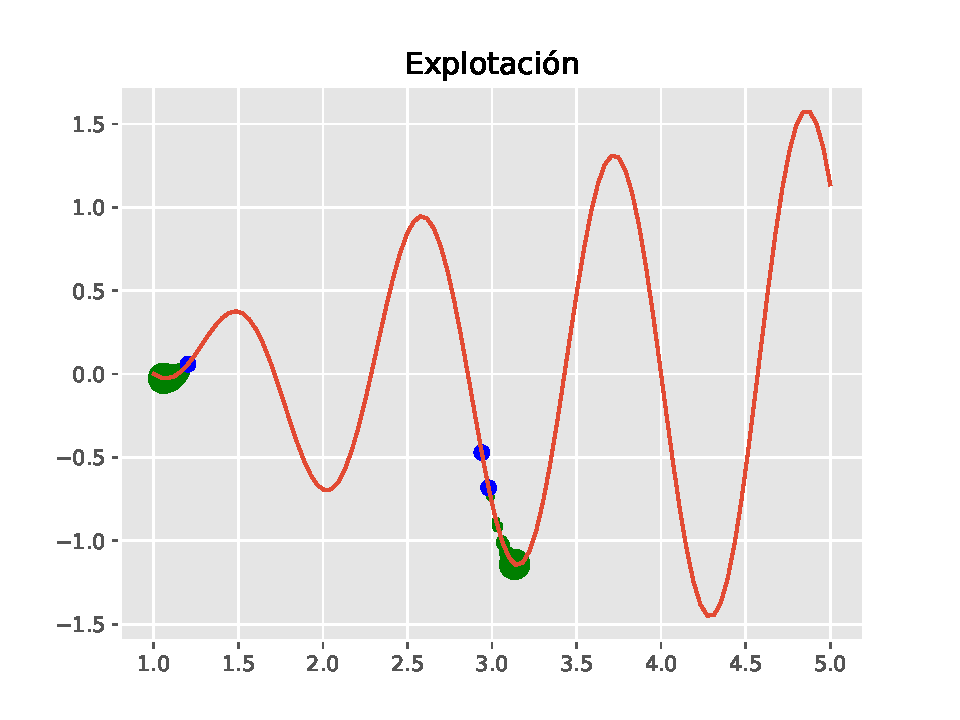
\includegraphics[width=\textwidth]{Figuras/explotacion.pdf}
    \caption[Explotación]{Estrategia de Explotación visualizada; dados los puntos haz más pasos de gradiente descendiente con ellos.}
    \label{fig:explotacion}
\end{figure}

\begin{figure}[H]
    \centering
    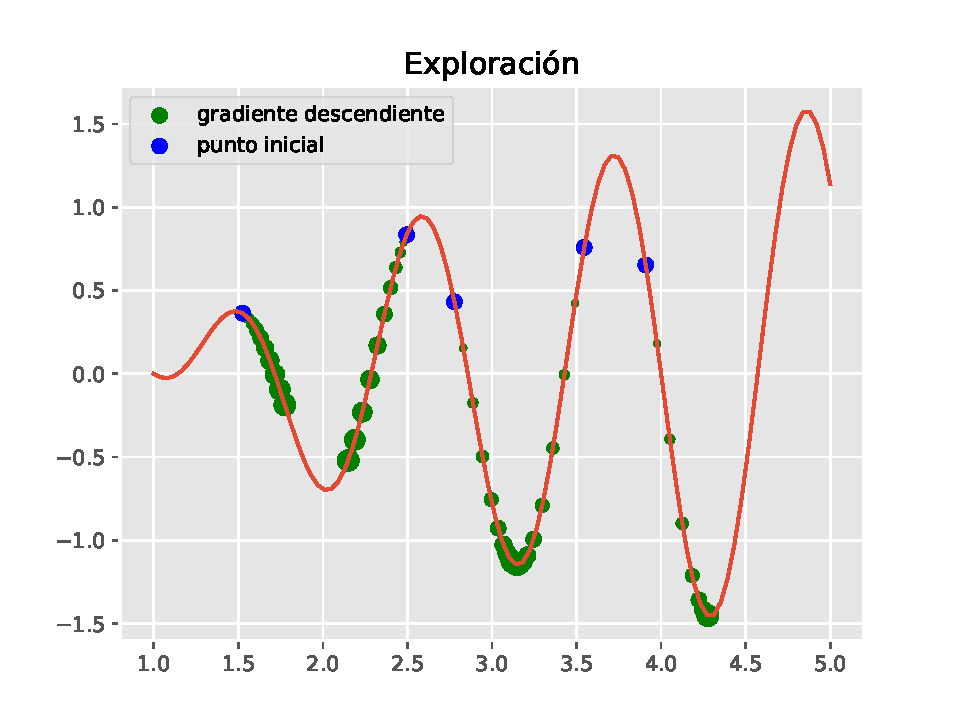
\includegraphics[width=\textwidth]{Figuras/exploracion.pdf}
    \caption[Exploración]{Estrategia de Exploración visualizada; dar menos pasos, pero desde más puntos.}
    \label{fig:exploracion}
\end{figure}

\begin{figure}[H]
    \centering
    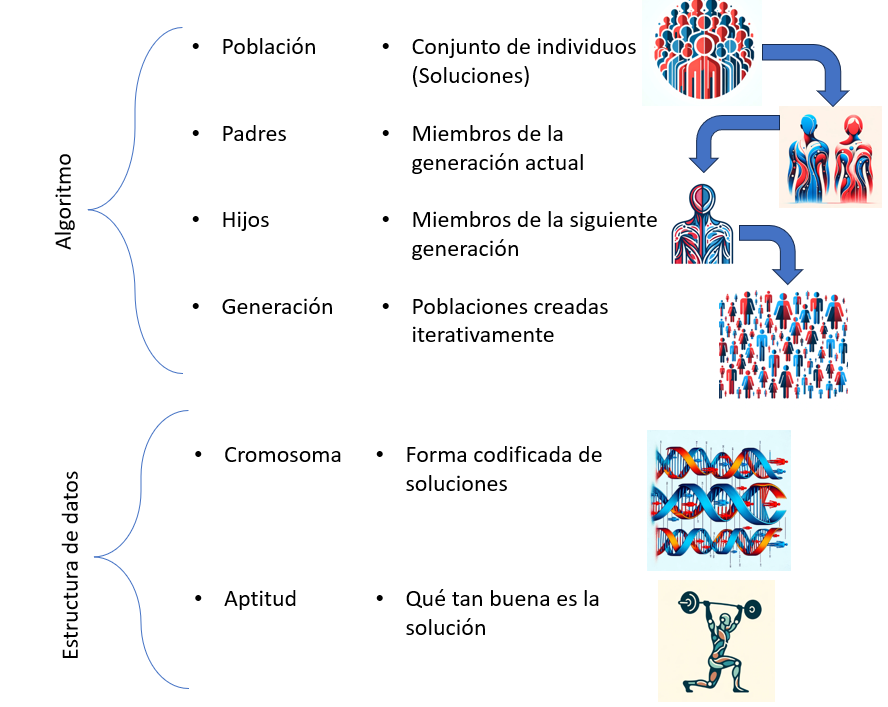
\includegraphics[width=\textwidth]{Figuras/AE_parts_algorithm.png}
    \caption{Ilustración del mecanismo básico del algoritmo evolutivo. }
    \label{fig:EA_mech}
\end{figure}

De manera formal definimos un algoritmo evolutivo de la siguiente forma \cite{coelloEvolutionaryAlgorithmsSolving}:


\begin{itemize}
    \item Sea $I$ un conjunto no vacío; el espacio de individuos. Un miembro de este conjunto, es decir, un inficiduo, vivirá en un espacio vectorial de dimensión igual a la del genotipo donde cada entrada corresponde a un gen dentro de un cromosoma. Así un individuo se denota como $\vec{a}$ y una población de $n$ individuos como como $\{\vec{a}_1,\ldots , \vec{a}_n\}$.
    \item Al ser un proceso iterativo indexamos las diferentes generaciones de individuos con el símbolo $i\in\mathbb{N}$.
    \item También denotamos como $I^\mu$ al conjunto de $\mu$ individuos. Así ${(I^{\mu})}^{(i)}$ corresponde a los $\mu$ individuos de la $i$-ésima generación. 
    \item $\{\mu^{(i)}\}, i\in \mathbb{N}$ una sucesión en $\mathbb{Z}^+$; el tamaño de las poblaciones de los padres. 
    \item $\phi: I\rightarrow R$; la función de aptitud.
    \item $\Psi: \bigcup_{i=1}^\infty (I^{\mu})^{(i)}\rightarrow \{0,1\}$; el criterio de término, 0 si no ha terminada y 1 si ya terminó. Es decir, la función $\Psi$ asigna a cada configuración de individuos una bandera de si el algoritmo debe continuar o no. Cuando se obtiene el desempeño deseado, la bandera cambiaría a verdadero (o el valor 1) y el algoritmo se detiene. 
    \item $m^{(i)}$; una sucesión de operadores de mutación, con sus respectivos parámetros. Este operador aumenta la \textbf{exploración} ya que nos permite muestrear otra parte del espacio de estados sin tomar en cuenta la aptitud de la función actual.
    \item $s^{(i)}$; una sucesión de operadores de selección, con sus respectivos parámetros. Este operador  se enfoca en la \textbf{explotación} porque toma en cuenta las soluciones que ya tienen buen desempeño en el espacio de estados para continuar el algoritmo. 
    \item $r^{(i)}$; una sucesión de operadores de recombinación, con sus respectivos parámetros. Es decir, el operador que toma dos poblaciones y mezcla los individuos para producir una nueva población.  En este caso se tiene una combinación de exploración y explotación. Por un lado, se explora porque se produce un individuo nuevo con cierto grado de aleatoriedad (dependiendo del mecanismo explícito de recombinación esto puede ser mayor o menor). Por otro lado, fomenta la explotación al combinar elementos que ya pasaron una prueba se delección. 
    \item $\chi$ un booleano que indica si el algoritmo tomará sólo la población actual o también la anterior para seleccionar los más aptos.
\end{itemize}

Entonces el pseudocódigo del algoritmo evolutivo general está dado por

\begin{algorithm}
    \caption{Algoritmo Evolutivo}\label{alg:EA}
    \begin{algorithmic}[1] % The number indicates line numbering step
    \State t:=0;
    \State Inicializa $P(0):=\{a_1(0),\ldots,a_\mu(0)\} \in I^{\mu^{(0)}}$;
    \While{$\Psi(\{P(0),\ldots,P(t)\}) \neq 1 $} \do ; 
        \State $\textit{recombina}: P'(t)=r^{(t)}(P(t))$;
        \State $\textit{muta}: P''(t)=m^{(t)}(P'(t))$;
        \State $\textit{selecciona}$:
            \If{$\chi$}
                \State $P(t +1):= s^{(t)}(P''(t))$;
                \Else  $P(t +1):= s^{(t)}(P''(t) \cup P(t))$
            \EndIf
    $t=t+1$;    
    \EndWhile
    \textbf{EndWhile}
\end{algorithmic}
\end{algorithm}

El Algoritmo \ref{alg:EA} sigue los pasos descritos a continuación: El proceso inicia con la inicialización del contador de generaciones en $t=0$. Seguidamente, se establece la primera población de individuos, donde cada uno se identifica con un subíndice que denota su posición en una población de tamaño $\mu$ y se anota entre paréntesis el número de la generación correspondiente, que para esta fase inicial es la generación 0. En la tercera línea del algoritmo, se establece que, mientras la condición de paro $\Psi$ devuelva 0, el proceso de generación de nuevos individuos continúa. Las líneas 4 y 5 están dedicadas a aplicar los operadores de recombinación y mutación, respectivamente. Del paso 6 al 9, se ejecuta el operador de selección, donde la función de aptitud $\phi$ está implícita como parte de este proceso. Este proceso depende de la bandera $\chi$: si $\chi$ es verdadera, la selección se realiza únicamente a partir de la nueva población; en cambio, si $\chi$ no es verdadera, la selección incluye tanto a los nuevos individuos como a aquellos de la generación anterior. Finalmente, se incrementa el contador de selección y el algoritmo se mantiene en este estado operativo hasta que la condición de paro deja de cumplirse y se sale del bucle \textit{While}.

Una distinción importante que hay que realizar para algoritmos evolutivos es cuando en cada paso de selección de población, se retienen los mejores individuos de la generación actual o si se sustituyen completamente con sus descendientes. Al primer tipo de algoritmos se les conoce como \textbf{elitistas} y los otros son conocidos como \textbf{no-elitistas}. Se les suele distinguir por la siguiente notación $(\mu+\lambda)$ significa que los hijos competirán por $\mu$ lugares (es decir es elitista) mientras que la notación $(\mu,\lambda)$ significa que se sustituirán los $\mu$ padres con $\lambda$ hijos. La idea detrás de los algoritmos elitistas es no perder información valiosa que se haya obtenido a lo largo del proceso de búsqueda, en este sentido podría ser considerado como una parte más de explotación sin llegar a enfocarse mucho en una parte del espacio de búsqueda. Sólo manteniendo la referencia de que en esa parte del espacio había una avenida que vale la pena explorar con operadores de mutación y cruza que fomentan la exploración.
    
Los algoritmos evolutivos se han usado para resolver problemas multiobjetivo por su enfoque en poblaciones y aproximaciones en casos donde no se puede encontrar una solución analítica. El primer algoritmo evolutivo multiobjetivo (MOEA por sus siglas en inglés) fue dado por David Schaeffer en 1984 en su tesis doctoral \cite{schafferMultipleObjectiveOptimization1984}, su propuesta llamada VEGA (Vector Evaluation Genetic Algorithm) y pretendía resolver problemas de aprendizaje de máquina.

En el Ejemplo \ref{ex:Selecc} que se ha estado revisando de hacer una selección de características de un problema de clasificación  ha sido abordado usando algoritmos evolutivos desde 1985 \cite{SIEDLECKI1989335} aunque en este caso se pretendía como un problema SOP con una restricción en el número de columnas. 


Para definir un MOEA basta cambiar la definición de la función de selección $\phi$ en el algoritmo evolutivo usual presentada en el Algoritmo \ref{alg:EA}. Esta función es la de aptitud, que ahora en el caso multiobjetivo, tendrá que ser evaluada en muchos objetivos. Así tenemos que pasamos de $\phi:I\rightarrow \mathbb{R}$ a

$$\phi:I\rightarrow \mathbb{R}^{n_{obj}}, \quad n_{obj}>1.$$


Podemos ver una descripción pictórica en la Figura \ref{fig:MOEA_EA}.

\begin{figure}[H]
    \centering
    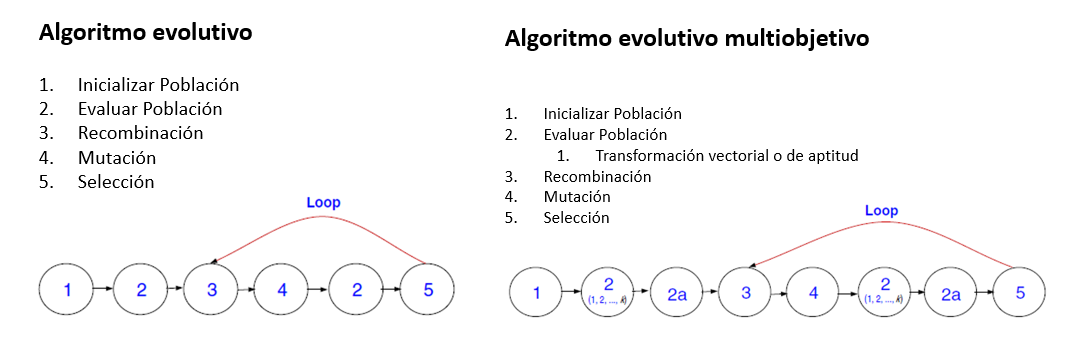
\includegraphics[width=\textwidth]{Figuras/MOEA_EA.png}
    \caption[MOEAs vs EAs]{Diferencia entre los procedimientos para uno a) y múltiples objetivos b). La diferencia es la transformación y evaluación vectorial. Imagen traducida de \cite{coelloEvolutionaryAlgorithmsSolving}.}
    \label{fig:MOEA_EA}
\end{figure}


En el contexto de algoritmos evolutivos para problemas multiobjetivo se le suele llamar \textbf{conjunto de aproximación} a la población que se obtiene paso a paso. Denotamos $\Psi$ al conjunto de todas las aproximaciones; es decir, al conjunto de todos los conjuntos finitos del espacio objetivo. Además se le llama \textbf{aproximación al frente de Pareto} a aquel $\psi$ en el conjunto de aproximación $\Psi$ tal que no existe ninguna solución en $\psi$ que domine a otra. 




           % ~20 páginas - Poner un contexto a la tesis, hacer referencia a trabajos actuales en el tema

%%%%%%%%%%%%%%%%%%%%%%%%%%%%%%%%%%%%%%%%%%%%%%%%%%%%%%%%%%%%%%%%%%%%%%%%%
%           Capítulo 3: NOMBRE                   %
%%%%%%%%%%%%%%%%%%%%%%%%%%%%%%%%%%%%%%%%%%%%%%%%%%%%%%%%%%%%%%%%%%%%%%%%%

\chapter{Algoritmos Evolutivos para problemas Multiobjetivo}

Resolver un MOP requeriría obtener todo el conjunto y el frente de Pareto. Sin embargo, esta tarea es muy complicada. Además, debido a que los objetivos frecuentemente se comportan como cajas negras y el espacio de búsqueda es muy grande, obtener el frente de Pareto exacto con algún método algorítmico es frecuentemente una tarea imposible \cite{SMS-EMOA}. 

Una manera de abordar este problema, que es la que usaremos en este trabajo, es encontrar una representación del frente usando individuos de una población que se va iterando para aproximar puntos que cada vez representen más fielmente al frente de Pareto.

El capítulo se organizará de la siguiente forma: en la Sección \ref{sec:QIs} se revisan los indicadores de calidad usados en este trabajo, después, en la Sección \ref{sec:QIs_tax} se explica cómo se clasifican los EMOAs de acuerdo a sus diferentes estrategias, ya sea dentro del algoritmo evolutivo mismo (si son elitistas o no), así como en su mecanismo de selección, etc. Revisaremos con especial cuidado en la Sección \ref{sec:Metodos_QI} aquellos algoritmos que calculan de cada población diversos indicadores de calidad para tener una mejor representación del frente de Pareto (IB-EMOA por sus siglas en inglés), revisando cada uno de los indicadores que usaremos en este trabajo. 

Después, en la Sección \ref{sec:SMS-EMOA} estudiaremos un algoritmos antecedente al usado en este trabajo. El antecedente es el algoritmo prototípico IB-EMOA, llamado SMS-EMOA. Continuaremos con el algoritmo usado en este trabajo en la Sección \ref{sec:PFI-EMOA}. Dicho algoritmo recibe el nombre de PFI-EMOA y fue diseñado para combinar dos indicadores de calidad dentro de su proceso de selección. Finalmente, concluiremos en la Sección \ref{sec:pruebas_estadisticas} con una breve descripción de cómo se comparan diferentes algoritmos entre sí usando pruebas estadísticas.

\section{Indicadores de calidad} \label{sec:QIs}
Al ser un MOP, por definición, un problema que requiere hacer concesiones en cada objetivo, necesariamente habrá varias maneras de comparar dos conjuntos de aproximación para decidir qué conjunto es mejor. La primera de ellas concierne a la dominancia de Pareto entre conjuntos de aproximaciones, siendo esta una extensión del concepto de dominancia entre puntos, como vimos en la Sección \ref{sec:Dominancia_Pareto}. Al extender el concepto a dominancia entre conjuntos, ya no se hace una sólo comparación. Por lo tanto, existen más posibilidades que cubrir, y por ende, más elecciones que tomar. Considerando a dos conjuntos de soluciones $A,B \subseteq \mathbb{R}^m$ en el espacio de objetivos,  veremos algunas manerad de compararlos, definidas en \cite{tesis_mst_guillermo}.

% Se dice que $x$ \textbf{domina débilmente} a $y$, denotado como $x \preccurlyeq y$  si $f_i(x)\leq f_i(y)$ para toda $i\in\{1,\ldots,m\}$; es decir $x$ no es peor (mayor si queremos maximizar o menor si queremos minimizar) que $y$ en ningún objetivo \footnote{Algunas definiciones también piden que $x\neq y$}.  Si además existe un objetivo tal que es peor en alguna dirección, es decir $\exists i \in\{1,\ldots,m\}$ tal que $f_i(x)< f_i(y)$  entonces $x$ \textbf{domina} a $y$, denotado como $x \prec y$. Aún podemos pedir que la relación sea más clara si pedimos $f_i(x)< f_i(y)$, $\forall i \in\{1,\ldots,m\}$. A esta relación se le conoce como \textbf{dominancia estricta}. Esta propiedad dice que una solución es mejor a la otra en todos sus objetivos y se denota como $x \prec \prec y$.


% Una solución $x$ se le llama \textbf{óptima de Pareto} o \textbf{eficiente de Pareto} si no existe ninguna otra solución $y$ tal que $y \prec x$. Es decir si es parte de las mejores soluciones que podemos encontrar. Al conjunto de soluciones eficientes de Pareto se le conoce como \textbf{frente de Pareto}.

% Al intentar definir una única noción de que un conjunto de soluciones sea mejor que otro encontranos, al igual que en la noción de dominancia, que es útil crear definiciones cada vez más estrictas. A continuación se listan algunas de ellas: 

\begin{itemize}
    \item \textbf{Definición 1 (Dominancia Débil)}: Un conjunto \( A \) se dice que domina débilmente a \( B \) si cada solución \( b \in B \) está débilmente dominada por al menos una solución \( a \in A \) y $A\neq B$. Se denota $ A \preceq B$.  Esta es la forma más general y menos restrictiva de las jerarquías entre conjuntos.
    \item \textbf{Definición 2 (Mejor)}: U Se denota a con $ A \vartriangleleft   B$, también conocida como sobredesempeño débil ($A \ \ \mathcal{O}_W \ B$). Es equivalente a decir que $A \preceq B$, pero $B \npreceq A$. En palabras es que $A$ es al menos tan bueno como $B$, mientras que $B$ no es tan bueno como $A$. 
    
    \item \textbf{Definición 3 (Sobredesempeño Fuerte)}: Un conjunto \( A \) se dice que rinde fuertemente a \( B \) si \( A \) domina débilmente a \( B \) y además existe al menos un par de soluciones \( a \in A \) y \( b \in B \) tal que \( a \) domina a \( b \). Denotado $A \ \ \mathcal{O}_S \ B$.
    \item \textbf{Definición 4 (Dominancia)}: Un conjunto \( A \) se dice que domina a \( B \) si cada solución \( b \in B \) está dominada por al menos una solución \( a \in A \). Se denota $A \prec B$. Es importante recalcar que esta medida de dominancia define un orden parcial en el espacio de aproximaciones.
    \item \textbf{Definición 5 (Dominancia Estricta)}: Un conjunto \( A \) se dice que domina estrictamente a \( B \) si cada solución \( b \in B \) está estrictamente dominada por al menos una solución \( a \in A \). Se denota $ A \prec \prec B$, también es llamado sobredesempeño completo $A \ \ \mathcal{O}_C \ B$.
\end{itemize}



Es útil ver las contenciones de las definiciones previas ya que una solución será preferida en este sentido mientras más nos desplazamos hacia el conjunto más pequeño. Así, tenemos 

\begin{align} \label{eq:contencion_comp_sets}
    A \prec \prec B \implies A \prec B &\implies A \ \mathcal{O}_S \ B  \nonumber\\
    \implies A \vartriangleleft B &\implies A\preceq B. \nonumber
\end{align}


En un problema, sin embargo, las nociones de dominancia previamente definidas no se tienen que alinear con todas las preferencias de un tomador de decisiones. Es decir, es posible que un conjunto $A$ que sea, por ejemplo, \textbf{mejor} (en el sentido de la Definición 2) que otro $B$ y que, sin embargo, haya soluciones en $B$ que dominen a algunas de $A$. Para lidiar con estos problemas sería preferible encontrar un conjunto de soluciones que sea una buena representación del frente de Pareto. Así, al preguntarnos qué características son deseables en un algoritmo que busque una representación fidedigna al frente de Pareto encontramos la razón de la construcción de los  \textbf{indicadores de calidad} (QI por sus siglas en inglés).


Con el fin de estudiar propiedades generales de los frentes, se han propuesto categorías de características deseables en la representación del frente:

\begin{itemize}
    \item \textbf{Proximidad o convergencia}: La proximidad que tiene con el frente de Pareto. El tipo de relación que medimos con las definiciones 1 a 5. 
    \item \textbf{Extensión}:  El tamaño de la región que ocupa el conjunto de soluciones. 
    \item \textbf{Uniformidad}: Que tan equidistantes son las soluciones entre sí.
    \item \textbf{Diversidad}: Como extensión y uniformidad suelen intersectar sus objetivos se les suele combinar en la categoría de diversidad, como, por ejemplo, en el estimador de densidad de NSGA-II, explicado en la Sección \ref{sec:nsga2}. 
\end{itemize}

Estos conceptos se  entienden mejor al estudiar la Figura \ref{fig:carac_deseables_aprox}. De las características previamente mencionadas tenemos las siguientes: 

\begin{itemize}
    \item I. tiene buena convergencia y extensión, pero mala uniformidad.
    \item II. tiene bien todo excepto convergencia.
    \item III. tiene muy poca extensión.
    \item IV. tiene todas las características deseables.
\end{itemize}

Incluso intuitivamente, podemos ver que en cada uno de los casos que no son el IV hay deficiencias en las aproximaciones al frente de Pareto. 

\begin{figure}[H]
    \centering
    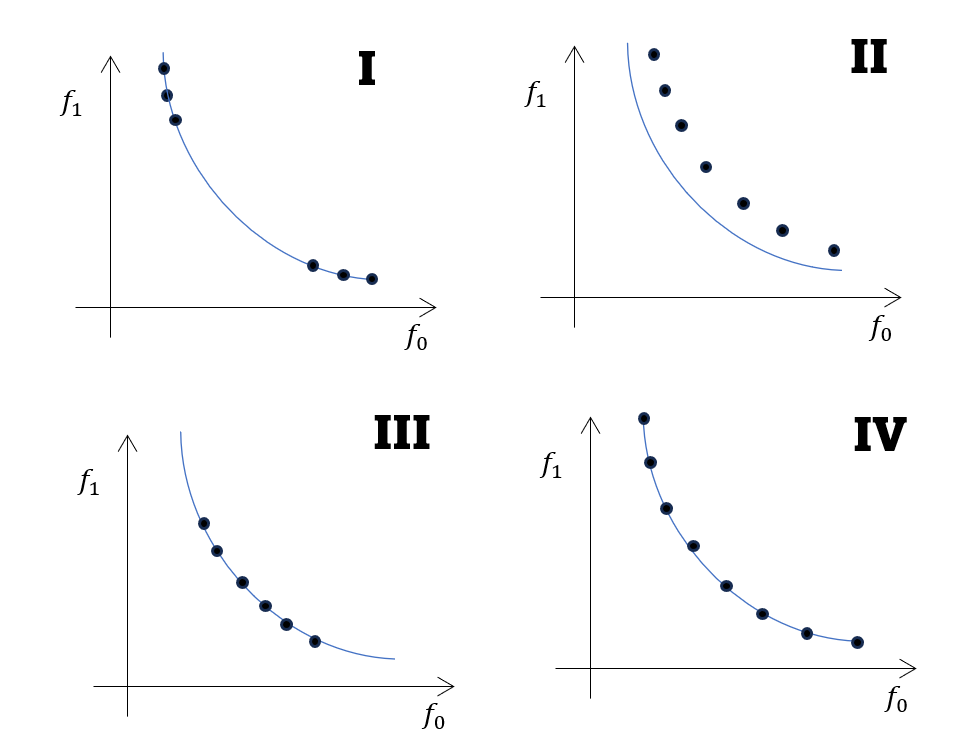
\includegraphics[scale=0.5]{Figuras/carac_deseables_Pareto.png}
    \caption[Características deseables en aproximación al PF]{Características deseables en aproximaciones al frente de Pareto (puntos) y el frente de Pareto como una línea.}
    \label{fig:carac_deseables_aprox}
\end{figure}

Estos indicadores también se pueden clasificar de acuerdo al número de conjuntos de soluciones con los que operan. Si el indicador opera sobre un único conjunto  se le llama un operador unario, mientras que si compara $n$ conjuntos se le llama $n$-ario. Formalmente un indicador $n$-ario \cite{PFI} es  una función que manda  $n$ conjuntos de soluciones a un número real. Es decir $I:\psi_1,\cdots,\psi_n \rightarrow \mathbb{R}$ con $\psi_i \in  \Psi$, el conjunto de aproximaciones, para todo $i$. 


Al ser un mapeo a los números reales, es posible definir un orden total en $\Psi$ a través de un indicador unario. Dicho orden puede coincidir con aquel de la dominancia de Pareto en el siguiente sentido

\begin{equation} \label{eq:consistente_Pareto}
    A \vartriangleleft B \implies I(A) < I(B).
\end{equation}
A esta propiedad del indicador $I$ se le conoce como \textbf{consistencia de Pareto}. Cuando la condición es de desigualdad, es decir 

\begin{equation} \label{eq:consistente_debil_Pareto}
    A \vartriangleleft B \implies I(A)\leq I(B),
\end{equation}

se le llama consistencia débil.

No siempre es posible que nuestro indicador sea consistente de Pareto, por ejemplo, en categorías como diversidad no necesariamente se alinearan los objetivos de esparcir un conjunto con aquellos de encontrar uno menos dominado. Esto se debe a que el esfuerzo de definir indicadores que no sólo traten de dominancia es para no caer en las situaciones donde tratar el problema de esta forma lleva a complicaciones como que el algoritmo se estanque.

A continuación definiremos brevemente los indicadores usados en este trabajo .

\subsection{Hipervolumen} \label{sec:HV}

Se presentó por primer vez en \cite{zitzlerMultiobjectiveOptimizationUsing1998} como una medida del espacio cubierto y se suele abreviar como HV. 
El hipervolumen se construye con un punto de referencia y indica cuál es el tamaño del espacio dominado entre nuestro conjunto y el punto de referencia. Es un operador unario por lo que es muy conveniente usarlo aún cuando no se conoce el frente de Pareto. La sensibilidad de este indicador recae en la elección del punto de referencia; dicho  punto debe ser escogido de manera que sea dominado por todos los puntos del frente. Se puede escoger, por ejemplo, el punto de Nadir, vista en la Definición \ref{def:Nadir}, ya sea sólo o multiplicado por 1.1 para tenerlo un poco alejado. Sin embargo, no hay un consenso de cómo escoger el punto y diferentes puntos de referencia pueden llevar a una evaluación inconsistente \cite{HV_ref_point}. De modo que es importante, al comparar algoritmos, que se establezca una convención del punto de referencia. El hipervolumen es muy usado porque es consistente de Pareto \eqref{eq:consistente_Pareto} y está definido por la siguiente ecuación 

\begin{equation} \label{eq:HV}
    \text{HV}(A)=\lambda\left( \bigcup_{a\in A} \{x|a \prec x \prec r \} \right), \nonumber
\end{equation}
donde $\lambda$ es la medida de Lebesgue y mide el hipervolumen de la unión de los hipercubos definidos por cada una de las soluciones $a$ que viven en $A$ y el punto de referencia $r$. Así para cada uno de los conjuntos, los puntos $x$ serían aquellos que están entre el punto de la solución $a$ y el pinto de referencia $r$. Como podemos ver en la Figura \ref{fig:HV}.

\begin{figure}[H]
    \centering
    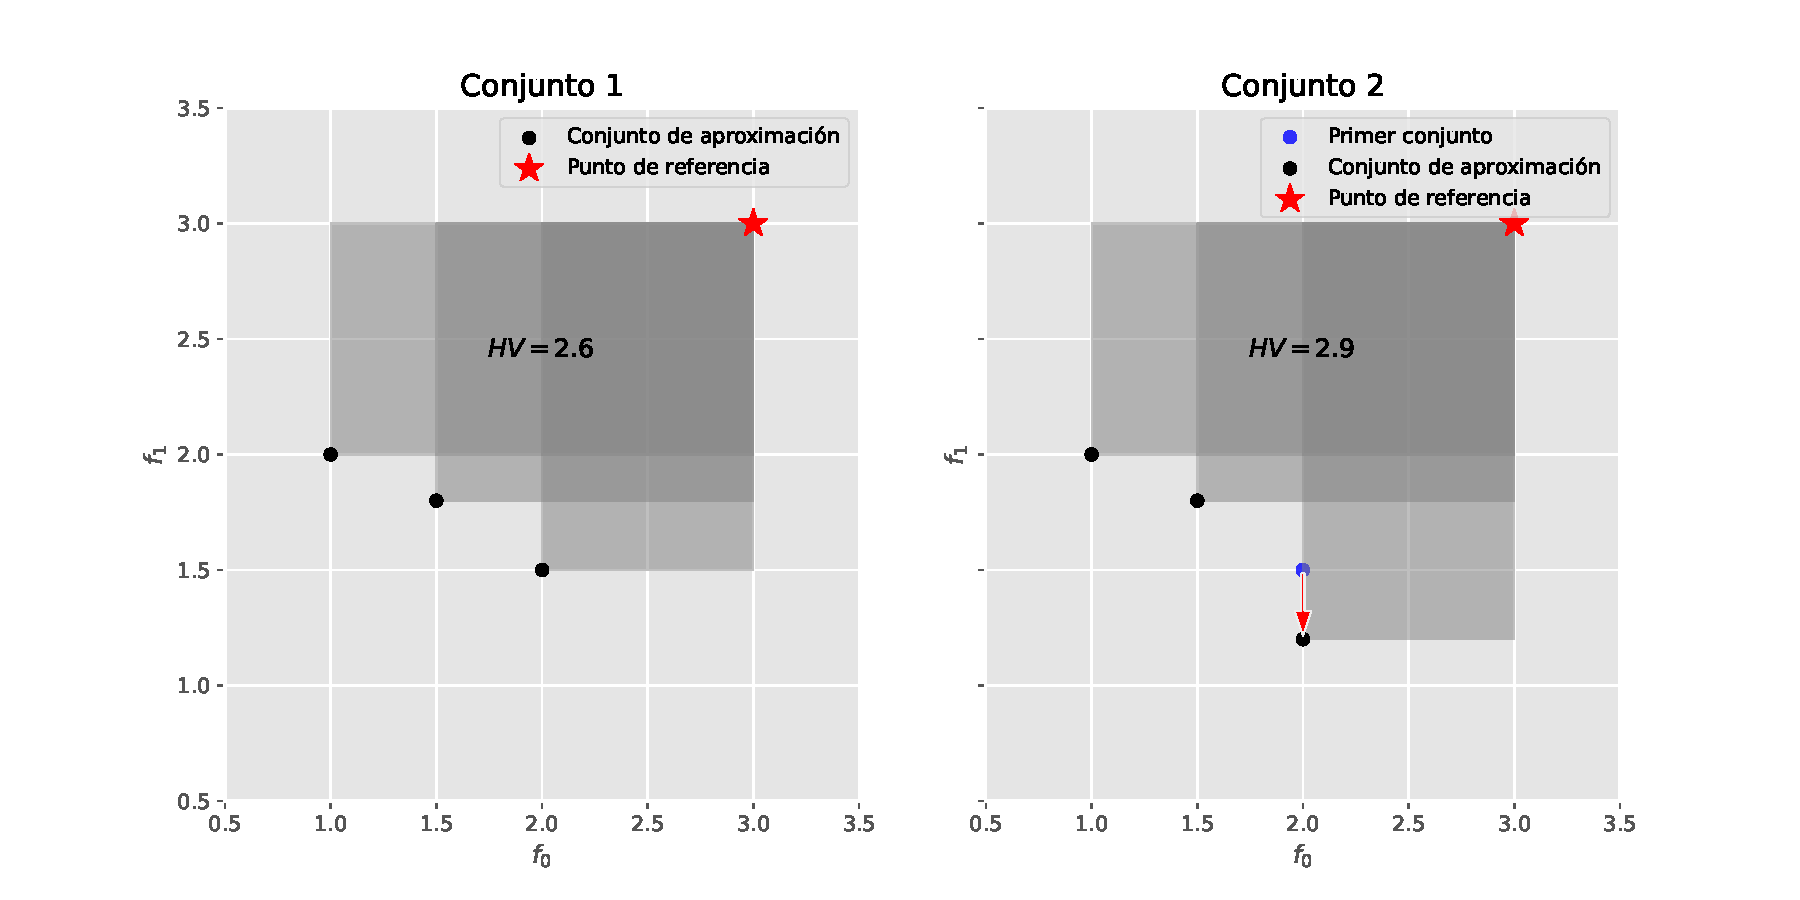
\includegraphics[scale=.6]{./Figuras/HV_demo.pdf} 
    \caption[Hipervolumen]{Cálculo del indicador HV para dos conjuntos, podemos ver su espacio dominado. Del lado derecho movemos sólo un punto hacia un menor $f_1$ y vemos que el HV toma en cuenta este aumento.}
    \label{fig:HV}
\end{figure}

Otra característica deseable de este indicador es que se probó en \cite{Measure_Pareto_Optima} que para un espacio de búsqueda finito y un punto de referencia, la maximización del hipervolumen equivale a encontrar el conjunto de Pareto. 

\subsection{Distancia Generacional (GD)} \label{sec:GD}
Este es un indicador binario en el que asumimos que tenemos un conjunto de referencia, idealmente este conjunto es la mejor representación del frente de Pareto posible. Fue introducido en \cite{GD}.

La idea del indicador es simplemente medir la distancia entre un conjunto de aproximación $\mathcal{A}$, que produciríamos con un algoritmo, al conjunto de referencia $\mathcal{Z}$. Así obtenemos la siguiente ecuación.

\begin{equation} \label{eq:GD}
    \text{GD} \left( \mathcal{A},\mathcal{Z} \right) = \frac{1}{|\mathcal{A}|} \sum_{x\in A} d_{\min}(x,Z)
\end{equation}

donde $d_{\min}(x,Z)=\min_{z \in \mathcal{Z}}{d(x,z)}$, con $d(x,y)$ una función de distancia, por ejemplo la norma euclidiana usual. En la Figura \ref{fig:GD_demo} podemos observar los conjuntos de aproximación $A$ y $B$ y los puntos mínimos con los que se calcula $d_{\min}$. Vemos que el conjunto $B$ al ser cercano a un punto del conjunto de referencia tiene un menor $\text{GD}$ que $A$.

\begin{figure}[H]
    \centering
    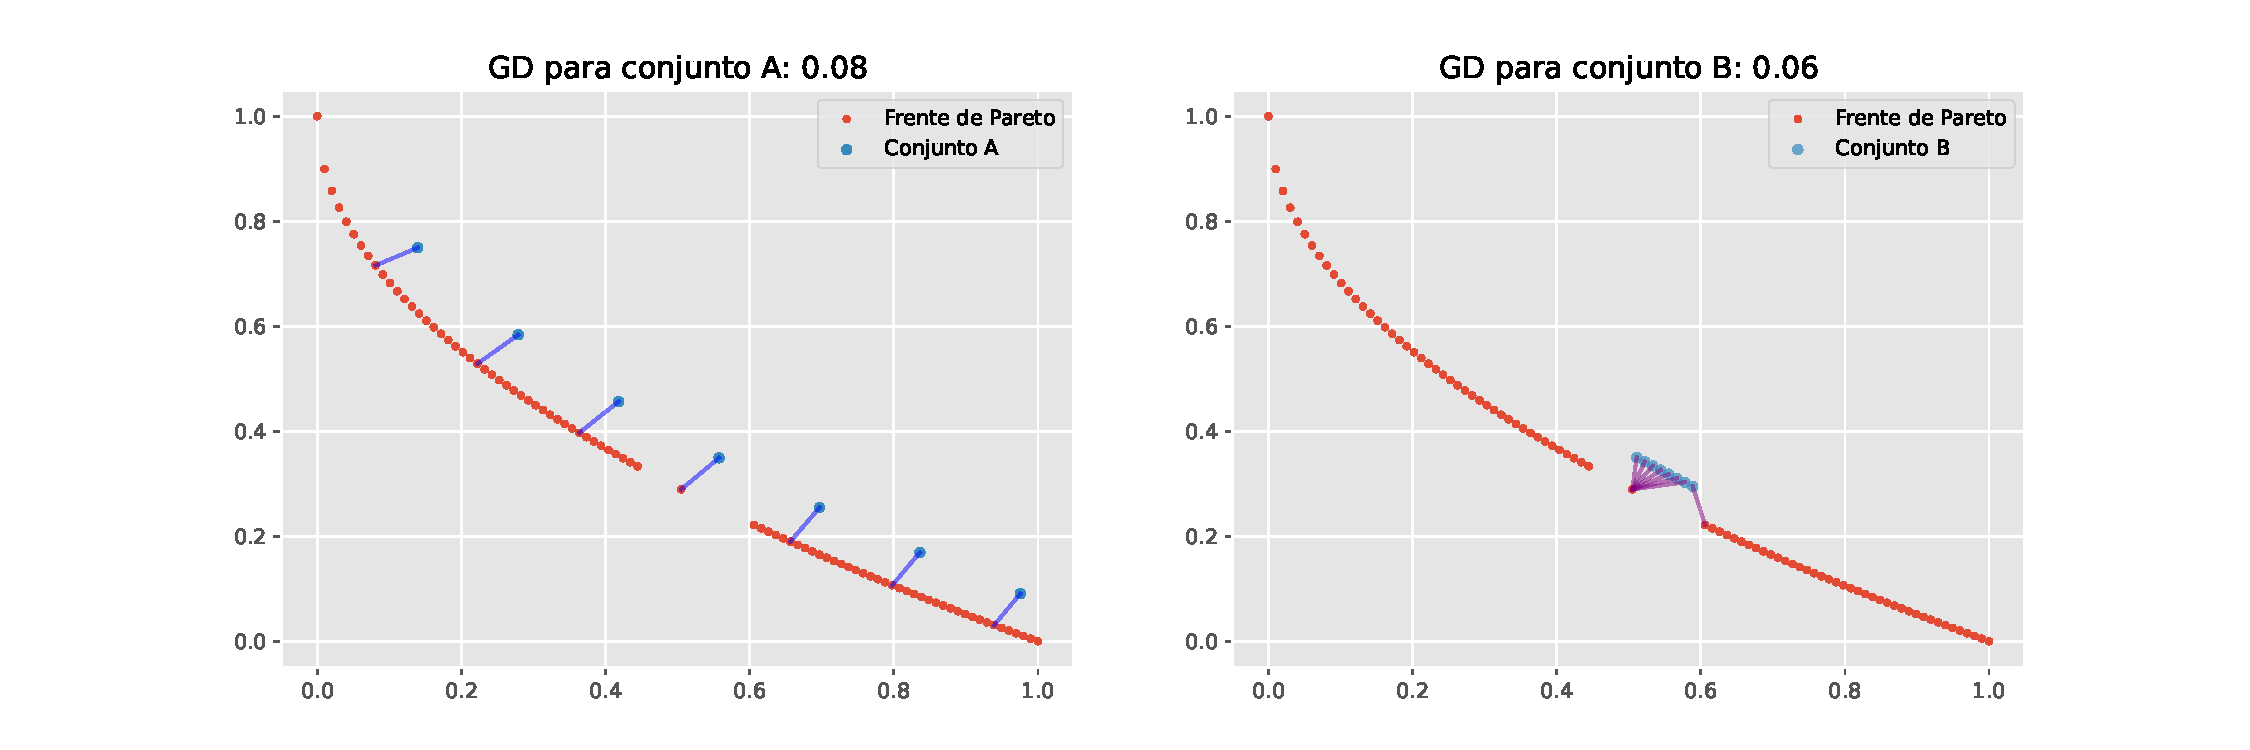
\includegraphics[width=\textwidth]{Figuras/GD_demo.pdf}
    \caption[GD]{Ilustración del cálculo del indicador GD para dos conjuntos.}
    \label{fig:GD_demo}
\end{figure}

\subsection{Distancia Generacional Invertida (IGD)} \label{sec:IGD}
Propuesta por primera vez en \cite{IGD}, la distancia generacional (IGD) invertida mide la distancia del $\mathcal{Z}$ de referencia al conjunto de aproximación, es decir sólo intercambiamos $\mathcal{A}$ y $\mathcal{Z}$ con respecto a la Ecuación \ref{eq:GD}.

\begin{equation} \label{eq:IGD}
    \text{IGD}(A,\mathcal{Z})=\frac{1}{|\mathcal{Z}|}\sum_{z\in\mathcal{Z}} d_{\min}(z,\mathcal{A}), \nonumber
\end{equation}
donde $d_{\min}(x,Z)=\min_{z \in \mathcal{Z}}{d(x,z)}$, con $d(x,y)$ una función de distancia. Esta definición permite tratar casos que GD favorecería y que usalmente no cumplen con requisitos como la diversidad. En la Figura \ref{fig:IGD_demo} vemos la diferencia de calcular ambos indicadores para los mismos conjuntos que en \ref{fig:GD_demo}. En particular, notamos cómo IGD si distingue entre ambos conjuntos, teniendo un valor más pequeño para el conjunto que tiene mejor diversidad.

\begin{figure}[H]
    \centering
    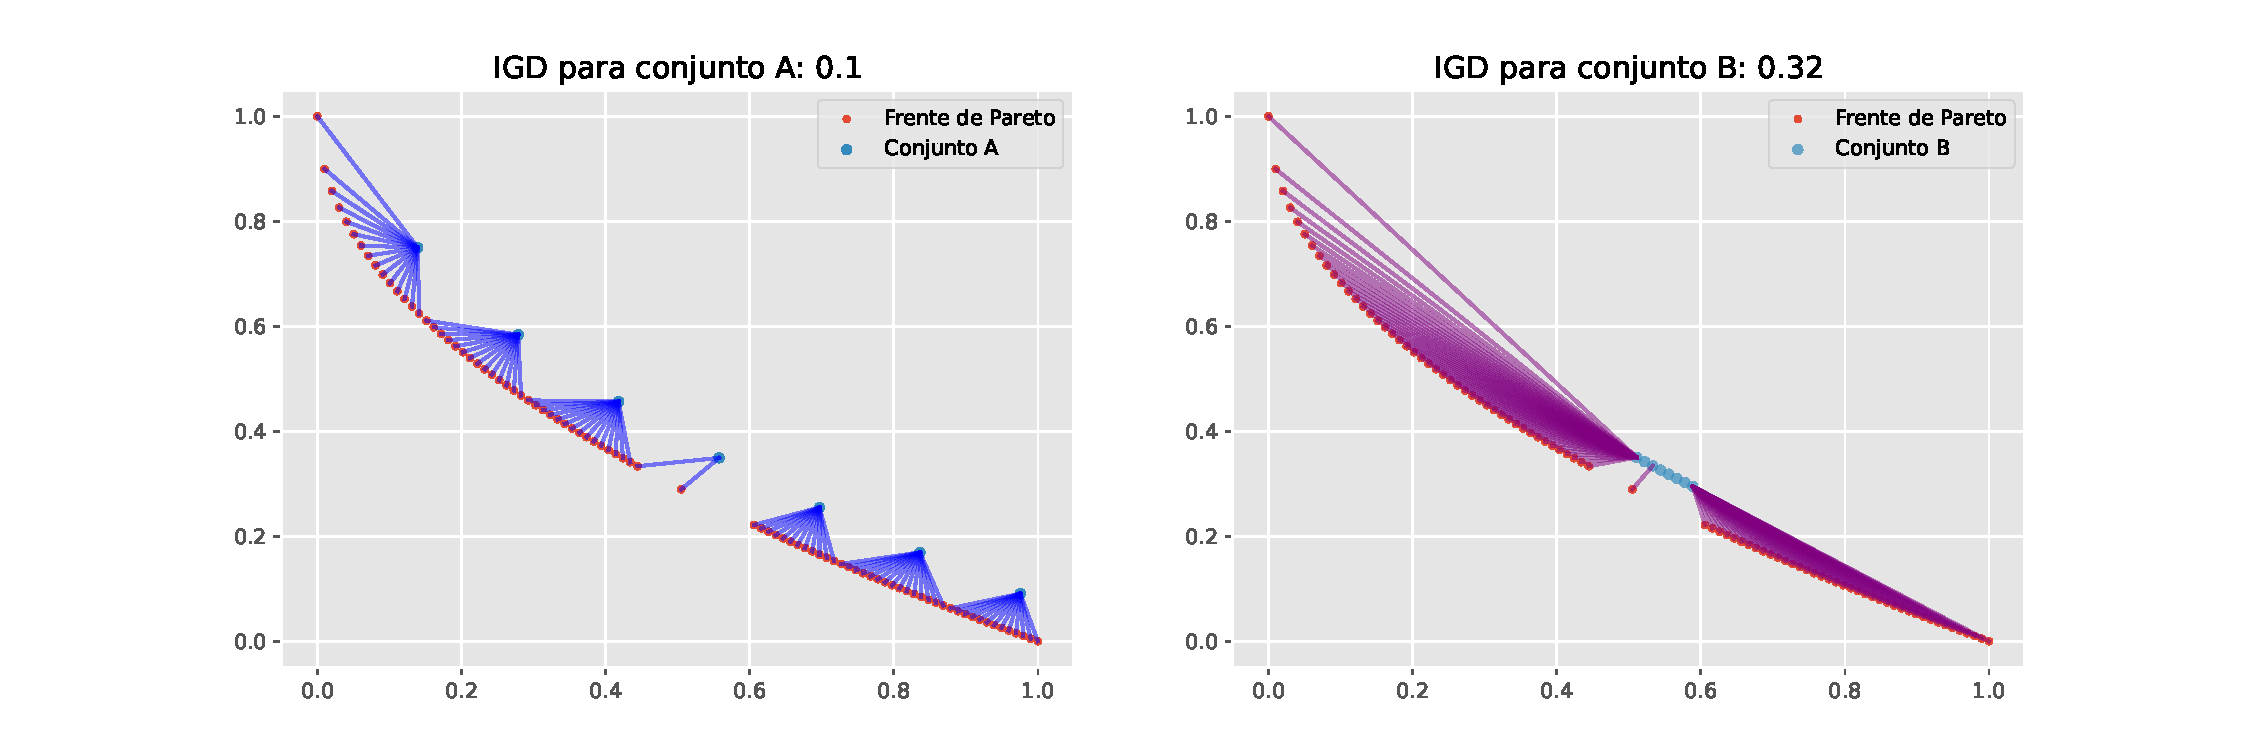
\includegraphics[width=\textwidth]{Figuras/IGD_demo.pdf}
    \caption[IGD]{Ilustración del cálculo del indicador IGD para dos conjuntos.}
    \label{fig:IGD_demo}
\end{figure}


\subsection{Distancia Generacional Invertida + (IGD +)} \label{sec:IGDp}
Definido en \cite{ishibuchiModifiedDistanceCalculation2015}, y denotado como IGD+, es una variación del indicador IGD en donde se usa una función de distancia euclidiana modificada dentro del cálculo del promedio. Si denotamos como $Z$ al conjunto de soluciones, $A$ al conjunto de al frente de Pareto, La ecuación tiene una forma similar a la de IGD usual, la diferencia es que usa la siguiente definición de distancia entre el conjunto de referencia y el de aproximación, dada por $$d^{+}(\vec{a},\vec{z})=\sqrt{\sum_{i=1}^m \max(a_i-z_i,0)^2} $$

Entonces la ecuación para el indicador queda como

\begin{equation} \label{eq:IGDp}
    \text{IGD}^+(A,Z) =  \frac{1}{|Z|} \sum_{\vec{z}\in Z}\min_{\vec{a}\in A} d^{+}(\vec{a},\vec{z}).
\end{equation}


Esta modificación hace al indicador uno débilmente consitente de Pareto (definido en la Ecuación \ref{eq:consistente_debil_Pareto}) que como hemos mencionado es una propiedad deseable de un indicador de convergencia. Regresando a la Ecuación \ref{eq:IGDp}, como $\vec{a}$ pertenece al conjunto de referencia y $\vec{z}$ al de aproximación, la Ecuación \ref{eq:IGDp} indica que, por cada dimensión, si la aproximación $z_i$ domina a la solución $a_i$ se calcula la distancia euclidiana usual. En caso contrario se calcula la distancia entre la aproximación $z$ y la región dominada de la referencia $a$. Al ser una medida de distancia, es mejor mientras sea más pequeña. En la Figura \ref{fig:comp_IGD_IGDp} podemos ver dos conjuntos distintos  en el que el conjunto $B$ incluso domina al conjunto de referencia, sin embargo, IGD nos diría que el conjunto $A$ es mejor al tener un menor valor del indicador. Con la modificación dada por la Ecuación \ref{eq:IGDp}, el indicador puede identificar que el conjunto $B$ domina al conjunto $A$.

\begin{figure}[H]
    \centering
    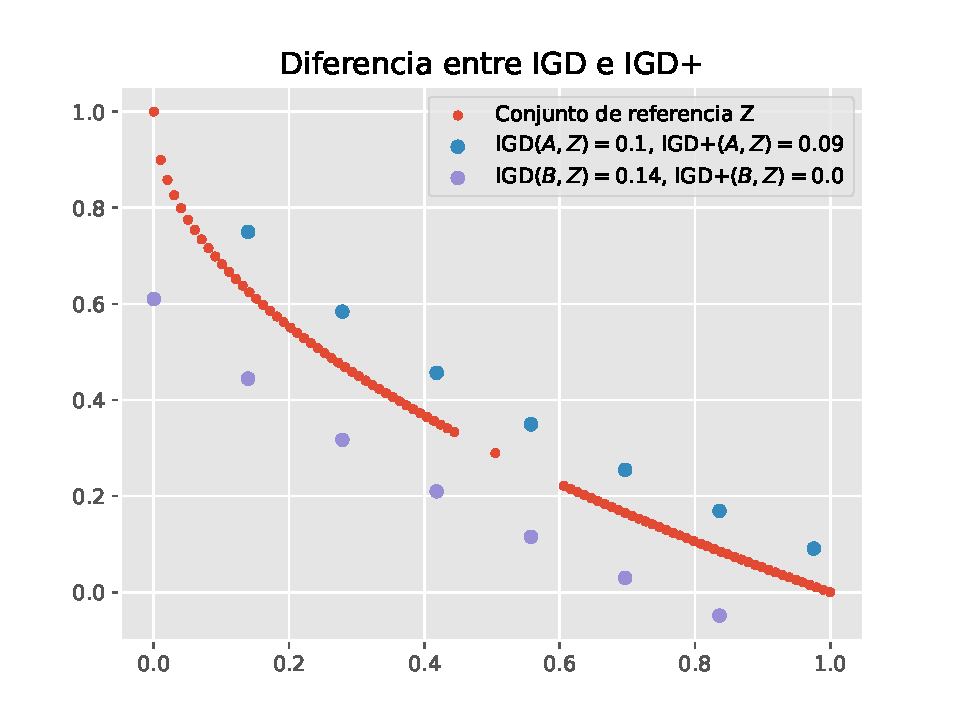
\includegraphics[width=0.8\textwidth]{./Figuras/igdp_demo.pdf} 
    \caption[IGD vs IGD+]{Comparativa entre IGD usual e IGD$+$.}
    \label{fig:comp_IGD_IGDp}
\end{figure}

\subsection{Epsilon +} \label{sec:Epsilonp}
Escrito como $\epsilon_+$ \cite{epsilonplus} es un indicador binario que mide la distancia mínima que habría que recorrer un conjunto $A$ para dominar débilmente al conjunto $B$, la siguiente ecuación describe el cálculo del indicador

\begin{equation} \label{eq:epsp}
    \epsilon_+(A,B)= \max_{b\in B} \min_{a\in A}\max_{j\in 1,\ldots, m} a_j-b_j. 
\end{equation}

Donde $A$ y $B$ son usualmente el conjunto de referencia y el de aproximación. De la Ecuación \ref{eq:epsp} vemos que el indicador depende del orden de los conjuntos.
Para explicar de manera más clara que hace este indicador miremos la Figura \ref{fig:epsp}. Vemos que después de trasladar $A$ por $\epsilon+$ el conjunto $A$ domina al conjunto de referencia. Así, el objetivo de este indicador es minimizar el traslado que hay que hacer para tener similitud entre la referencia y la aproximación. Al requerir un conjunto de referencia, la eficacia del indicador dependerá de si tenemos una buena aproximación al frente de Pareto. 

\begin{figure}[H]
    \centering
    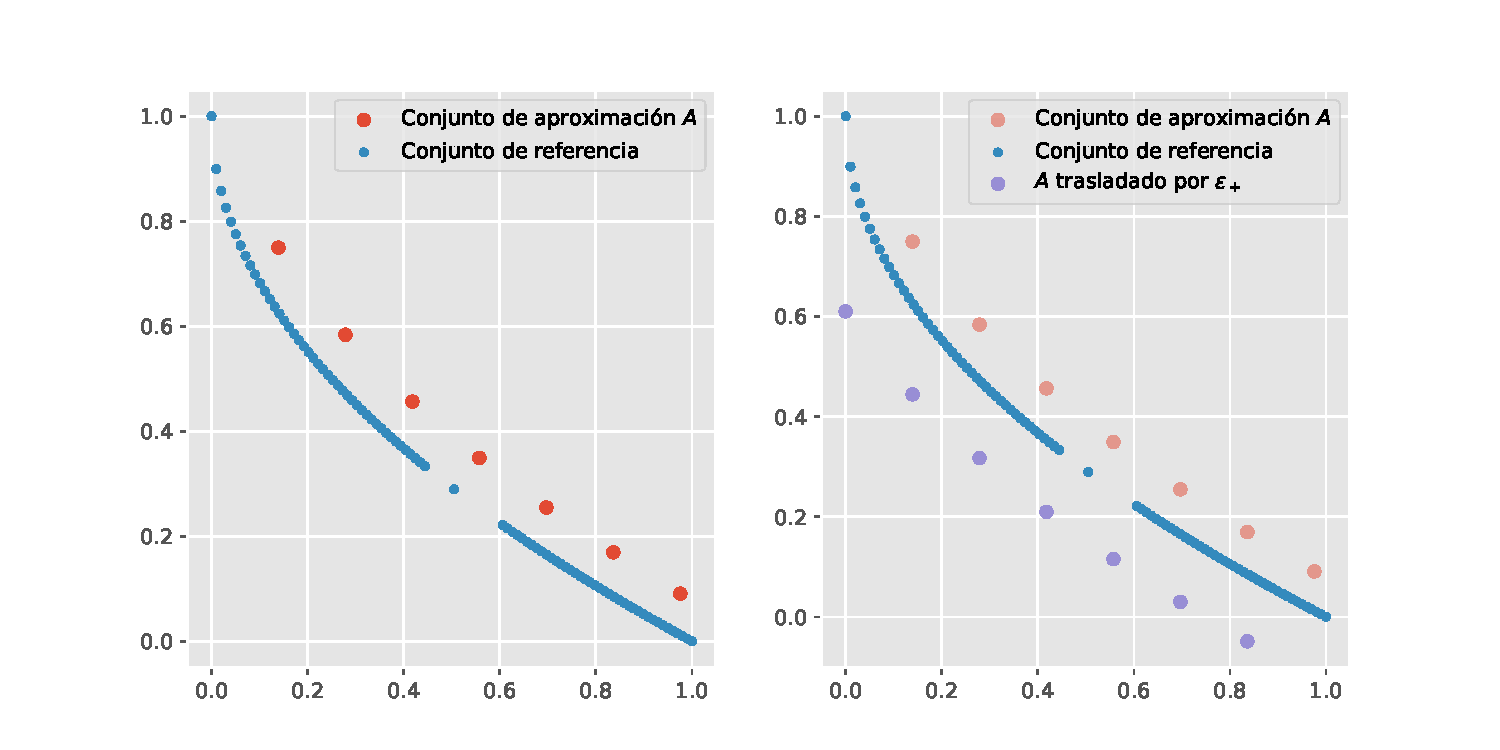
\includegraphics[width=\textwidth]{Figuras/epsilon_plus_demo.pdf}
    \caption[$\epsilon+$]{Ilustración del valor del indicador $\epsilon_+$.}
    \label{fig:epsp}
\end{figure}

\subsection{Diversidad de Solow-Polasky (SPD)} \label{sec:SPD} 
El indicador de diversidad de Solow-Polasky (SPD por sus siglas en inglés) fue originalmente creado en el contexto de biología para medir diversidad de especies y ha sido adaptado para su uso en problemas multiobjetivo. Esto se debe a que satisface propiedades deseables de operadores de diversidad \cite{SPD} como monoticidad en variedades, en distancia y que se mantengan constantes al agregar un elemento que ya esté presente en el conjunto de soluciones.

Dada una población $P = \{P_1, \ldots, P_\mu\}$ de $\mu$ individuos y distancias por pares $d(P_i, P_j)$ para $1 \leq i,j \leq \mu$, Definimos la matriz $M$ de ($\mu \times \mu$) como $M_{ij} = \exp(-\theta  d(P_i, P_j))$. Así, el indicador queda definido por la siguiente ecuación:

\begin{equation} \label{eq:SPD}
    D_{SP}(P) = \sum_{1 \leq i,j \leq \mu} M_{ij}^{-1} \in [1, \mu], \nonumber
\end{equation}


donde $M^{-1}$ es la inversa generalizada de Moore-Penrose de la matriz $M$. Puede ser interpretado como el número de especies diferentes en la población. Su valor cae en los reales entre $1$ y $\mu$ por lo que nos da una medida fina de diversidad. En la Figura \ref{fig:SPD}, podemos ver diferentes valores de SPD para cien puntos distribuidos de diferente manera en el círculo unitario. Vemos que aquellos menos concentrados en el origen reciben mayor SPD. 

\begin{figure}[H]
    \centering
    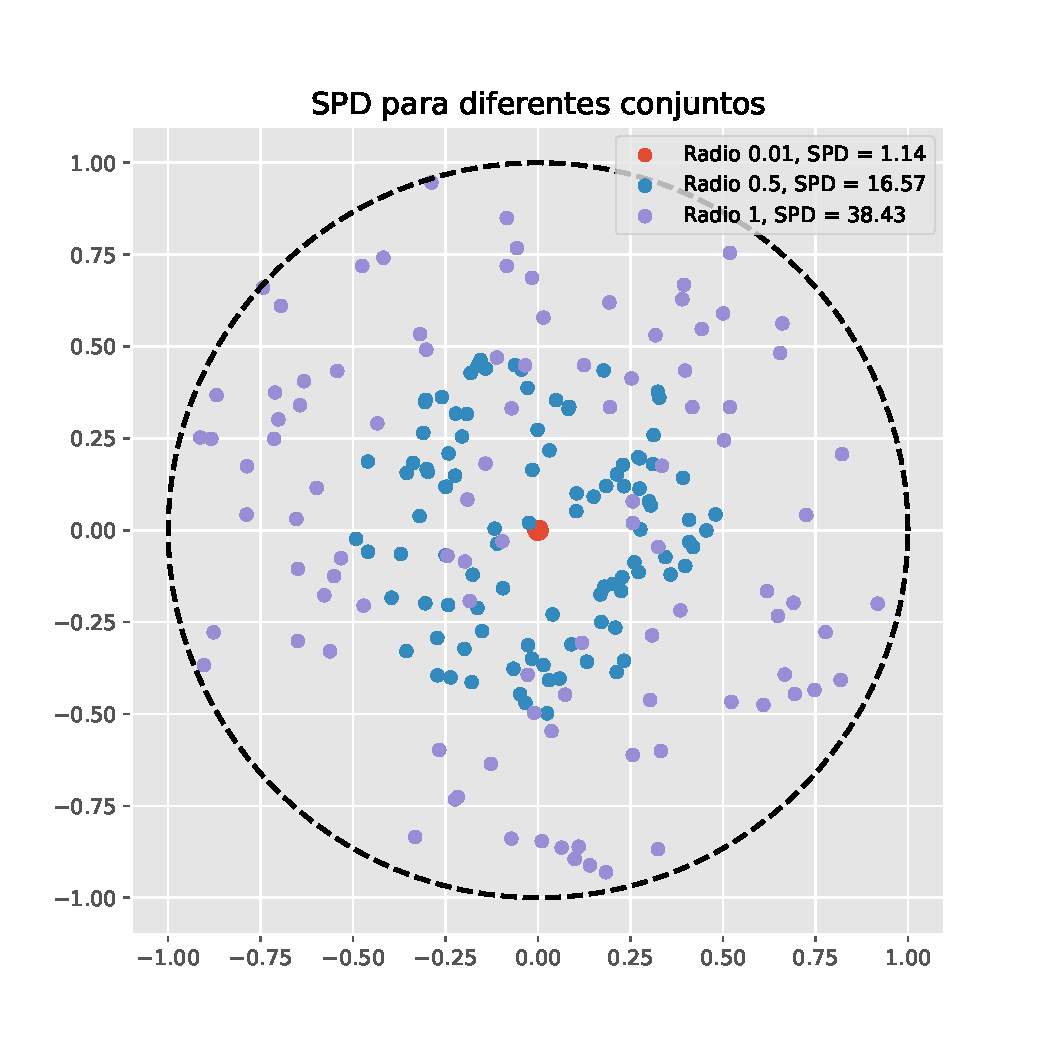
\includegraphics[scale=0.7]{../Figuras/SPD_demo.pdf}
    \caption[SPD]{Valores de SPD para diferentes distribuciones de puntos en el circulo unitario.}
    \label{fig:SPD}
\end{figure}


% The Solow-Polasky diversity indicator is a measure of the diversity of a set of points or solutions, based on a utilitarian model of species conservation². It is defined as the sum of the inverse of the correlation matrix of the points, where the correlation function is exponential⁷. The Solow-Polasky diversity indicator is to be **maximized** to obtain a more diverse set⁷. A higher value of the indicator means that the points are more different from each other and cover a larger area in the space. A lower value means that the points are more similar and clustered together. Therefore, if you want to optimize the Solow-Polasky diversity indicator, you should aim for a **maximal** value.

% Source: Conversation with Bing, 10/21/2023
% (1) A Survey of Diversity Oriented Optimization: Problems, Indicators, and .... https://link.springer.com/chapter/10.1007/978-3-319-49325-1_1.
% (2) indicator — Useful diversity indicators — diversipy 0.7 documentation. https://ls11-www.cs.tu-dortmund.de/people/swessing/diversipy/doc/indicator.html.
% (3) solow_polasky : Solow-Polasky measure - R Package Documentation. https://bing.com/search?q=solow+polasky+diversity+indicator.
% (4) solow_polasky : Solow-Polasky measure - R Package Documentation. https://rdrr.io/github/jakobbossek/ecr3vis/man/solow_polasky.html.
% (5) Diversity-Indicator Based Multi-Objective Evolutionary Algorithm: DI .... https://link.springer.com/chapter/10.1007/978-3-030-12598-1_28.
% (6) Defining and Optimizing Indicator-based Diversity Measures in .... https://bin.re/files/pdf/3.pdf.
% (7) Two-objective solution set optimization to maximize hypervolume and .... https://ieeexplore.ieee.org/document/6505243.

\subsection{R2} \label{sec:R2}
El indicador $R2$ pertenece a un conjunto más general de indicadores conocido como la familia $R$ \cite{R2}. Integra las preferencias del tomador de decisiones mediante una función de densidad de utilidad $h(u)$ y compara un conjunto de aproximación $\mathcal{A}$ con uno de referencia $\mathcal{Z}$ mediante la siguiente ecuación

\begin{equation} \label{eq:R2_completo}
    R2(\mathcal{Z},\mathcal{A},U)=\int_{u\in U} h(u)u^*(\mathcal{Z}) dU- \int_{u\in U} h(u) u^*(\mathcal{Z})du, 
\end{equation}
donde  $u^*(\mathcal{A})$ es el mejor valor que se logra en el conjunto $A$ dado esta función de utilidad. Cuando la información sobre la preferencia del tomador de decisiones no se conoce se puede suponer una función uniforme sobre las funciones de utilidad. Si el conjunto de funciones de utilidad es discreto se puede cambiar la integral por una suma. Además, al comparar el $R2$ de dos conjuntos distintos, podemos ver que el segundo término de \ref{eq:R2_completo} se cancela en la diferencia. De modo que bajo estas características tenemos

\begin{equation} 
    R2(\mathcal{A})=\frac{1}{|W|}\sum_{w\in W} h(u)u(\mathcal{A},w), \nonumber
\end{equation}

$W$ es un conjunto de pesos\\
$h(u)$ es una función de densidad sobre las funciones de utilidad\\
$u(\mathcal{A},w)$ es una función de utilidad.

para la función $u(\mathcal{A},w)$ se pueden usar escalarizaciones comunes como suma ponderada \eqref{eq:suma_ponderada} o la función de escalarización de Tchebycheff \eqref{eq:tchebychev}. Este indicador tiene la ventaja de tener un costo computacional relativamente pequeño, pero tiene menor precisión que otros indicadores que consideran un conjunto continuo de pesos como el IPF. 

% Además cumple con las siguientes características \cite{tesis_phd_guillermo}

% \begin{itemize}
%     \item Es débilmente monótono, i.e.,
% \end{itemize}
% IR2(A)  IR2(B) en caso de que A  B, (2) simultaneamente evalua todos los aspectos
% deseables de una aproximacion al frente de Pareto, (3) las soluciones que genera
% estan usualmente uniformemente distribuidas, y (4) es mucho menos costoso computacionalmente
% que HV.

En este trabajo usamos un conjunto de funciones de utilización conocidas como ASF (Achievement Scalarizing Function) que están dadas en función un conjunto de vectores de pesos convexos\footnote{Los vectores convexos, son no negativos $\lambda_i\geq 0, \forall i$ y suman a uno $\sum_i \lambda_i =1$} $\Lambda$ y un vector de referencia $z$. 

\begin{equation}\label{eq:R2}
    R2(\mathcal{A}, \Lambda, \mathbf{z}) = \frac{1}{|\Lambda|} \sum_{\mathbf{\lambda} \in \Lambda} \max_{\mathbf{a} \in \mathcal{A}} \left\{ \max_{i \in \{1, \ldots, m\}} \lambda_i \left\{ |a_i - z_i|\right\} \right\}
\end{equation}

La región definida por los vectores convexos forman un simplejo en $\mathbb{R}^m$. Los puntos de ese simplejo definirán las funciones de utilidad que evaluamos en \ref{eq:R2}. Existen métodos para distribuir estos puntos como SLD (Simple Latex Desing). En este trabajo usamos un método definido para maximizar la Energía-S de Riesz de los vectores en el simplejo. 

% En la Figura \ref{fig:R2} vemos el cálculo del indicador R2, los vectores de pesos que nos ayudan a materializar las preferencias de la función de utilidad.

% \begin{figure}[H]
%     \centering
%     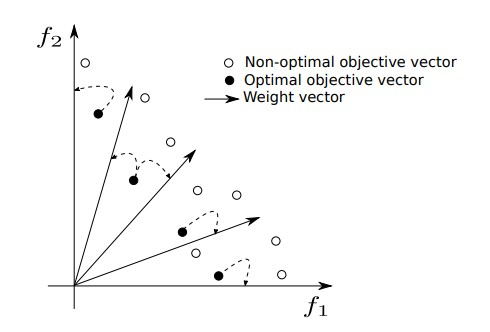
\includegraphics[scale=.6]{./Figuras/R2.jpg} 
%     \caption[R2]{Cálculo de R2. Imagen tomada de \cite{tesis_mst_guillermo}.}
%     \label{fig:R2}
% \end{figure}

% The R2 indicator is a measure of the quality of a set of solutions in multiobjective optimization, based on a utilitarian model of species conservation². It is defined as the weighted sum of the hypervolumes of the scalarized optimization problems⁶. The R2 indicator is to be **maximized** to obtain a better set of solutions⁴⁵. A higher value of the R2 indicator means that the solutions are more optimal and diverse, and cover a larger portion of the Pareto front. A lower value means that the solutions are less optimal and diverse, and cover a smaller portion of the Pareto front. Therefore, if you want to optimize the R2 indicator in multiobjective optimization, you should aim for a **maximal** value.

% Source: Conversation with Bing, 10/21/2023
% (1) . https://bing.com/search?q=R2+indicator+in+multiobjective+optimization.
% (2) undefined. https://arxiv.org/abs/2305.11774.
% (3) R2-IBEA: R2 indicator based evolutionary algorithm for multiobjective .... https://ieeexplore.ieee.org/document/6557783/.
% (4) R2-EMOA: Focused Multiobjective Search Using R2-Indicator-Based Selection. https://inria.hal.science/hal-00807901/document/.
% (5) A new weight vectors generation method for R2 indicator based .... https://ieeexplore.ieee.org/document/7979300/.
% (6) Multi-objective particle swarm optimization with R2 indicator and .... https://link.springer.com/article/10.1007/s40747-021-00445-3.
% (7) undefined. https://ieeexplore.ieee.org/servlet/opac?punumber=6552460.

\subsection{Energía S} \label{sec:Energía-S}
La Energía-S de Riesz \cite{sEnergy} es una medida de la uniformidad de soluciones que depende de un parámetro $s$. Está basada en que la energía potencial entre dos cuerpos va como el inverso de su distancia.  Tiene la ventaja de no necesitar un conjunto de referencia, es decir, es un operador unario y está dada por 

\begin{equation} \label{eq:S_energy}
    E_s(A)=\sum_{i\neq j} ||a_i-a_j||^{-s},
\end{equation}
mientras $s\rightarrow \infty$ la Energía-S de Riesz tiende a soluciones más uniformes. Además, el parámetro $s$ es independiente de la forma y ha sido usado para producir conjuntos uniformemente distribuidos en una clase grande de variedades $d$-dimensionales rectificables.

% Conjuntos con diferente energía S comparados con conjuntos con diferente SPD. 



\subsection*{Contribución de solución al indicador}
Para la siguiente sección también será útil definir la contribución de una solución a un cierto indicador; es decir, que tan importante es la solución particular para el desempeño de la solución. Eso es útil porque podemos distinguir cuál es la solución que menos ayuda a optimizar un indicador dado. De manera más formal usamos la Ecuación \eqref{eq:Contribucion}. Esta mide el efecto de quitar un punto en el cálculo del indicador y ver su efecto. Si $a$ es un punto que ayuda mucho a elevar el indicador, entonces $I(A)$ será muy diferente a $I(A \setminus \{a\})$.

\begin{equation} \label{eq:Contribucion}
    C_I(a,A)=|I(A)-I(A \setminus \{a\}) |.
\end{equation}


\section{Taxonomía de EMOAs} \label{sec:QIs_tax}

En esta sección se revisa una clasificación de EMOAs además de dar un ejemplo de cada uno de ellos. Las categorías que se revisan son: 

\begin{itemize}
\item No-Elitistas no-basados en optimalidad de Pareto. Poniendo como ejemplo a VEGA \cite{schafferMultipleObjectiveOptimization1984}.
\item No-Elitistas basados en dominancia de Pareto. Poniendo como ejemplo a NSGA \cite{debFastElitistNondominated2000}.
\item Elitistas basados en dominancia de Pareto. Poniendo como ejemplo a NSGA-II \cite{seifbarghyNovelMetaheuristicAlgorithm2016}.
\item EMOAs basados en indicadores. Poniendo como ejemplo a SMS-EMOA \cite{SMS-EMOA}.
\end{itemize}


\subsection*{No-Elitistas no-basados en optimalidad de Pareto} \label{sec:VEGA}

Para ejemplificar esta clase de algoritmos explicaremos el primer EMOA propuesto por Schaeffer \cite{schafferMultipleObjectiveOptimization1984} llamado VEGA (Vector Evaluation Genetic Algorithm). Este algoritmo consiste en dividir la población total de $M$ individuos en subpoblaciones y hacer que cada uno de ellos evolucionara para resolver uno de los $k$ objetivos en un algoritmo no-elitista. Después en la siguiente generación, se revolvían de manera aleatoria los individuos y se volvían a dividir en subpoblaciones para atacar cada uno de los objetivos que, para cada individuo, podría ser un objetivo distinto al que se le había asignado previamente, podemos ver una representación en la Figura \ref{fig:VEGA}, adaptada de \cite{coelloEvolutionaryAlgorithmsSolving}.

\begin{figure}[H]
    \centering
    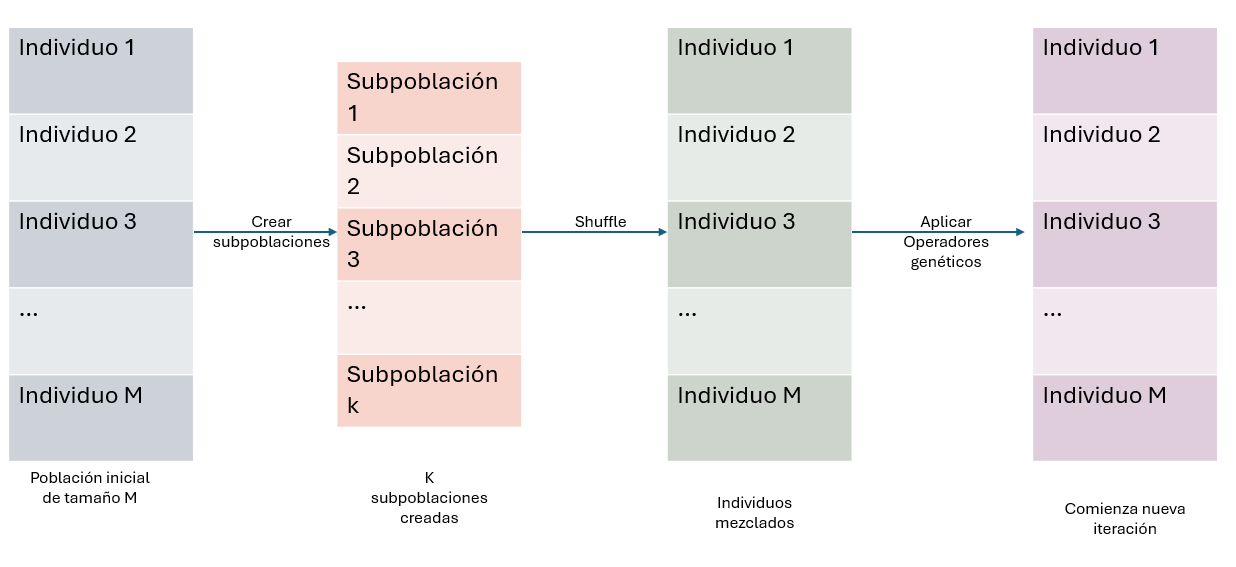
\includegraphics[width=\textwidth]{Figuras/VEGA_diagrama.png}
    \caption[VEGA]{Ilustración del algoritmo de VEGA.}
    \label{fig:VEGA}
\end{figure}

Este algoritmo presentó problemas para encontrar diversidad y para encontrar soluciones que realmente no fueran óptimas de Pareto. Además, el enfoque de cada subpoblación en objetivos llevó a lo que Schaeffer llamó especiación, en el que se seleccionan individuos que son muy buenos para una tarea y malos para las demás, de modo que se obtiene un desempeño aceptable, pero no excelente. Este algoritmo no integra específicamente la dominancia de Pareto por lo que se puede clasificar como uno \textbf{No elitista no basado en optimalidad de Pareto}.

\subsection*{No-Elitistas basados en dominancia de Pareto}

Para ejemplificar este tipo de algoritmos se describirá brevemente uno de los más importantes dentro de esta categoría, NSGA. En 1994 se presentó el algoritmo Nondominated Sorting Genetic Algorithm \cite{srinivasMuiltiobjectiveOptimizationUsing1994} que ataca directamente el problema de obtener soluciones no dominadas mediante una clasificación de capas de subpoblaciones. Se realiza un procedimiento iterativo en el que se seleccionan los individuos que no estén dominados y se les asigna un ranking de 1, después se quitan estos individuos de la población y se repite el procedimiento hasta agotar los individuos incrementando el ranking en cada capa, como se puede ver en la Figura \ref{fig:nsga1}.

\begin{figure}[H]
    \centering
    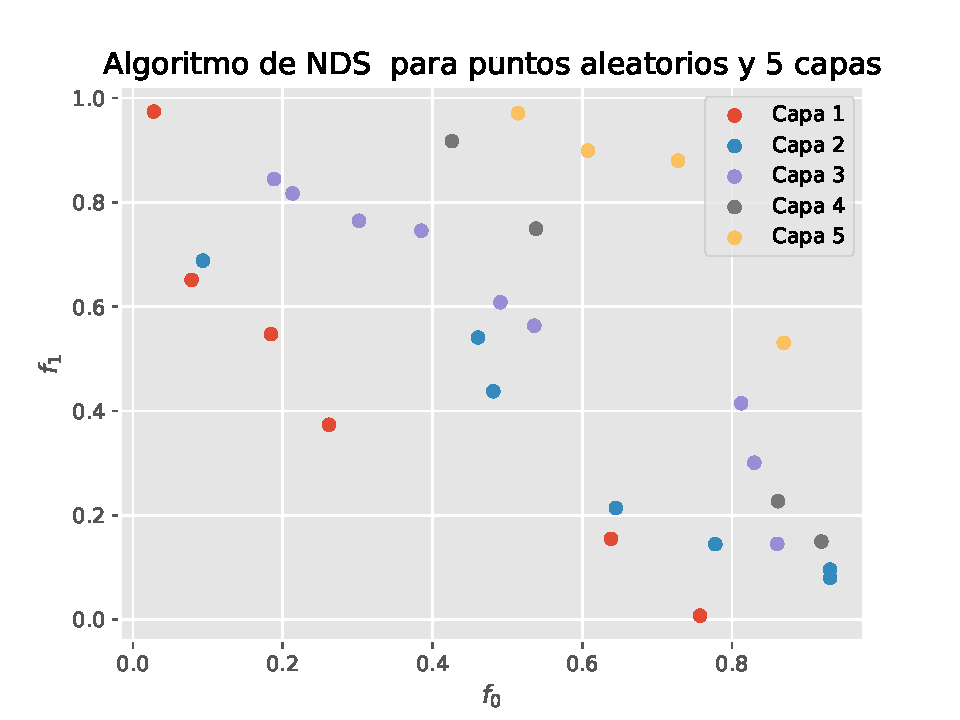
\includegraphics[width=\textwidth]{Figuras/nds.pdf}
    \caption[NSGA]{Capas del algoritmo de NSGA. Primero se encontrarían aquellos que están etiquetados como rank 1, se quitarían de la población y así sucesivamente.}
    \label{fig:nsga1}
\end{figure}

% ¿Hace Falta poner algoritmo?

Este algoritmo también es no-elitista lo que hace muy costoso el cálculo de los rankings en cada una de las generaciones por lo que se le llama un algoritmo \textbf{No-elitista basado en optimalidad de Pareto}.

\subsection*{Elitistas basados en dominancia de Pareto.} \label{sec:nsga2}

Para ejemplificar este tipo de algoritmos se explica brevemente el funcionamiento del algoritmo NSGA-II.  

En el 2000 se publicó \cite{debFastElitistNondominated2000} una actualización del algoritmo anterior que ataca el problema de la complejidad computacional y el de la diversidad de las soluciones proponiendo dos mecanismos diferentes. Para el problema de la complejidad ahora se usa un enfoque elitista. De esta forma se pueden conservar rankings de generaciones anteriores y no se tiene la carga computacional de estarlos calculando constantemente. Además de esto para asegurar que los individuos de una población no se concentran en una región pequeña del espacio, se suelen usar algún \textbf{estimador de densidad} que mide que tan cerca están los puntos y puede lograr que no existan demasiados aglomerados en una región pequeña del espacio. En NSGA-II se usa un estimador de densidad llamado \textbf{crowding distance} en su operador de selección para calcularlo, primero se ordenan los valores de los objetivos en cada una de las direcciones. A los puntos extremos en este ordenamiento se les asigna una distancia infinita porque no se quiere que se eliminen de la población. Para el individuo $i$-ésimo se realiza el siguiente cálculo

\begin{equation} \label{eq:crowding_distance}    
    \text{crowding distance} (d_i) = \sum_{m=1}^M \left( \frac{f_m^{(i+1)} - f_m^{(i-1)}}{f_m^{\text{max}} - f_m^{\text{min}}} \right)
\end{equation}

donde:
\begin{itemize}
    \item \(d_i\) es la \text{crowding distance} para el individuo \(i\).
    \item \(M\) es el número de objetivos.
    \item \(f_m\) representa la función objetivo \(m\).
    \item \(f_m^{(i+1)}\) y \(f_m^{(i-1)}\) son los valores de la función objetivo \(m\) de los individuos adyacentes a \(i\) en la lista ordenada.
    \item \(f_m^{\text{max}}\) y \(f_m^{\text{min}}\) son los valores máximos y mínimos de la función objetivo \(m\) entre todos los individuos.
\end{itemize}

Este operador mide el perímetro del cuadrado que separa a una solución de sus vecinos más cercanos en todas direcciones, como podemos ver en la Figura \ref{fig:crowding_distance}.  Cuando existe algún empate en el rango de dos soluciones, la solución que tenga mayor crowding distance es preferida. De este modo se promueve que la densidad de las soluciones sea menor y esto ayuda a la diversidad de la población. 

\begin{figure}[H]
    \centering
    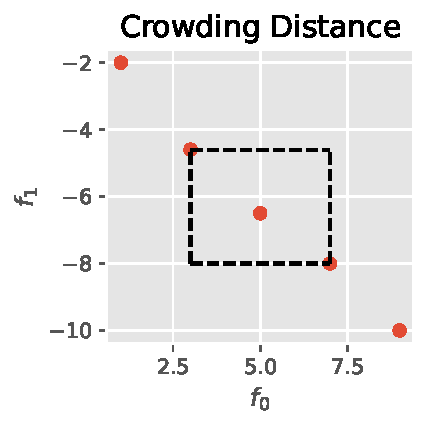
\includegraphics[scale=1]{./Figuras/crowding_distance.pdf}
    \caption{Vemos el rectángulo con el que se calcula la crowding distance de la solución de enmedio.}
    \label{fig:crowding_distance}
\end{figure}

\begin{algorithm}
    \caption{Algoritmo NSGA-II}
    \begin{algorithmic}[1]
    \setlength{\itemsep}{1pt} % Set the spacing between items
\setlength{\parskip}{0pt} % Set paragraph spacing to zero
    \State $P_0 \gets \text{InicializarPoblación()}$
    \State $t \gets 0$
    \While{\text{Criterio de Terminación NO CUMPLIDO}}
        \State $Q_t \gets \text{OperacionesGenéticas}(P_t)$
        \State $R_t \gets P_t \cup Q_t$
        \State $\{F_1, F_2, \ldots\} \gets \text{NDS}(R_t)$
        \State $P_{t+1} \gets \text{vacío}$
        \State $i \gets 1$
        \While{$|P_{t+1}| + |F_i| \leq N$}
            \State $\text{CrowdingDistance}(F_i)$
            \State $P_{t+1} \gets P_{t+1} \cup F_i$
            \State $i \gets i + 1$
        \EndWhile
        \State $F_i \gets \text{Ordenar}(F_i, \text{por: CrowdingDistance, desc})$
        \State $P_{t+1} \gets P_{t+1} \cup F_i[1:(N - |P_{t+1}|)]$
        \State $t \gets t + 1$
    \EndWhile
    \end{algorithmic}
\end{algorithm}

Este algoritmo ha sido muy exitoso siendo la referencia contra la que se comparan la mayoría de las propuestas de EMOAs. Su capacidad exploratoria es cuestionable, parece tener dificultad generando soluciones no dominadas en regiones aisladas como cuando se incrementa el número de dimensiones \cite{coelloEvolutionaryAlgorithmsSolving}. Por sus características se le conoce como un algoritmo \textbf{Elitista basado en dominancia de Pareto}.

Existen muchos otros EMOAs además de los que hemos hablado en esta sección, sin embargo, con los ya expuestos basta para motivar y definir el algoritmo que usaremos en este trabajo. Para eso, la siguiente sección revisa el concepto de indicadores de calidad para aproximaciones al frente de Pareto. 

\section{Métodos basados en indicadores de calidad} \label{sec:Metodos_QI}

Al igual que en muchos problemas que lidian con dimensiones altas, los algoritmos multiobjetivo sufren de efectos de escalamiento al aumentar las dimensiones del espacio. Es decir, el problema de ir incrementando las dimensiones no requiere solamente cambiar parámetros en una función, sino que requiere de una manera distinta de abordar el problema.
Para lograr una buena cobertura del Frente de Pareto, el número total de puntos (soluciones) necesarios escala exponencialmente con el número de funciones objetivo, lo que hace que muchos enfoques existentes sean inviables a medida que aumenta la dimensionalidad del espacio objetivo \cite{tanParetoOptimizationSmall2023}. 

Esto se debe, en el caso de algoritmos multiobjetivo, a que un algoritmo podrá generar con facilidad un conjunto que no esté dominado con respecto a otro sin que esto haga que los puntos necesariamente se aproximen al frente de Pareto. De acuerdo a lo visto en la Sección de dominancia de Pareto \ref{sec:Dominancia_Pareto}, el espacio de estados que dominan a un punto dado en el espacio de objetivos corresponde a aquellos que están en el cuadrante $--$ que, como su nombre lo indica, cubre un cuarto de todo el espacio. Incrementando la el número de objetivos, ahora tenemos más combinaciones de signos que no están mutuamente no dominados, como podemos observar en la Figura \ref{fig:maldicion_dim} donde tenemos en la primera figura de la izquierda el cuadrante de región dominada desde el origen. Después, en la de en medio, el octante en para tres objetivos y finalmente vemos una curva de cuánto espacio ocupa la región dominada por el origen mientras incrementamos el número de objtetivos. Al ser el número de dimensiones más grande, nuestro algoritmo puede pasar mucho tiempo buscando en el espacio de estados que no llevan a una aproximación cada vez mejor del frente real de Pareto. 

\begin{figure}[H]
    \centering
    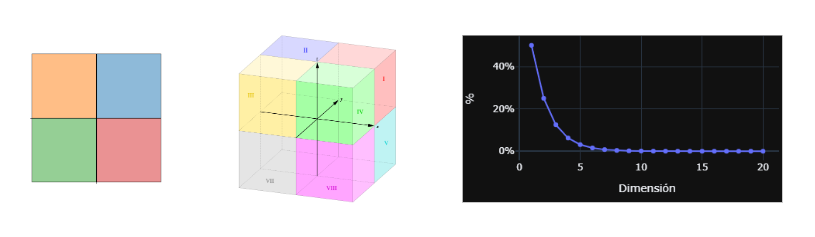
\includegraphics[width=\textwidth]{Figuras/maldicion_dimensionalidad.png}
    \caption[maldicion de la dimensionalidad]{Dimensionalidad y región dominada.}
    \label{fig:maldicion_dim}
\end{figure}

Una manera de resolver este problema es reducir la dimensión del espacio objetivo de los problemas estudiados, este enfoque se puede seguir usando escalarizaciones o definiendo cantidades útiles, esto último es lo que pretenden hacer los indicadores de calidad que definiremos en esta sección. Como mencionamos en la Sección \ref{sec:QIs}, los indicadores de calidad son propiedades de los conjuntos de soluciones que resumen sus características en valores que expresan, por ejemplo, qué tan separados están los individuos, cuántos individuos hay, qué tanto rango abarcan, qué tan cerca están de converger a un conjunto de referencia, qué tan uniformemente están separados, etc. Los indicadores no se usan explícitamente para reducir las dimensiones del problema; es decir, encontrando el frente de Pareto en el espacio de los indicadores, sino que se usa esta información a mayor nivel de la aproximación para tomar decisiones acerca de, por ejemplo, que solución mantener en caso de un empate. Los Indicadores de calidad también son importantes para comparar algoritmos, ya que, como veremos a continuación, es difícil saber cuándo una aproximación al frente de Pareto es mejor a otra. 

\subsection*{SMS-EMOA} \label{sec:SMS-EMOA}

Habiendo definido los indicadores y los algoritmos previos, en esta sección describiremos uno de los primeros IB-EMOAs llamado S Metric Selection-EMOA (SMS-EMOA) \cite{SMS-EMOA}. Este algoritmo es muy parecido a aquel de NSGA-II, que revisamos en la Sección \ref{sec:nsga2}, ya que también es no-elitista y usa non-dominated sorting. Sin embargo, en vez de usar el estimador de densidad basado en crowding distance utiliza un indicador de hipervolumen, además de esto es un algoritmo que cae en una familia de AE conocidos como steady-state. Esto significa que solamente se genera un hijo en cada una de las evaluaciones de la función de selección; es decir, es un algoritmo $\mu+1$. Se realiza de esta manera ya que, al usar el HV, se tiene que encontrar el individuo que menos contribuye en su maximización de toda la población de tamaño $N$. Así, se usa la Ecuación \eqref{eq:Contribucion} para iterar sobre los individuos y escoger el que se eliminará en la siguiente generación. Si se quedaran dos individuos nuevos, entonces habría que hacer $\binom{N}{2}=\frac{N(N-1)}{2}=O(N^2)$ comparaciones de modo que el algoritmo se volvería muy costoso. En el Algoritmo \ref{alg:SMS-EMOA} podemos ver el pseudocódigo de SMS-EMOA.

\begin{algorithm}
    \caption{SMS-EMOA}\label{alg:SMS-EMOA}
    \begin{algorithmic}[1] % The number indicates line numbering step
        \State $P_0$ = init;
        \State $t_0$ = init;

        \Repeat
        
        $q_{t+1}$ = genera($P_t$)
        
        $\{\mathcal{R}_1,\ldots,\mathcal{R}_v\}$ =fast-nds($P_t \cup \{q_{t+1}\})$
        
        $r=\text{argmin}_{S\in \mathcal{R}_v}\left( \text{HV}(s,\mathcal{R_v}) \right)$
        
        $P_{t+1}= Q \setminus \{r\}$;
        
        $t=t+1$;
        
        \Until condicion de termino

    \end{algorithmic}
\end{algorithm}

Este algoritmo es bueno en tareas que NSGA-II no lo era, como aumentando el número de objetivos hasta 4. El cálculo del HV para dimensiones mayores se vuelve costoso computacionalmente y, como se mencionó anteriormente, el cálculo es dependiente de la elección del punto de referencia. Esto puede afectar la diversidad y convergencia de las soluciones obtenidas.

Se han hecho muchos IB-EMOAs que, al igual que SMS-EMOA sólo utilizan uno de ellos para guiar su exploración y explotación del espacio de estados. Por lo tanto, heredan las virtudes y los defectos de depender tanto de una cualidad del conjunto de soluciones que se va generando, o del conjunto de referencia del frente de Pareto. Por ejemplo, los basados en HV generan muchas soluciones alrededor de la \emph{rodilla} y las fronteras del frente de Pareto, mientras que producen soluciones bien distribuidas para frentes convexos y lineales, además de tener buen desempeño en frentes degenerados \cite{HV_reference}, \cite{SMS-EMOA}. Los que están basados en R2, visto en la Sección \ref{sec:R2}, tienen buena distribución en frentes cóncavos, pero no hacen lo mismo para frentes convexos, degenerados o desconectados, dado a que los vectores de peso convexos intersectan esas geometría \cite{performance_pareto_front}, \cite{R2-EMOA}. Por esta razón, una extensión natural a los IB-EMOAs de un indicador, es usar varios indicadores para que sus objetivos estén en contraste, que puedan evitar problemas de sobre-especialización y que no sean dependientes de la forma del frente de Pareto.  

\section{PFI-EMOA} \label{sec:PFI-EMOA}

En esta sección se detalla el algoritmo usado en este trabajo. Recibe el nombre de Pareto Front Invariant EMOA (PFI-EMOA) y nace de la necesidad de encontrar un algoritmo que funcione para muchas dimensiones y a la vez que no tenga las restricciones mencionadas en el último párrafo de la sección anterior. La idea principal de este algoritmo es seguir con el marco principal de SMS-EMOA; es decir, usar non-dominated sorting para rankear las soluciones y usar un algoritmo steady-state para no hacer muchas comparaciones de contribuciones a indicadores. La diferencia principal es que se reemplaza el estimador de densidad de Hipervolumen que estaba presente en SMS-EMOA por una combinación de dos indicadores: IGD+ \eqref{eq:IGDp} y la Energía-S de Riesz \eqref{eq:S_energy}. Al ser estos dos indicadores de categorías diferentes (convergencia principalmente y diversidad) tendrán objetivos conflictuantes que obligarán a explorar una región distinta del espacio de estados. Estos dos indicadores se combinan por medio de la función aumentada de Tchebycheff,  qeue para un vector $\vec{x}=(x_0,x_1)$ está dada por


\begin{equation} \label{eq:ATCH}
    \text{ATCH}_{\vec{w}}(x_0,x_1)=\max_{i=0,1} \{w_ix_i\}+\alpha (x_0+x_1),  
\end{equation}


Sustituyendo cada uno de los indicadores tenemos
\begin{align*}
    \text{ATCH}_{\vec{w}}=({\text{IGD}}^+(A,Z),E_s(A)), \nonumber
\end{align*}

% \begin{align} \label{eq:ATCH}
%     \text{ATCH}_{\vec{w}}({\text{IGD}}^+(A,Z),E_s(A))=&\max \{w_0{\text{IGD}}^+(A,Z),w_1E_s(A)\}\\&+\alpha ({\text{IGD}}^+(A,Z)+E_s(A))
% \end{align}

donde $Z$ es un conjunto de referencia y $A$ es la aproximación al frente de Pareto.

Una característica interesante de hacer esta combinación es que se obtiene un indicador que no es consistente de Pareto. Esto se debe a un teorema probado en \cite{falcon-cardonaConstructionParetoCompliantCombined2022} que asegura que si se combina un indicador débilmente consistente de Pareto (IGD+) \eqref{eq:consistente_debil_Pareto} con uno que no lo es (Energía-S), entonces se tendrá como resultado uno que no es consistente de Pareto. Entonces se deben analizar los tres casos de la Figura \ref{fig:casos} como si fuera un problema de dominancia usual en dos dimensiones.

\begin{figure}[H]
    \centering
    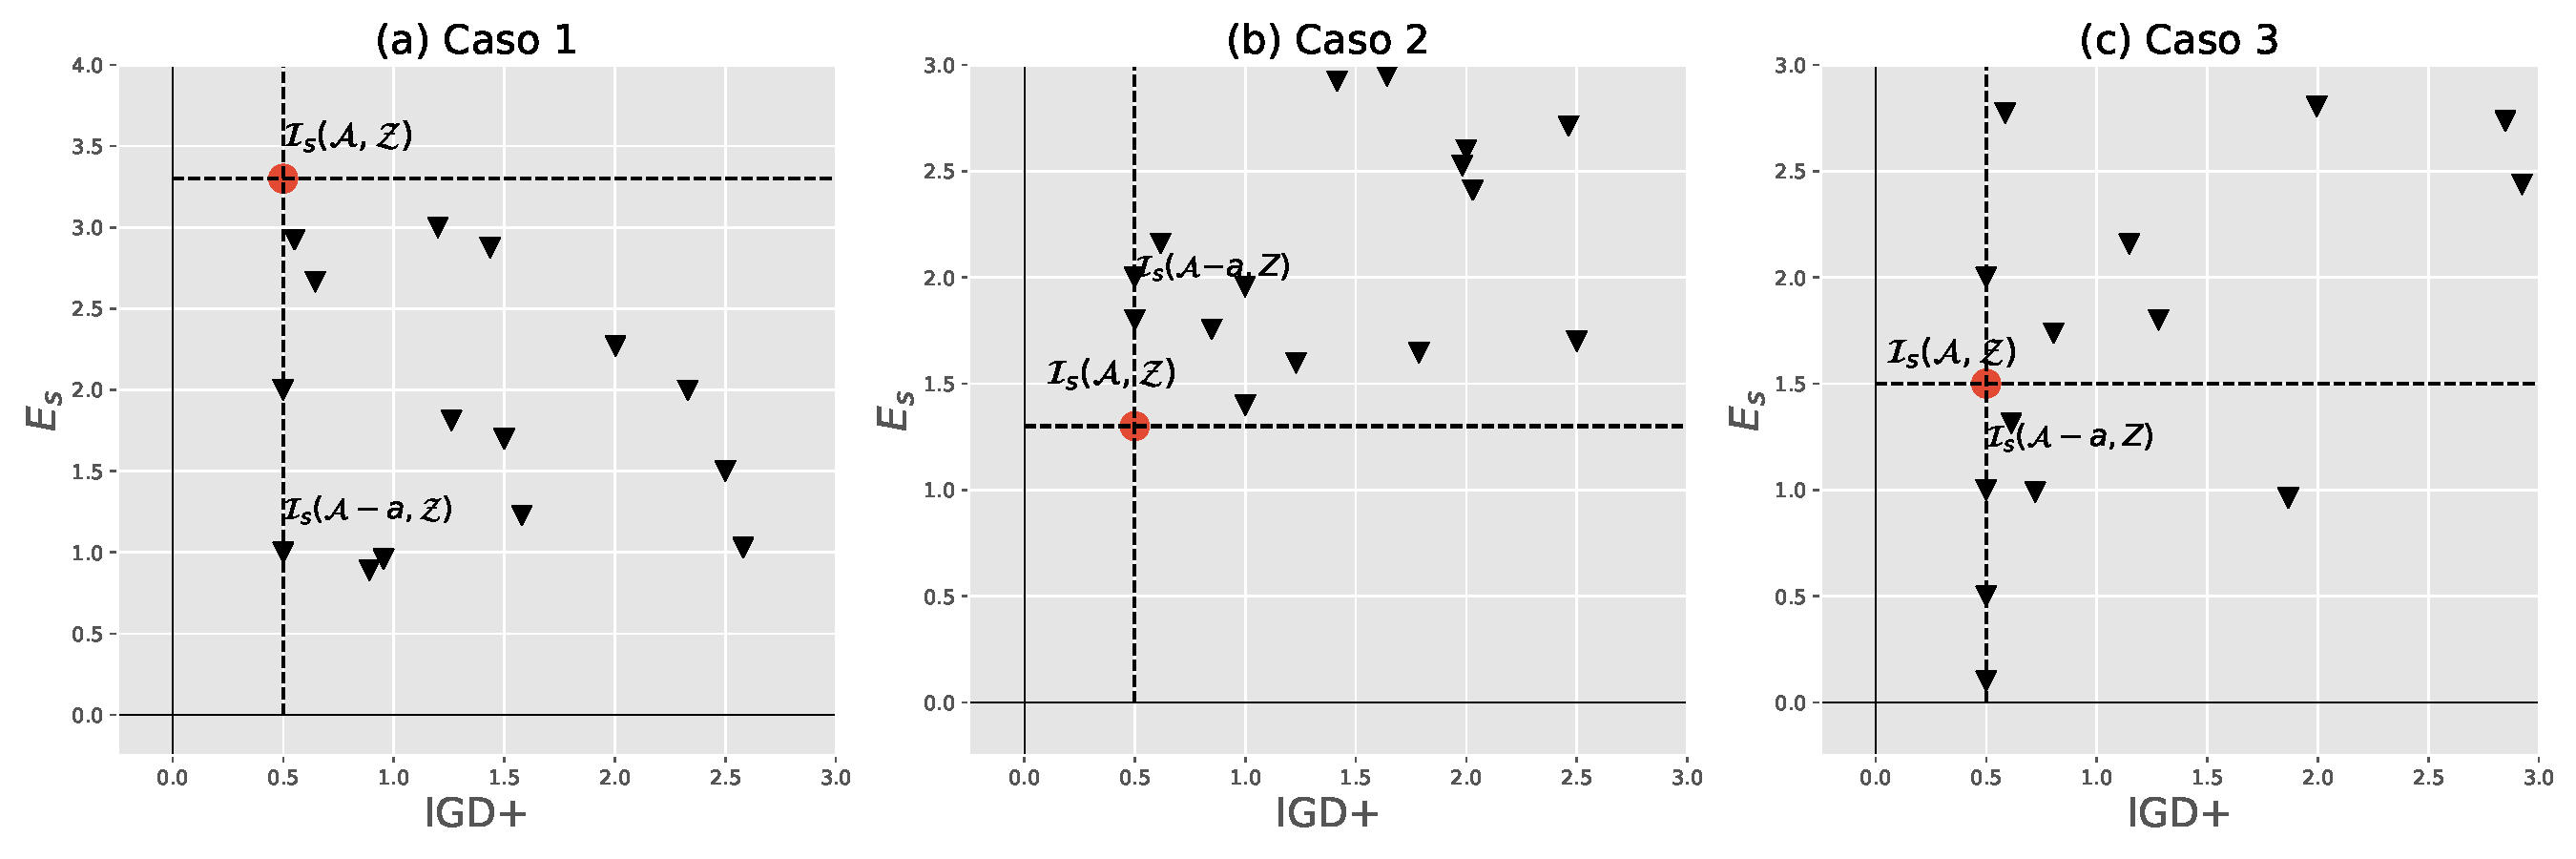
\includegraphics[width=\textwidth]{Figuras/casos.pdf}
    \caption[Tres casos para PFI.emoa]{Tres casos de selección diferentes dependiendo del comportamiento de la contribución al indicador combinado \eqref{eq:Contribucion}.}
    \label{fig:casos}
\end{figure}


En el caso 1, cada que una solución se remueve de $A$, $E_s$ se vuelve mejor. Entonces $\vec{I}_s(A,Z)$ está mutuamente no dominado contra las contribuciones de cada solución, $\vec{I}_s(A \setminus {\vec{a}},Z)$. Entonces $\text{ATCH}$ podría ser menor, igual o mayor antes y después de quitar la solución $\vec{a}$. En el caso 2, todos los vectores  $\vec{I}_s(A \setminus {\vec{a}},Z)$ están dominados por  $\vec{I}_s(A ,Z)$ por tener $E_s$ mayor, dado que $\text{ATCH}$ preserva orden\footnote{Esto quiere decir que $\text{ATCH}(\vec{I}_s(A,Z))< \text{ATCH}(\vec{I}_s(A \setminus {\vec{a}},Z))$}. Finalmente el caso 3 es una combinación de ambos. Como existe una solución que no contribuye a la convergencia del algoritmo, en cualquiera de estos 3 casos, se elimina la solución que peor contribuya a la Energía-S. En el Algoritmo \ref{alg:PFI-EMOA} podemos ver el pseudocódigo de PFI-EMOA.


\begin{algorithm}
    \caption{PFI-EMOA}\label{alg:PFI-EMOA}
    \begin{algorithmic}[1] % The number indicates line numbering step
        \Require Vector de pesos $\vec{w}\in \mathbb{R}^2$ 
        \Ensure  Aproximación del Frente de Pareto
        \State $P_0$ = init;

        \Repeat
                
        $q_{t+1}$ = genera($P_t$)
        
        $\{\mathcal{R_1},\ldots,\mathcal{R}_k\}$ =fast-nds($P_t \cup \{q_{t+1}\})$
        
        \If{$|R_k|>1$}  

        \State $z_i^{\max} = \max_{\vec{a}\in Q} a_i, i=1,\ldots,m$
        \State $z_i^{\min} = \min_{\vec{a}\in Q} a_i, i=1,\ldots,m$

        Normalizar $\{R_j\}_{j=1,\ldots,k}$ usando $\vec{z}^{\max}, \vec{z}^{\min}$

        \State $B = \{\vec{b} \ |\  \text{IGD}^+(\mathcal{R}_k \setminus \{\vec{b}\})=\text{IGD}^+(\mathcal{R}_k,\mathcal{R}_1), \forall \vec{b} \in \mathcal{R}_k\}$
        \If{$|B|>0$}
        $\vec{a}_{\text{worst}}=\text{argmax}_{\vec{b}\in B} C_{E_s}(\vec{b},\mathcal{R}_k)$ 
        \Else 
        
        $\vec{a}_{\text{worst}}=\text{argmax}_{\vec{r}\in \mathcal{R}_k} \text{ATCH}_{\vec{w}}(\vec{I}_s(\mathcal{R}_k \setminus \{r\}),\mathcal{R}_1)$ 
        
        

        \EndIf

            \Else 

            $\vec{a}_{\text{worst}}$ es la única solución de $\mathcal{R}_k$
        \EndIf 

        $P=Q\setminus \{\vec{a}_{\text{worst}}\}$
     
        
        \Until condicion de termino

    \end{algorithmic}
\end{algorithm}

Iremos explicando este algoritmo línea por línea. Al inicio se requiere como parte de la entrada un vector de pesos. Esto será importante ya que en \cite{PFI} sólo se usó una combinación fija de pesos para una serie de problemas prueba (revisaremos estos problemas en el próximo capítulo). Enseguida, ya entrando en el algoritmo se inicializa la población en la línea 1 y se comienza un ciclo en la línea 2 hasta cumplir la condición de término . En este trabajo la condición de paro se estableció como las iteraciones necesarias para superar un número fijo de generaciones. Las siguientes dos líneas sin número abajo de \textbf{repeat} generan un hijo a través de operadores evolutivos y abajo se utiliza non-dominated sorting para rankear las soluciones, como en la Figura \ref{fig:nsga1}, siendo $\mathcal{R}_k$ las soluciones de la peor capa. 
Siguiendo con la línea 3, entramos al \textbf{if} que nos pregunta si existe más de una solución en la última capa, si la hay, entonces hay que usar el estimador de densidad que se desglosa en varios casos. Primero, en las líneas 4 y 5 se normaliza el rango de los objetivos dividiendo entre el máximo y el mínimo de cada dimensión. Después, en la línea 6 se construyen los diferentes casos que corresponden a la Figura \ref{fig:casos}. Primero, vemos el conjunto de soluciones que no contribuyen al indicador de $\text{IGD}^+$, si tiene más de una solución, se elimina aquella con peor contribución a la Energía-S de Riesz. En caso contrario se usa el estimador de densidad dado por la función aumentada de Tchebycheff \eqref{eq:ATCH}. Finalmente, vemos el caso donde la última capa sólo tuvo un elemento, entonces no hay que escoger cuál eliminar porque solo hay un candidato. En la penúltima línea se actualiza la población quitando la peor solución $\vec{a}_{\text{worst}}$ y se revisa si se alcanzó la condición de término para regresar la aproximación al frente de Pareto. 

\section{Pruebas Estadísticas y Comparación de algoritmos} \label{sec:pruebas_estadisticas}

El interés principal de este trabajo es el de comparar el desempeño de distintas configuraciones de pesos en el algoritmo \ref{sec:PFI-EMOA}. Para fines prácticos, esto se puede entender como comparar el desempeño de algoritmos distintos. Así, planteareamos de manera general cómo se pueden comparar un conjunto de algoritmos que dan un resultado distinto para las mismas entradas\footnote{Estas entradas corresponden a las poblaciones iniciales y pueden ser comparadas entre sí porque se generan usando semillas aleatorias.}. Dado que los EMOAs tienen un comportamiento estocástico, tendremos que hacer muchas corridas de los algoritmos y comparar poblaciones de resultados entre sí. Es por ello que recurriremos a pruebas estadísticas para determinar si el desempeño de los algoritmos fue distinto. La manera en la que decidiremos si un algoritmo tuvo mejor desempeño que otro es usando nuevamente los inidcadores de calidad, pero ahora calculandolos sobre la población final (recordando que la salida de los EMOAs son conjuntos de aproximación al frente de Pareto).

Entonces, por cada población final, haremos el cálculo de cada uno de los indicadores que están en \ref{sec:AE} para cada corrida de cada algoritmo y los compararemos usando las pruebas estadísticas que se exponen en esta sección. Al ser muchos los indicadores donde haremos las pruebas, tendremos muchos resultados acerca de qué solución conviene dependiendo de la característica que busquemos de la solución. Es decir, tendremos resultados del tipo: \emph{El algoritmo PFI-EMOA con una confifuración de pesos $\vec{w}_1$ obtiene, de manera estadísticamente significativa, un Hipervolumen mayor al algoritmo PFI-EMOA con pesos $\vec{w}_2$ para el problema  prueba específico con $n$ objetivos}.   

En estos problemas, la distribución que siguen los valores de los indicadores no es conocida ya que el fenómeno es suficientemente complejo como para rastrearlo de esta manera. Así, para realizar la comparación del desempeño de los algoritmos en los diferentes indicadores tendremos que hacer uso de pruebas no paramétricas que comparen nuestras muestras. En particular usaremos la prueba de Friedman, que nos ayudará a decidir si existe una diferencia entre poblaciones. Es decir, probaremos si hay o no evidencia para rechazar la siguiente hipótesis nula: \emph{Al menos una de las muestras viene de una distribución distinta a las demás}. 

Además, usaremos la prueba de Wilcoxon, en la Sección \ref{sec:Wilcoxon}, para comparar uno a uno las diferentes configuraciones de los algoritmos y así poder distinguir qué distribuciones tienen mediana superior (o inferior, según si se quiere maximizar o minimizar el indicador) a las demás. De esta manera podremos decir que hay evidencia para rechazar la hipótesis nula de que una distribución no tiene mediana superior o inferior a la otra.

En esta sección se detallan las pruebas que usaremos más adelante para comparar el desempeño de algoritmos en una misma tarea. Ambas pruebas son no paramétricas ya que desconocemos la distribución del desempeño del algoritmo dados los parámetros que pondremos. Las dos pruebas que veremos en esta sección tienen su implementación en la librería de Python de  \href{https://docs.scipy.org/doc/scipy/reference/stats.html}{scipy.stats} que usaremos en el capítulo de resultados. 

Cabe destacar que ambas pruebas tienen modificaciones cuando se toman en cuenta empates entre las diferentes poblaciones. Sin embargo, como estamos considerando una variable aleatoria continua (el valor de indicadores de los conjuntos de aproximación) la probabilidad de coincidencias es cero así que presentamos las pruebas sin esta consideración.


\subsection{Prueba de Friedman} \label{sec:Friedman}

La prueba de Friedman \cite{hollanderNonparametricStatisticalMethods2015} es una prueba no paramétrica utilizada para detectar diferencias en tratamientos a través de múltiples bloques que están \textbf{relacionados entre sí}. Es una alternativa a la ANOVA de medidas repetidas cuando no se cumplen las suposiciones de normalidad. Se usa principalmente en diseños de poblaciones iniciales aleatorizados donde las observaciones dentro de cada bloque (o sujetos) son \textbf{dependientes}. En el contexto de este trabajo, podemos pensar en los sujetos que están relacionados como las poblaciones iniciales con las que comienza su búsqueda cada algoritmo con diferentes parámetros. Dichas inicializaciones están controladas por diferentes semillas de modo que podemos decir que están relacionadas. Por otro lado, los tratamientos que suelen formar parte de esta prueba tendrían su análogo en este trabajo en la salida de cada algoritmo; es decir, el cálculo de un indicador de calidad aplicado al conjunto de aproximación final.  

Así, la prueba de Friedman asume que tenemos \( k \) algoritmos aplicados a \( n \) poblaciones iniciales. La hipótesis nula \( H_0 \) establece que las medianas de los indicadores calculados de la salida de los algoritmos son iguales, mientras que la hipótesis alternativa \( H_1 \) indica que al menos una de ellas es diferente.

Los supuestos de la prueba de Friedman son los siguientes:
\begin{itemize}
    \item Los datos consisten en \( n \) poblaciones iniciales, cada uno con \( k \) algoritmos distintos aplicados sobre ellas.
    \item Las observaciones son ordinales o continuas.
\end{itemize}

Para realizar la prueba, los pasos son los siguientes:

\begin{enumerate}
    \item Asignar rangos dentro de cada población inicial. Para cada población inicial \( j \) y salida del algoritmo \( i \), se ordenan las observaciones y se les asigna un rango \( R_{ij} \).
    \item Calcular la suma de rangos para cada salida del algoritmo \( i \):
    \[
        R_i = \sum_{j=1}^{n} R_{ij}
        \]
\item Calcular el estadístico de prueba \( Q \), que se define como:
        \[
            Q = \frac{12}{nk(k+1)} \sum_{i=1}^{k} \left( R_i - \frac{n(k+1)}{2} \right)^2
            \]
            donde \( n \) es el número de poblaciones iniciales y \( k \) es el número de algoritmos.
        \end{enumerate}

El estadístico \( Q \) sigue una distribución \( \chi^2 \) con \( k-1 \) grados de libertad bajo la hipótesis nula. La fórmula de \( Q \) se puede expresar de manera más simplificada como:
   \[
   Q = \frac{12}{nk(k+1)} \left[ \sum_{i=1}^{k} R_i^2 - \frac{nk(k+1)^2}{4} \right]
   \]

% \begin{figure}[H]
%     \centering
%     \includegraphics[width=\textwidth]{Figuras/friedman.pdf}
%     \caption[Prueba de Friedman]{Ilustración de la prueba de Friedman.}
%     \label{fig:friedman}
% \end{figure}



% \subsection{Kruskal-Wallis} \label{sec:Kruskal-Wallis}

% La prueba de Kruskal-Wallis \cite{Kruskal} es una extensión no paramétrica de la ANOVA \cite{geisserStatisticalPrinciplesExperimental1963} de un solo factor. Se utiliza cuando hay tres o más poblaciones independientes \footnote{Para dos poblaciones recibe el nombre de Mann-Whitney U.} de datos de los que nos interesa saber si provienen de la misma distribución, especialmente cuando las suposiciones de normalidad y homocedasticidad (requeridas por ANOVA) no se cumplen. En la Figura \ref{fig:kruskal} se simularon poblacionales distintas para obtener diferentes resultados en las pruebas de ANOVA y Kruskal. Cada una de las distribuciones mostradas es:
% \begin{enumerate}
%     \item Las tres poblaciones se generan de tres normales con medias $\mu_1=50, \mu_2=51, \mu_3=52$ y la misma desviación estándar $\sigma_1=\sigma_2=\sigma_3=10$.
%     \item Se generan dos normales $X_1\sim N(50,10), X_2\sim N(50,20)$ y una exponencial con la misma media $X_3\sim \text{Exp}(\lambda=50)$.
%     \item Se establece un valor de mediana, aunque la media varía caso a caso. Así, tenemos $X_1\sim N(10,1)$, $X_2 \sim \text{Exp}(10/\log 2)$, mientras que $X_3$ es una distribución bimodal que viene de dos normales cada una centrada a una distancia de 5 de la mediana establecida.
%     \item Aquí todas las distribuciones son diferentes, tanto las medias como las medianas; $X_1\sim N(50,10), X_2\sim N(70,10), X_3\sim N(90,10)$.
% \end{enumerate}

% Así, logramos tener 4 casos diferentes dependiendo si se rechaza o acepta la hipótesis nula de Kruskal-Wallis o ANOVA. Explicaremos más adelante por qué sucede cada caso de la Figura \ref{fig:kruskal}.

% \begin{figure}[H]
%     \centering
%     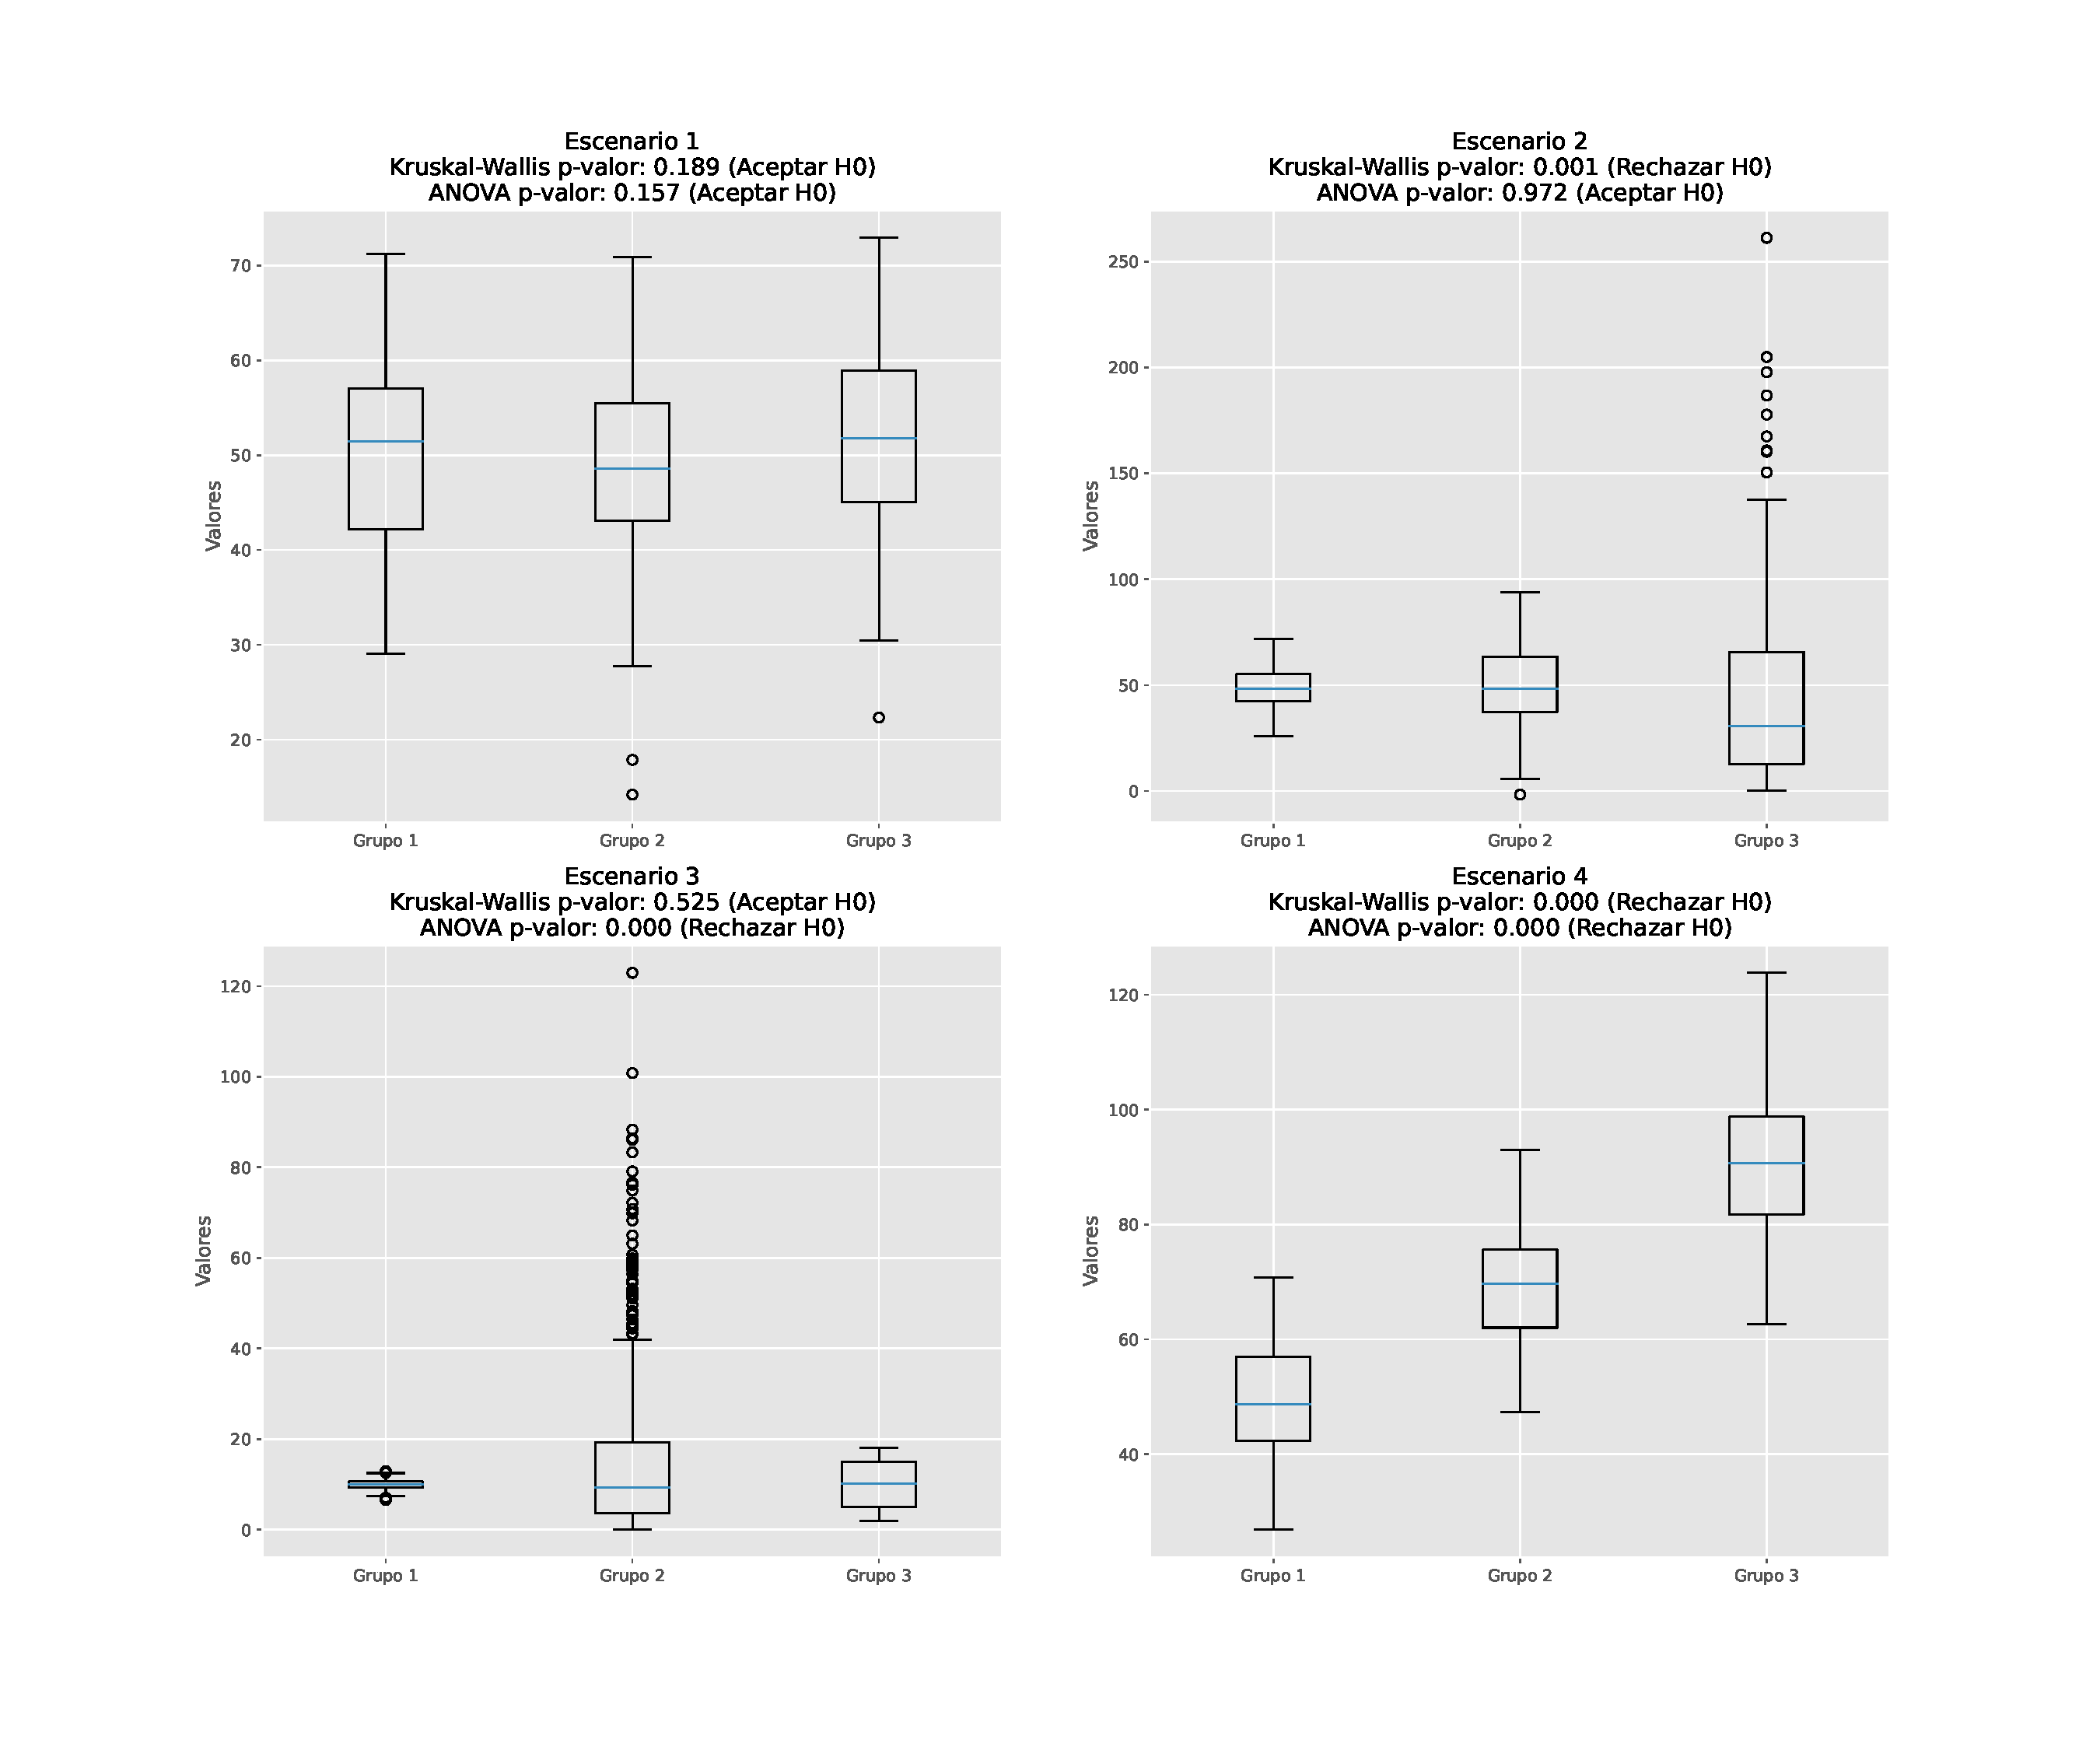
\includegraphics[width=\textwidth]{Figuras/kruskal.pdf}
%     \caption[Prueba de Kruskal]{Ilustración de la prueba de Kruskal.}
%     \label{fig:kruskal}
% \end{figure}


% En Kruskal-Wallis la hipótesis nula \( H_0 \) es que las medianas de todas las poblaciones son iguales mientras que la hipótesis alternativa \( H_1 \) es que al menos existe una de ellas donde la mediana es distinta. Las poblaciones no necesariamente tienen que tener el mismo número de elementos.

% Los supuestos de la prueba son los siguientes:
% \begin{itemize}
%     \item La variable de respuesta es ordinal o continua. Es decir existe una cantidad mejor a otra.
%     \item Independencia. Las observaciones de cada grupo son independientes entre sí.
%     \item Distribuciones tienen formas similares: Aunque no pedimos que sean normales, para comparar los rangos necesitamos que sean distribuciones similares con, tal vez, diferentes parámetros.
% \end{itemize} 

% Para construir el estadístico de prueba primero se hace un ranking de todos los elementos en todos los diferentes poblaciones, es decir, se ordenan todos los elementos de menor a mayor y se le asigna su posición en el ordenamiento a cada uno de ellos, a esta cantidad se le llama el rango del individuo $i$ \footnote{En este desarrollo se presenta la deducción para el caso donde no hay empates. }. 

% Después se calcula el rango promedio global, que se denota como \( \bar{R} \), mediante:

% $$
% \bar{R} = \frac{\sum_{i=1}^{g} R_i}{N} = \frac{1 + 2 + \ldots + N}{N} = \frac{N(N + 1)/2}{N} = \frac{N + 1}{2}.
% $$


% donde 
% \begin{itemize} 
%     \item \( g \) es el número de poblaciones o grupos.
%     \item \( n_i \) es el número de observaciones en la población \( i \).
%    \item \( N =\sum_{i=1}^n n_i\) es el número total de observaciones.
%    \item \( R_i =\sum_{j=1}^{n_i} R_{ij}\) es la suma de los rangos en la población $i$-ésima.
% \end{itemize}



% De la misma forma se define el rango promedio para cada población \(j\), \( \bar{R_j} \), se calcula como:

% $$
% \bar{R_j} = \frac{R_j}{n_j}.
% $$

% Ahora se calcula el cuadrado de la diferencia entre los rangos promedio con rango promedio global para cada población, ponderada por el tamaño de la misma, obteniendo:

% $$
% n_i (\bar{R_i} - \bar{R})^2 = n_i \left(\frac{R_i}{n_i} - \frac{N + 1}{2}\right)^2 = \frac{R_i^2}{n_i} - N (N+1) + \frac{n_i (N + 1)^2}{4}.
% $$

% Se suman todas estas diferencias para obtener:

% $$
% \sum_{i=1}^{g} \frac{R_i^2}{n_i} - g N (N + 1) + (N + 1)^2 \sum_{i=1}^{g} \frac{n_i}{4}.
% $$

% Así tenemos una cantidad que se comporta como una $\Xi$ cuadrada salvo un factor de normalización \( \frac{12}{N (N + 1)} \) para obtener \( H \) el estadístico de prueba:

% $$
% H = \frac{12}{N(N + 1)} \left(\sum_{i=1}^{g} \frac{R_i^2}{n_i} - N (N + 1)\right) + 3(N + 1).
% $$

% Y simplificando, se obtiene la Ecuación \ref{eq:Kruskal-Wallis} para $H$:

% \begin{equation} \label{eq:Kruskal-Wallis}
% H = \frac{12}{N(N + 1)} \sum_{i=1}^{g} \frac{R_i^2}{n_i} - 3(N + 1),
% \end{equation}

    
% La  \( H \) se distribuye como una distribución \( \chi^2 \) con \( g-1 \) grados de libertad. De esta forma podemos probar la hipótesis nula a una significancia de $\alpha$, rechazando si el $p$-valor es menor a $\alpha$ y aceptando si es mayor. 

% Podemos entender la Figura \ref{fig:kruskal} viendo que las distribuciones de los datos simulados se escogieron de modo que tuvieramos control sobre la media y la mediana de cada distribución. A ANOVA le importa la similitud entre las medias y a Kruskal-Wallis le importan los rangos. Entonces, al tomar una distribución con medias iguales y medianas diferentes obtenemos la subfigura superior derecha. Cambiando ahora la media, pero dejando la mediana igual (las lineas del boxplot están niveladas), tenemos que rechazamos ahora ANOVA (las medias son diferentes), pero aceptamos que las medianas son iguales y por lo tanto aceptamos $H_0$ para Kruskal-Wallis.

Ya teniendo el estadístico de prueba podemos comparar su probabilidad de ocurrencia bajo la hipótesis nula de acuerdo a un nivel de significancia prestablecido. 

\subsection{Prueba de Wilcoxon} \label{sec:Wilcoxon}

La prueba de Wilcoxon Signed-Rank \cite{Wilcoxon} es una prueba estadística no paramétrica que se utiliza para comparar dos muestras pareadas como vemos en la Figura \ref{fig:Wilcoxon}. Es una alternativa no paramétrica a la prueba $t$ de student \cite{geisserStatisticalPrinciplesExperimental1963} \textbf{para muestras pareadas} y es útil cuando no se pueden asumir distribuciones normales en la diferencia de las observaciones. 

\begin{figure}[H]
    \centering
    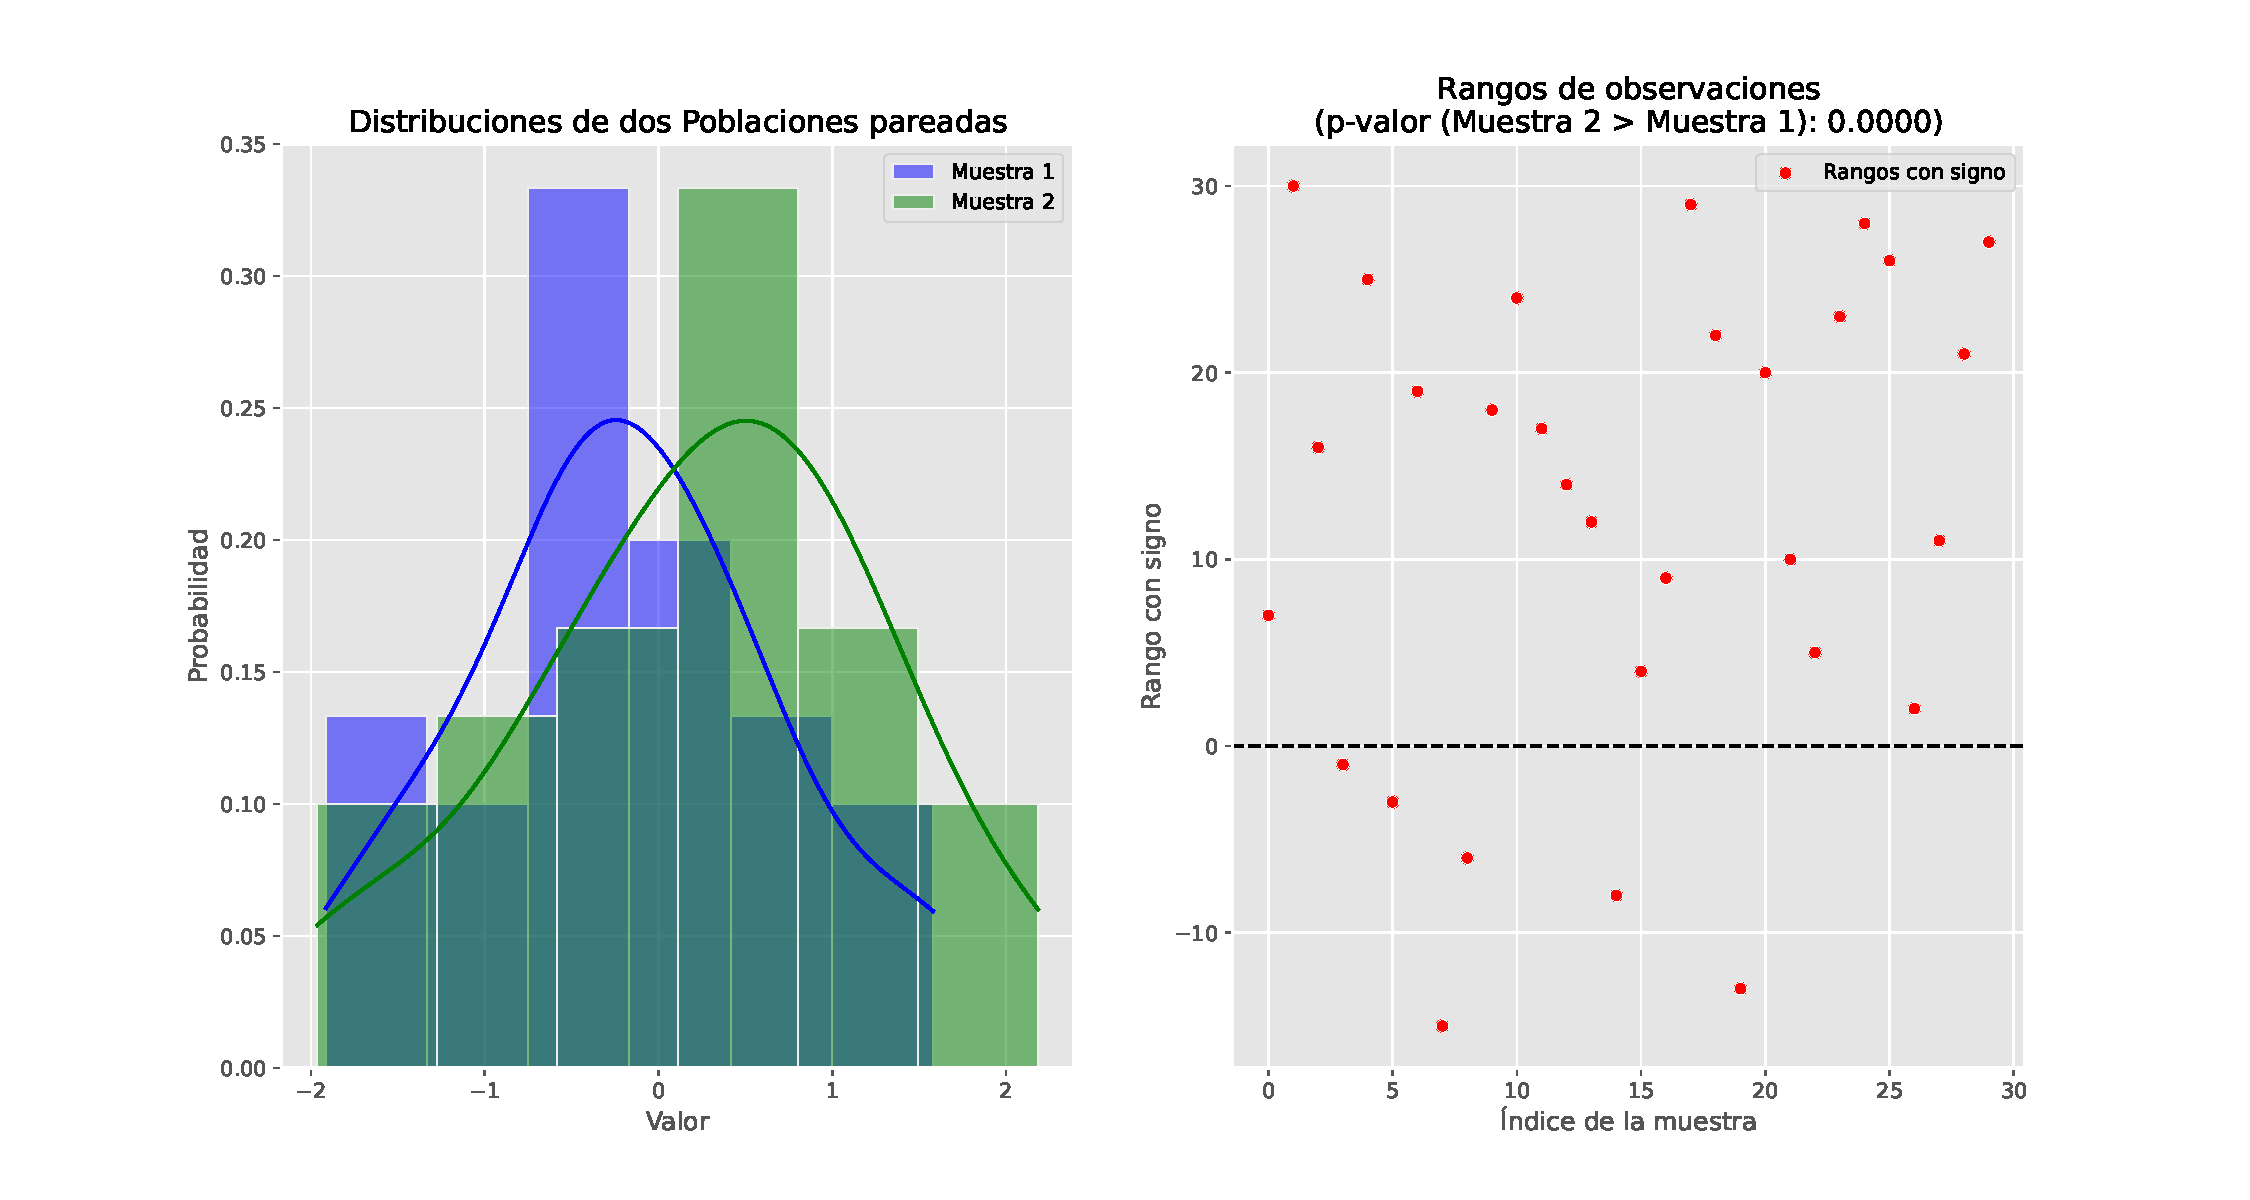
\includegraphics[width=\textwidth]{Figuras/Wilcoxon_vis.pdf}
    \caption{Visualización de lo que hace la prueba de Wilcoxon.}
    \label{fig:Wilcoxon}
\end{figure}


En el capítulo 4 realizaremos esta prueba para comparar algoritmos evolutivos multiobjetivo que tienen diferentes parámetros. Así, la discusión de esta prueba se da en términos de este caso particular.

Supongamos que tenemos un conjunto de $n$ entradas diferentes, que llamaremos poblaciones y denotaremos $P_i, i\in\{1,2,\ldots,n\}$. Estas poblaciones se inicializan de manera aleatoria, pero para cada $i$ se hace con una semilla diferente. Las poblaciones iniciales se mapean a un número real usando dos algoritmos distintos, $A_1,A_2$ \footnote{En nuestro caso las entradas son poblaciones de individuos que se evolucionan con ayuda de un EMOA. Los $A_1,A_2$ son el mismo algoritmo sólo que con diferentes hiperparámetros. Estos algoritmos tienen como salida una aproximación del frente de Pareto y el mapeo a los números reales $A_i(P_j)$ es un indicador de calidad que se obtiene de la aproximación al frente.} de modo que la salida del algoritmo son dos valores reales por cada población $A_1(P_i), A_2(P_i)$. Estos últimos resultados son dependientes porque comenzaron con la misma población, de modo que los consideramos observaciones pareadas. De este modo, obtenemos las diferencias de cada par de observaciones para obtener la Tabla \ref{tab:datos_pareados}.

\begin{table}[H]
    \centering
    \begin{tabular}{|c|c|c|c|}
    \textbf{Población Inicial $P_i$} & \textbf{Algoritmo 1} & \textbf{Algoritmo 2} & \textbf{Diferencias}    \\ \hline
    $P_1$                            & $A_1(P_1)$           & $A_2(P_1)$           & $Z_1=A_1(P_1)-A_2(P_1)$ \\
    $P_2$                            & $A_1(P_2)$           & $A_2(P_2)$           & $Z_2=A_1(P_2)-A_2(P_2)$ \\
    $\vdots$                         & $\vdots$             & $\vdots$             & $\vdots$                \\
    $P_n$                            & $A_1(P_n)$           & $A_2(P_n)$           & $Z_n=A_1(P_n)-A_2(P_n)$
    \end{tabular}
\caption[Algoritmos a comparar]{Vemos la estructura de los algoritmos a comparar.}
\label{tab:datos_pareados}
\end{table}


Las suposiciones de la prueba de Wilcoxon \cite{hollanderNonparametricStatisticalMethods2015} son parecidas a aquellas de la de Friedman:

\begin{itemize}
    \item Las observaciones pareadas tienen un carácter ordinal o real y los $Z_i$ son mutuamente independientes. 
    \item Cada $Z$ viene de una distribución continua que es simétrica alrededor de una mediana común $\theta$, llamada el efecto del tratamiento.
    %  Si $F_i$ es la función de probabilidad de $Z_i$, tenemos que 
    % $$ F_i(\theta+t)+F_i(\theta -t)=1, \,\, \forall t, i .$$
\end{itemize}

Ya con estas definiciones la hipótesis nula se puede formular como $$ H_0: \theta=0 $$
Es decir, cada una de las distribuciones (no necesariamente iguales entre cada $Z_i$)  de las diferencias entre un algoritmo y otro está distribuida simétricamente alrededor del 0. 

Para realizar la prueba hacemos lo siguiente 

\begin{itemize}
    \item Para cada par de observaciones pareadas \(i\), se calcula la diferencia \(d_i = x_i - y_i\).
    \item Se ordenan las diferencias absolutas \(|d_i|\) y se les asigna (al igual que en Friedman) rangos \(R_i\) desde el más pequeño al más grande. 
    \item Se separan las diferencias en dos grupos: diferencias positivas y diferencias negativas. Calculamos las sumas de los rangos para cada grupo  y las denotamos como \(W_+\) y \(W_-\) para las diferencias positivas y negativas respectivamente. Es decir, 
    \begin{align*}
    W_+= \sum_{d_i>0} \text{rank}(d_i) +\frac{1}{2}\sum_{d_i=0}\text{rank}(d_i), \nonumber\\
    W_-= \sum_{d_i<0} \text{rank}(d_i) +\frac{1}{2}\sum_{d_i=0}\text{rank}(d_i). \nonumber
    \end{align*}
\end{itemize}

El estadístico de prueba, está dado por el menor de \(W_+\) y \(W_-\), esto se debe a que estamos asumiendo que la distribución de las diferencias es la misma para cada una de ellas y es simétrica con respecto al origen ($\theta=0$). Entonces, la probabilidad de caer de un lado o del otro del cero sería de 1/2 y simplemente tenemos que ver cuál fue el número de casos que cayeron de un lado y ver la probabilidad de ocurrencia. Para dar un ejemplo concreto supongamos que tenemos $B$ casos donde la diferencia $Z$ es positiva. Después ordenamos estas diferencias para obtener los rangos\footnote{No hay menor o igual porque asumimos que las distribuciones son continuas, entonces la probabilidad de caer exactamente en el mismo punto es cero.} 

$$r_1 < r_2 <\cdots r_B.$$

Si tuvieramos, por ejemplo, 3 observaciones $Z_1,Z_2,Z_3$, la configuración de signos de estas observaciones nos da un total de 8 y bajo la $H_0$ cada uno de estos es igual de probable. Entonces tenemos $1/8$ de encontrar cada una de las configuraciones.

Lo que medimos con la prueba es la suma de rangos totales sí que supongamos que tenemos $T^+=3$, entonces basta contar las maneras de obtener este número para así obtener la probabilidad de que lo obtengamos dado que la hipotesis nula es cierta. De acuerdo a la Tabla \ref{tab:tmas}, tenemos que existen 2 formas de obtener $T^+=3$; cuando $r_1=3$ y cuando $r_1=1,r_2=2$, es decir, en el primer caso sólo existió una diferencia positiva $Z_i$ y fue la más pequeña de todas en valor absoluto, mientras que en el segundo hay dos diferencias positivas, las dos más grandes. Entonces vemos que la probabilidad de obtener $T^+=3$ esta dada por la suma de estos dos eventos y obtenemos $$ \mathbb{P}\left[ T^+=3 \right] =\frac{2}{8}.$$



\begin{table}[H]
    \centering
    \begin{tabular}{|c|c|c|c|}
    \textbf{B} & \textbf{$(r_1,\ldots,r_B)$} & \begin{tabular}[c]{@{}l@{}}Probabilidad de que\\ ocurra dado $H_0$\end{tabular} & $T^+=\sum_{i=1}^B r_i$ \\ \hline
    0          &                             & $\frac{1}{8}$                                  & 0                                                                                  \\
    1          & $r_1=1$                     & $\frac{1}{8}$                                  & 1                                                                                  \\
    1          & $r_1=2$                     & $\frac{1}{8}$                                  & 2                                                                                  \\
    1          & $r_1=3$                     & $\frac{1}{8}$                                  & 3                                                                                  \\
    2          & $r_1=1,r_2=2$               & $\frac{1}{8}$                                  & 3                                                                                  \\
    2          & $r_1=1, r_2=3$              & $\frac{1}{8}$                                  & 4                                                                                  \\
    2          & $r_1=2,r_2=3$               & $\frac{1}{8}$                                  & 5                                                                                  \\
    3          & $r_1=1,r_2=2,r_3=3$         & $\frac{1}{8}$                                  & 6                                                                                 
    \end{tabular}
\caption[Rankings y probabilidades]{Vemos todos los casos para los rankings de las diferencias positivas y su respectiva probabilidad.}
\label{tab:tmas}
\end{table}

Entonces se puede tomar como estadístico de prueba cualesquiera de las diferencias positivas y negativas y seguir el procedimiento de arriba. Para facilitar el cálculo de las combinaciones, se suele tomar el mínimo. Es decir, el estadístico para la prueba está dado por 

$$
T = \min(T_+, T_-).
$$


Para muestras grandes, la distribución de \(T\) se aproxima bien con una distribución normal y se puede convertir en una normal estándar con los siguientes factores

$$z= \frac{T-\frac{1}{4}N(N+1)}{\frac{1}{24}N(N+1)(2N+1)}.$$

Cuando se quiere hacer una prueba de un lado, es decir, si alguna de las poblaciones tiene mediana mayor o menor que otra, se toma solamente la parte positiva o negativa de las diferencias. Esto será útil en los siguientes capítulos cuando comparemos algoritmos ejecutados con diferentes configuraciones de parámetros. Una diferencia importante con respecto a la prueba $t$ es que, dado que la diferencia se convierte en rangos, no importa tanto la magnitud de la misma, sólo su orden relativo, de esta forma, la prueba de Wilcoxon no es tan sensible a outliers. 


\subsection{Análisis post-hoc y Family-wise Error Rate} \label{sec:FWER_Bonferroni}



En el análisis estadístico, cuando se realizan múltiples comparaciones o pruebas simultáneamente, incrementa la probabilidad de cometer errores de Tipo I (rechazar una hipótesis nula verdadera). Este fenómeno se conoce como la tasa de error familiar (FWER, por sus siglas en inglés: Family-wise Error Rate). La FWER es la probabilidad de cometer al menos un error de Tipo I entre todas las comparaciones.

Si se realizan $m$ pruebas estadísticas independientes, cada una con un nivel de significancia $\alpha$, la probabilidad de no cometer un error de Tipo I en una cada una de las prueba por sí misma es de $1 - \alpha$. Por lo tanto, la probabilidad de no cometer ningún error de Tipo I en las $m$ pruebas es $(1 - \alpha)^m$. Así, la probabilidad de cometer al menos un error de Tipo I es el complemento de este valor:

\begin{equation} \label{eq:FWER}
\text{FWER} = 1 - (1 - \alpha)^m.
\end{equation}

Al aumentar $m$, esta probabilidad crece, lo que incrementa el riesgo de falsas alarmas. Existen varios métodos para controlar la FWER, entre ellos se encuentra la corrección de Bonferroni.

La corrección de Bonferroni es una técnica que se considera conservadora y es usada  para ajustar los niveles de significancia y controlar el FWER. La idea básica es dividir el nivel de significancia $\alpha$ por el número total de pruebas $m$. Es decir, en lugar de utilizar $\alpha$ como el nivel de significancia para cada prueba individual, se utiliza $\alpha_{\text{Bonferroni}}$ definido como:

\begin{equation} \label{eq:Bonferroni}
\alpha_{\text{Bonferroni}} = \frac{\alpha}{m}.
\end{equation}

De esta manera, la probabilidad de cometer un error de Tipo I en cualquier prueba individual es reducida, y la probabilidad de cometer al menos un error de Tipo I en cualquiera de las $m$ pruebas se mantiene por debajo del nivel de significancia general $\alpha$.


\subsubsection{Limitaciones de las correcciones al FWER}

Es bastante debatido \cite{pernegerWhatWrongBonferroni1998}, \cite{nakagawaFarewellBonferroniProblems2004}, \cite{goemanMultipleHypothesisTesting2014}  cuando se debería de usar alguna corrección al FWER debido a que el error del que nos protege parece ser demasiado exigente. Las correcciones nos piden que ninguno de los rechazos de $H_0$ sea por probabilidad mayor a $\alpha$. Esto podría hacer que rechazáramos resultados interesantes sólo por el hecho de haber realizado análisis en conjunto. Esto quiere decir que puede llevar a un incremento en los errores de Tipo II (no rechazar una hipótesis nula falsa), reduciendo así el poder estadístico del análisis. Existen otras técnicas menos conservadoras, como la corrección de Holm-Bonferroni y la corrección de Sidak. De la misma forma de acuerdo a las dos pruebas expuestas anteriormente \ref{sec:Friedman}, \ref{sec:Wilcoxon}, se podría seguir un análisis tipo \textbf{post-hoc}. En este análisis, primero se realiza la prueba de Friedman y luego, con base en el resultado de la prueba, se realizarían las comparaciones uno a uno usando la prueba de Wilcoxon. Este análisis tendría los mismos problemas expuestos anteriormente.

Dadas las consideraciones expuestas en esta sección, en este trabajo presentaremos los resultados de las diferentes pruebas sin hacer alguna corrección, dejando este análisis a aplicaciones donde se requiera probar una hipótesis de manera específica.  



% \subsection{\textcolor{Azul}{Critical Difference Plots}}

% La prueba anterior se especificó para comparaciones uno a uno. Sin embargo, en este trabajo veremos comparaciones de muchos algoritmos (muchas combinaciones de hiperparámetros). Sería útil ver cómo realizar estas comparaciones y si es posible definir una prueba para establecer un orden parcial entre el desempeño de los algoritmos. Cuando comparamos uno a uno, podríamos concluir simplemente diciendo, por ejemplo: \emph{El algoritmo 1 superó al algoritmo 2, mientras que el 4 superó al 2 y al 3, pero no se encontraron otras diferencias significativas}. Sin embargo, como se nota en \cite{demsarStatisticalComparisonsClassifiers2006a}, por el sólo hecho de hacer muchas pruebas, una proporción de ellas rechazará $H_0$, este es el carácter aleatorio de las pruebas. Este problema es conocido en estadística y se suele atacar intentando controlar el error de familia, es decir, el error de hacer al menos un error de tipo I en las comparaciones múltiples. Entonces, primero se probaría la significancia de las diferencias entre muchas poblaciones con alguna prueba como ANOVA, Kruskal-Wallis o la prueba de Friedman. 

% Así, podemos hacer una prueba por partes en la que primero controlamos este error de familia. Y, sólo si la prueba rechaza su hipótesis nula (es decir, existen diferencias en la población), entonces proceder con la comparación uno a uno. Después, para visualizar cuáles grupos fueron significativamente diferentes de otros y tener una idea de cuál algoritmo fue mejor realizamos el siguiente procedimiento: 

% \begin{enumerate}
%     \item Realizamos la prueba para controlar el error de familia. Si esta prueba nos dice que hay diferencia entre poblaciones, seguimos.
%     \item Ordenamos acuerdo a cuál haya salido superior de acuerdo a alguna medida, como su media o mediana.
%     \item Calculamos el nivel de significancia de las pruebas uno a uno y unimos con líneas aquellos grupos que no son estadísticamente significativos.
% \end{enumerate}

% Este procedimiento nos da un Critical Difference plot \cite{demsarStatisticalComparisonsClassifiers2006a} como el de la Figura \ref{fig:CDP} donde vemos que se forman tres grupos entre los que no hay diferencia significativa, dados por $\{C4.5+m+cf,C4.5+m\,C4.5+cf\}, \{C4.5,C4.5+cf\} .$

% \begin{figure}[H]
%     \centering
%     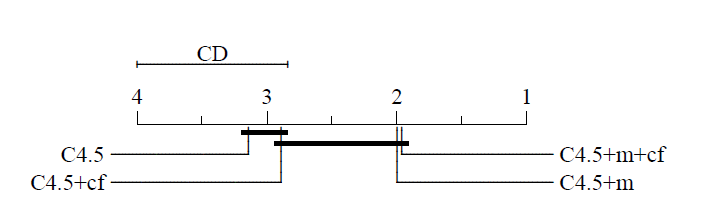
\includegraphics[width=\textwidth]{Figuras/cdp.png}
%     \caption[Critical Difference Plots]{Critical Difference Plot que compara cuatro clasificadores.}
%     \label{fig:CDP}
% \end{figure}



\subsubsection{Votación y conteo de borda} \label{sec:Votacion}

Si tenemos más de tres poblaciones a comparar, para decidir cuál de ellas tiene una mediana, por ejemplo, mayor, tendríamos que hacer comparaciones uno a uno de todos los pares poblacionales. Realizando seis pruebas de Wilcoxon en total. Después de esto, nos quedaríamos con un conjunto de \emph{victorias} de ciertas poblaciones sobre otras y, posiblemente, algunos resultados no significativos ¿Cómo escogeríamos a un ganador desde esta situación?

No siempre es el caso que podemos establecer sólo un orden parcial en el conjunto de votaciones. En particular, una elección que se puede tomar es el llamado \textbf{conteo de borda}. En este se cuentan \emph{victorias} totales que tiene una población sobre otra para determinar el ganador. Usaremos esta manera de indicar cuando un algoritmo tiene mejor desempeño que otro. De la misma forma que en la discusión de la Sección \ref{sec:FWER_Bonferroni}, un análisis que busque responder preguntas más específicas se puede derivar de los resultados de este trabajo. 








%%%%%%%%%%%%%%%%%%%%%%%%%%%%%%%%%%%%%%%%%%%%%%%%%%%%%%%%%%%%%%%%%%%%%%%%%
%                          Modelado                                     %
%%%%%%%%%%%%%%%%%%%%%%%%%%%%%%%%%%%%%%%%%%%%%%%%%%%%%%%%%%%%%%%%%%%%%%%%%
% \section{\textcolor{Azul}{Sección en color azul}}
% \subsection{SubSección}
% Antes de comenzar, se definen  en la Tabla ~\ref{tab:Tabla} los parámetros y variables utilizadas

% %%%%%%%%Tabla Nombres de parámetros
% \begin{table}[ht]                             %Inicia el entorno table debajo del texto
% \centering\                                     %   centra la Tabla
% \begin{tabular}{||c | c ||}                     %inicia entorno tabular con doble línea en las orillas, 2 columnas con el contenido centrado (c)
% \hline                                          %inserta línea horizontal
% \hline
% Nombre Parámetro/Variable & Símbolo\\
% \hline
% \hline
% Masa del péndulo & $m$ \\
% \hline
% Masa del carro & $M$\\
% \hline
% Distancia del eje de giro al centro de masa & $l$ \\
% \hline
% Aceleración gravitatoria & $g$ \\
% \hline
% Momento de inercia péndulo respecto del eje de giro& $J$ \\
% \hline
% Ángulo del péndulo respecto del eje vertical & $\theta$\\
% \hline
% Velocidad angular del péndulo & $\dot{\theta}$, $\omega$\\
% \hline
% Distancia del carro respecto al centro del riel & x\\
% \hline
% Velocidad del carro & $\dot{x}$, $v$\\
% \hline
% \hline
% \end{tabular}
% \caption[Parámetros dinámicos del carro-péndulo]{\textbf{Parámetros dinámicos del carro-péndulo} - Estos son los valores de parámetros utilizados en el diseño y las simulaciones, corresponden a los valores reales.}
% \label{tab:Tabla}                              %etiqueta para referencia
% \end{table}

% \blindtext


%%%%%%%%%%%%%%%%%%%%%%%%%%%%%%%%%%%%%%%%%%%%%%%%%%%%%%%%%%%%%%%%%%%%%%%%%
%                          SubSección
%%%%%%%%%%%%%%%%%%%%%%%%%%%%%%%%%%%%%%%%%%%%%%%%%%%%%%%%%%%%%%%%%%%%%%%%%

      % ~20 páginas - Explicar el problema en específico que se va a resolver, la metodología y experimentos/métodos utilizados

\chapter{Diseño Experimental}

En este capítulo se explica a detalle el procedimiento experimental que se usó para determinar si las combinaciones de diferentes pesos dan lugar a resultados significativamente diferentes bajo pruebas estadísticas.  Primero comenzamos recordando las características principales del algoritmo de PFI-EMOA y cuáles van a ser las modificaciones que haremos para explorar diferentes configuraciones de parámetros de la escalarización de Tchebycheff. Después, en la Sección \ref{sec:Proc_exp}, detallaremos el procedimiento experimental seguido para obtener los resultados. La siguiente parte del capítulo, la Sección \ref{sec:Marco_Exp}, detalla todos los valores usados en los diferentes experimentos realizados; es decir, cuántas combinaciones de pesos se usaron, cuántas corridas por algoritmo, en cuáles problemas, con cuántos objetivos, con cuántas variables de decisión, el número de evaluaciones de los algoritmos evolutivos, etc. Finalmente se concluye el capítulo en la Sección \ref{sec:Resultados}, detallando los resultados obtenidos así como algunas visualizaciones de agrupaciones de datos interesantes. En particular, se muestra el desempeño (conteo de borda) de cada combinación de pesos, conforme se aumenta el número de dimensiones y para cada indicador diferente. 


Como mencionamos anteriormente en la Sección \ref{sec:PFI-EMOA}, el algoritmo en el que estamos basándonos \cite{PFI} emplea non-dominated sorting para decidir qué solución eliminar, sin embargo, cuando no existe un candidato obvio (porque hay varios en el último nivel) se recurre al uso de indicadores de calidad. En este algoritmo se ocupan dos indicadores que, sólo por el hecho de medir cosas diferentes, van a tener objetivos conflictivos; estos dos indicadores son IGD+ (revisado en la Sección \ref{sec:IGDp}) y la Energía S de Riesz (revisada en la Sección \ref{sec:S-Energy}). 


\section{Procedimiento de experimentación con diferentes pesos} \label{sec:Proc_exp}

Como se mencionó en la Sección \ref{sec:PFI-EMOA}, el algoritmo PFI-EMOA \cite{PFI} realiza una escalarización constante de los dos indicadores de calidad (Energía S de Riesz e IGD+) para procurar que la solución no se estanque en convergencia ni tampoco en distribución. La forma de la escalarización está dada por la función aumentada de Tchebycheff dada en la Ecuación \ref{eq:tchebychev}.

\begin{equation} \label{eq:ATCH2}
    \text{ATCH}_{\vec{w}}=\max_{i=0,1} \{w_ix_i\}+\alpha (x_0+x_1),  
\end{equation}

donde $x_0$ sería el IGD+ y $x_1$ la energía S de Riesz en PFI-EMOA. Además los pesos son tales que $ w_0+w_1=1$ de modo que podemos entender la razón entre ambos como la importancia que le estamos dando a cada indicador y por lo tanto a cada objetivo de ese indicador. Por ejemplo, si $w_0=0.4$ y $w_1=0.6$ podríamos decir, a grandes rasgos, que estamos dando 60\% de importancia a promover la diversidad y 40\% a promover la convergencia.   

En \cite{PFI} se usaron diferentes escalarizaciones constantes para los problemas dependiendo del número de objetivos del problema a resolver. En particular, se usó $\vec{w}=(\frac{1}{2},\frac{1}{2})$ para MOPs de dos y tres objetivos, mientras que para mayor número de objetivos se usó $\vec{w}=(\frac{9}{10},\frac{1}{10})$. Esta decisión se realizó porque cuando se incrementa el número de objetivos, el número de soluciones no dominadas incrementa exponencialmente (como se discutió en la Sección \ref{sec:QIs}). En este caso la energía S de Riesz puede recompensar soluciones con poco grado de convergencia. Al incrementar la prioridad que se le da a IGD+ se debería incrementar la presión de selección. 

En este trabajo se extendió el análisis de \cite{PFI} utilizando diferentes combinaciones de pesos en \eqref{eq:ATCH} con el objetivo de explorar qué sucede cuando se le da un peso distinto a cada uno de los indicadores. Para comparar los resultados se usaron conjuntos de problemas prueba usados frecuentemente en el campo de optimización multiobjetivo debido a que presentan diferentes retos para que los algoritmos encuentren una buena aproximación al frente de Pareto. En particular se usaron 2 familias de problemas estándar en el campo de optimización multiobjetivo. Estos problemas prueba tienen las propiedad de ser escalables (se pueden definir para cualquier número de objetivos) y además presentan diferentes retos para encontrar buenas aproximaciones al frente de Pareto. El primer conjunto de problemas tiene el prefijo WFG (Walking Fishing Group) y fue presentada por primera vez en \cite{hubandScalableMultiobjectiveTest2005}. El segundo conjunto de problemas  tiene el prefijo de DTLZ y  fue presentada por primera vez en \cite{debScalableMultiobjectiveOptimization2002}. El desempeño de cada configuración de cada algoritmo se evalúa en cada problema prueba usando indicadores de calidad de la solución que arroja cada uno de ellos. Por ejemplo, para la combinación de $w_0=0.4$ y $w_1=0.6$ se deja correr el algoritmo hasta que se cumple su condición de paro y a la población resultante se le calculan uno de los indicadores de calidad presentes en la tabla \ref{Tabla:QIs}. Como cada uno de estos indicadores expresa una característica diferente de la solución, el tomador de decisiones tendría que escoger cuál de estas cantidades quisiera optimizar para tener una solución más cercana a sus preferencias. Nuestro objetivo es mostrar que existen diferencias para algunos de estos indicadores medidos sobre las poblaciones finales de los diferentes algoritmos (combinaciones de peso) de modo que podemos escoger una combinación específica de pesos si buscamos maximizar un indicador en particular.  
Así, para cada problema de prueba dado en la Tabla \ref{Tabla:problema_prueba}, se siguieron los pasos que se explican a continuación:

% TODO: Comenzar la discusión diciendo que se va a llamar algoritmos distintos a cada configuración de pesos.
% TODO: Poner el ejemplo desde el planteamiento de un problema y cómo se iría explorando la solución. 
\begin{enumerate}
    \item Se divide el espacio de pesos en 10 igualmente espaciados dados por 
    \begin{align} \label{eq:pesosw}
        \vec{w} \in \big\{ &(0.001,0.999),(0.1,0.9),(0.2,0.8),(0.3,0.7),(0.4,0.6) \nonumber\\
         &(0.5,0.5),(0.6,0.4),(0.7,0.3),(0.8,0.2),(0.9,0.1),(0.999,0.001) \big\}.
    \end{align}
    Siendo los primeros valores aquellos donde se toma más en cuenta el indicador de uniformidad (al ser menor $w_1$) y los últimos valores donde se prioriza el indicador de convergencia \footnote{Cabe destacar que los extremos de este conjunto $(0,1),(1,0)$ no se tomaron como tal porque daban lugar a los mismos resultados. Esto se discute en la siguiente sección.}.
    \item Para cada combinación de pesos en la Ecuación \ref{eq:pesosw}, se procede a ejecutar el algoritmo de PFI-EMOA, explicado en la Sección \ref{sec:PFI-EMOA}, con un número $f_{eval}=50,000$ de evaluaciones de la función de aptitud, es decir, $50000$  generaciones.
    \
    \item Cada una de las combinaciones de pesos se ejecuta un número $n_{runs}=10$ de veces con distintas configuraciones aleatorias de su población inicial. La inicialización está controlada por un conjunto de semillas fijas\footnote{El conjunto de semillas usadas se encuentra en el Apéndice \ref{sec:Apendice_semilla}.}, de esta forma se puede garantizar la reproducibilidad de los resultados.  

    \item Después, se procede al cálculo de los indicadores de calidad de cada población. Los indicadores que se trataron en este trabajo se pueden ver en la Tabla \ref{Tabla:QIs} que muestra cada uno de los indicadores junto su categoría principal de las revisadas en la Figura \ref{fig:carac_deseables_aprox}.
    \item Finalmente, después de realizar el cálculo de todos los indicadores de calidad, se realiza un análisis estadístico para determinar si tiene algún efecto el cambiar los pesos de la escalarización y, si lo tiene, cuál es el mejor y en qué medida. Esto se realiza por medio de las pruebas estadísticas de Kruskal-Wallis (para la parte de ver diferencias) y usando Wilcoxon como análisis post-hoc para ver cuáles de ellas son mejores a las otras.     
\end{enumerate}


\begin{table}[H]
    \centering
    \begin{tabular}{|c|c|}
    \textbf{Indicador} & \textbf{Categoría principal} \\ \hline
    \hyperref[sec:IGDp]{IGD+}      & Convergencia                  \\
    \hyperref[sec:R2]{R2}         & Convergencia                  \\
    \hyperref[sec:S-Energy]{Energía S}    & Diversidad                   \\
    \hyperref[sec:Epsilonp]{$\epsilon +$}       & Convergencia                  \\
    \hyperref[sec:IGD]{IGD}       & Convergencia                  \\
    \hyperref[sec:SPD]{SPD}        & Diversidad                   \\
    \hyperref[sec:HV]{Hipervolumen}        & Convergencia                 
    \end{tabular}
    \caption[QI para cada problema]{Indicadores de Calidad usados para cada uno de los problemas prueba. Para cada indicador se muestra la categoría principal en la que cae de las detalladas en la Sección \ref{sec:QIs_tax}. Cada indicador tiene un hipervínculo a la Sección que lo explica.}
    \label{Tabla:QIs}
\end{table}


A continuación se muestra la Tabla \ref{Tabla:problema_prueba} donde viene información relevante acerca de todos los problemas de prueba considerados, así como algunas características de su frente de Pareto. Cabe destacar que el número de variables de decisión está dado, como se menciona en \cite{PFI}, por $n=24+2(m-2)$, donde $m$ es el número de objetivos. Los problemas WFG también cuentan con parámetros relacionados a su posición, estos también están dados en términos del número de objetivos por $k=2(m-1)$. Para los problemas de la familia DTLZ, tenemos que el número de variables está dado por $n=m+l-1$, con $l=5$ para DTLZ1, $l=10$ para DTLZ2-DTLZ6 y $l=20$ para DTLZ7.

\begin{table}[H]
    \centering
    \resizebox{\textwidth}{!}{%
        \begin{tabular}{|l|l|l|l|l|l|l|}
        \textbf{Problema} & \textbf{Número de objetivos} & \textbf{Número de variables de decisión} & \textbf{Separabilidad}                                                           & \textbf{Frontalidad}                                                             & \textbf{Geometría}                                                         & \textbf{Sesgo}                                              \\ \hline
        DTLZ1             & 2,3,4,5,6,7                  & 6,7,8,9,10,11                            & separable                                                                        & multifrontal                                                                     & lineal                                                                     & no                                                          \\
        DTLZ2             & 2,3,4,5,6,7                  & 12,13,14,15,16                           & separable                                                                        & unifrontal                                                                       & cóncavo                                                                    & no                                                          \\
        \textbf{DTLZ3}    & 2,3,4,5,6,7                  & 12,13,14,15,16                           & separable                                                                        & multifrontal                                                                     & cóncavo                                                                    & no                                                          \\
        DTLZ4             & 2,3,4,5,6,7                  & 12,13,14,15,16                           & separable                                                                        & unifrontal                                                                       & cóncavo                                                                    & polinomial                                                  \\
        DTLZ5             & 2,3,4,5,6,7                  & 12,13,14,15,16                           & desconocido                                                                      & unifrontal                                                                       & degenerado                                                                 & dependiente de los parámetros                               \\
        DTLZ6             & 2,3,4,5,6,7                  & 12,13,14,15,16                           & desconocido                                                                      & unifrontal                                                                       & degenerado                                                                 & dependiente de los parámetros                               \\
        DTLZ7             & 2,3,4,5,6,7                  & 21,22,23,24,25,26                        & \begin{tabular}[c]{@{}l@{}}$f_{1:m-1}$ no aplica,\\ $f_m$ separable\end{tabular} & \begin{tabular}[c]{@{}l@{}}$f_{1:m-1}$ unimodal,\\ $f_m$ multimodal\end{tabular} & \begin{tabular}[c]{@{}l@{}}desconectado,\\ mixto\end{tabular}              & no                                                          \\
        WFG1              & 2,3,4,5,6,7                  & 24,26,28,30,32,34                        & separable                                                                        & unifrontal                                                                       & \begin{tabular}[c]{@{}l@{}}$f_{1:m-1}$ convexo,\\ $f_m$ mixto\end{tabular} & \begin{tabular}[c]{@{}l@{}}polinomial,\\ plano\end{tabular} \\
        WFG2              & 2,3,4,5,6,7                  & 24,26,28,30,32,34                        & no separable                                                                     & \begin{tabular}[c]{@{}l@{}}$f_{1:m-1}$ unimodal,\\ $f_m$ multimodal\end{tabular} & \begin{tabular}[c]{@{}l@{}}conexo,\\ desconectado\end{tabular}             & no                                                          \\
        WFG3              & 2,3,4,5,6,7                  & 24,26,28,30,32,34                        & no separable                                                                     & unifrontal                                                                       & \begin{tabular}[c]{@{}l@{}}lineal,\\ degenerado\end{tabular}               & no                                                          \\
        WFG4              & 2,3,4,5,6,7                  & 24,26,28,30,32,34                        & separable                                                                        & multifrontal                                                                     & cóncavo                                                                    & no                                                          \\
        WFG5              & 2,3,4,5,6,7                  & 24,26,28,30,32,34                        & separable                                                                        & deceptivo                                                                        & cóncavo                                                                    & no                                                          \\
        WFG6              & 2,3,4,5,6,7                  & 24,26,28,30,32,34                        & no separable                                                                     & unifrontal                                                                       & cóncavo                                                                    & no                                                          \\
        WFG7              & 2,3,4,5,6,7                  & 24,26,28,30,32,34                        & separable                                                                        & unifrontal                                                                       & cóncavo                                                                    & dependiente de los parámetros                               \\
        WFG8              & 2,3,4,5,6,7                  & 24,26,28,30,32,34                        & no separable                                                                     & unifrontal                                                                       & cóncavo                                                                    & dependiente de los parámetros                               \\
        WFG9              & 2,3,4,5,6,7                  & 24,26,28,30,32,34                        & no separable                                                                     & \begin{tabular}[c]{@{}l@{}}multifrontal,\\ deceptivo\end{tabular}                & cóncao                                                                     & dependiente de los parámetros                              
        \end{tabular}
    }
    \caption[Problemas prueba usados]{Problemas pruebas usados así como el total de variables objetivo $m$, de decisión,  y algunas características de su frente de Pareto.}
    \label{Tabla:problema_prueba}
    \end{table}

En estas dos últimas Tablas las características del frente de Pareto se refieren a lo siguiente:

\begin{itemize}
    \item \textbf{Separabilidad}: Un frente de Pareto es ``separable'' cuando las soluciones pueden clasificarse o separarse fácilmente en base a sus objetivos. Esto generalmente facilita la optimización, ya que puedes optimizar cada objetivo por separado y luego combinarlos.
    
    \item \textbf{Frontalidad}: Se refiere a la existencia de múltiples ``capas'' o ``frentes'' en el conjunto de soluciones no dominadas. En algunos casos, especialmente en problemas complejos, puede haber varias capas de soluciones que son no dominadas entre sí pero que son dominadas por soluciones en un frente superior.
    
    \item \textbf{Geometría}: Encontramos las siguientes categorías \begin{itemize}
        \item    Un frente de Pareto ``lineal'' sugiere que existe una relación lineal entre los objetivos en el frente óptimo. Esto puede simplificar mucho el problema de optimización, ya que las técnicas lineales son computacionalmente menos exigentes.
        
        \item \textbf{Cóncavo}: Un frente de Pareto ``cóncavo'' tiene una forma que se hunde hacia adentro, sugiriendo que hay una especie de ``compromiso'' entre los objetivos. En estos casos, mejorar en un objetivo puede llevar a un deterioro significativo en otro.
        
        \item \textbf{Degenerado}: Un frente ``degenerado'' contiene soluciones que son técnicamente no dominadas pero que son muy similares o idénticas en términos prácticos. Esto puede suceder debido a la discretización, errores numéricos o la naturaleza del problema de optimización. Por ejemplo que la dimensión del frente de Pareto no sea una menos que la del espacio de objetivos sino menor. 
        
        \item \textbf{Desconectado}: Un frente ``desconectado'' consiste en clústeres de soluciones no dominadas que están separadas entre sí. Esto podría implicar que hay ``saltos'' en el espacio de soluciones que son difíciles de cruzar mediante optimización continua.
        
        \item \textbf{Mixto}: Un frente ``mixto'' podría tener una combinación de varias de las características anteriores. Por ejemplo, podría ser en parte lineal y en parte cóncavo, o podría tener segmentos separables y no separables.
    \end{itemize}
    \item \textbf{Sesgo}: Que tanto se encuentra en la dirección de algún objetivo preferencialmente. 
\end{itemize}



\section{Marco Experimental} \label{sec:Marco_Exp}


Los parámetros de la Tabla \ref{Tabla:problema_prueba} nos ayudan a ejecutar el algoritmo con cada combinación de pesos. Sin embargo, los algoritmos evolutivos tienen un elemento aleatorio en cada una de sus etapas, como revisamos en la Sección \ref{sec:AE}, así que no podemos comparar simplemente la salida de una ejecución de dos algoritmos. Así, hacemos 10 ejecuciones de cada algoritmo, estas ejecuciones se realizan de modo que cada una de ellas tenga sus elementos aleatorios controlado por una semilla diferente; esto último nos garantiza reproducibilidad de los mismos resultados. 

Después de hacer las 10 ejecuciones para cada uno de los problemas con cada conjunto de pesos tenemos una población final por cada ejecución. De estas poblaciones nos interesa comparar su desempeño en los indicadores de la Tabla \ref{Tabla:QIs}. Entonces, para una combinación de pesos $\vec{w}_i$, de los valores disponibles en \eqref{eq:pesosw}, un problema prueba de los encontrados en la Tabla \ref{Tabla:problema_prueba}, con un número de objetivos específico, se ejecuta el algoritmo PFI-EMOA 10 veces con sus semillas respectivas. Así, se obtienen 10 conjuntos de soluciones como la que se observa en la Figura \ref{fig:aproximacion}. De estas 10 poblaciones se calcula cada valor de los indicadores de la Tabla \ref{Tabla:QIs} y entonces se obtiene un conjunto de valores de indicadores que se puede visualizar, por ejemplo, a través de un boxplot como el de la Figura \ref{fig:box}.

Los indicadores de calidad fueron calculados usando el programa de \emph{Assessment} utilizado en el Artículo \cite{PFI}. Al terminar de calcular todos los indicadores de calidad para todas las corridas para todos los problemas prueba en todas las dimensiones tenemos una tabla de valores de indicadores que tiene una cardinalidad dada por la Ecuación \ref{eq:cardinalidad}. 

\begin{align} \label{eq:cardinalidad}
    |\text{Valores de indicadores}|&=N_{ejec}*N_{indicadores}*N_{problemas}*N_{dimensiones}*N_{pesos} \nonumber\\
    &=10*7*16*6*11 \nonumber \\
    &=73920. 
\end{align}



\section{Resultados} \label{sec:Resultados}

En esta sección se muestran visualizaciones que se obtuvieron para cada problema y para cada indicador. Como el número de valores de indicadores es muy grande, como vimos en la Ecuación \ref{eq:cardinalidad}, se dejan las figuras completas en el Apéndice A.

Para cada problema y con el objetivo de poder detectar errores en el código y casos interesantes, se realizaron las siguientes visualizaciones:

\begin{itemize}
    % TODO: Poner primero una gráfica de la forma del DTLZ3 y luego de las aproximaciones
    \item Una función para visualizar la aproximación al frente de Pareto. Como podemos ver en las Figura \ref{fig:aproximacion} \footnote{Cuando el número de objetivos es mayor a 3 se usa una malla de proyecciones sobre cada uno de los objetivos} donde se grafica cada punto del conjunto de soluciones para el problema de DTLZ3 en 3 objetivos para todos los pesos, es decir, cada eje corresponde a un objetivo distinto . En 3 dimensiones, podemos visualizar la aproximación al frente de Pareto en todos los objetivos. En el caso de la Figura \ref{fig:aproximacion} vemos una malla de aproximaciones para los diferentes pesos. Comenzando en la esquina superior izquierda con $\vec{w}=(0.001,0.999)$ y continuando hacia la derecha hasta llegar al $\vec{w}=(0.999,0.001)$. Como podemos ver, casi todos tienen una configuración similar con la excepción de $\vec{w}=(0.1,0.9)$. Cabe destacar que esta malla fue generada con el algoritmo que usa como indicador de convergencia a IGD+.
    \item Además se produce una gráfica de coordenadas paralelas para ayudar a visualizar casos de mayores dimensiones como en la Figura \ref{fig:PCP}. Estas funciones se pueden tomar como una por cada ejecución, sin embargo para tomar una muestra que sea representativa del desempeño de cada configuración de algoritmos, tomamos aquella ejecución que está en la mediana del desempeño según el indicador de hipervolumen. Este tipo de visualizaciones son mucho más útiles cuando el número de objetivos es mayor a 3. Podemos ver cómo la misma combinación de la Figura \ref{fig:aproximacion} es la que se ve distinta por un outlier en la dirección $f_2$ que llega casi al valor de 2 del peso $w_0=0.1$. Al igual que en la imagen anterior, para esta visualización se usó el algoritmo que tiene a IGD+ como indicador de convergencia.
    \item Una función para visualizar un boxplot por cada problema y por cada indicador. Esto tiene un resumen de toda la información de cada una de las 10 ejecuciones para cada combinación de pesos, como en la Figura \ref{fig:box}.  Vemos en esa figura que hay variaciones entre los diferentes valores de $w_0$ aunque para tener algún tipo de confiabilidad tenemos que hacer las pruebas estadísticas de la siguiente sección. En esta figura se muestran los dos algoritmos, tanto con R2 como con IGD+ y podemos observar que a grandes rasgos se comportan similar, pero hay menor variación para R2. Esta observación la haremos más puntual más adelante.
    \item Una tabla con toda la información de cada valor del indicador.
\end{itemize}


\begin{figure} [H]
    \centering
    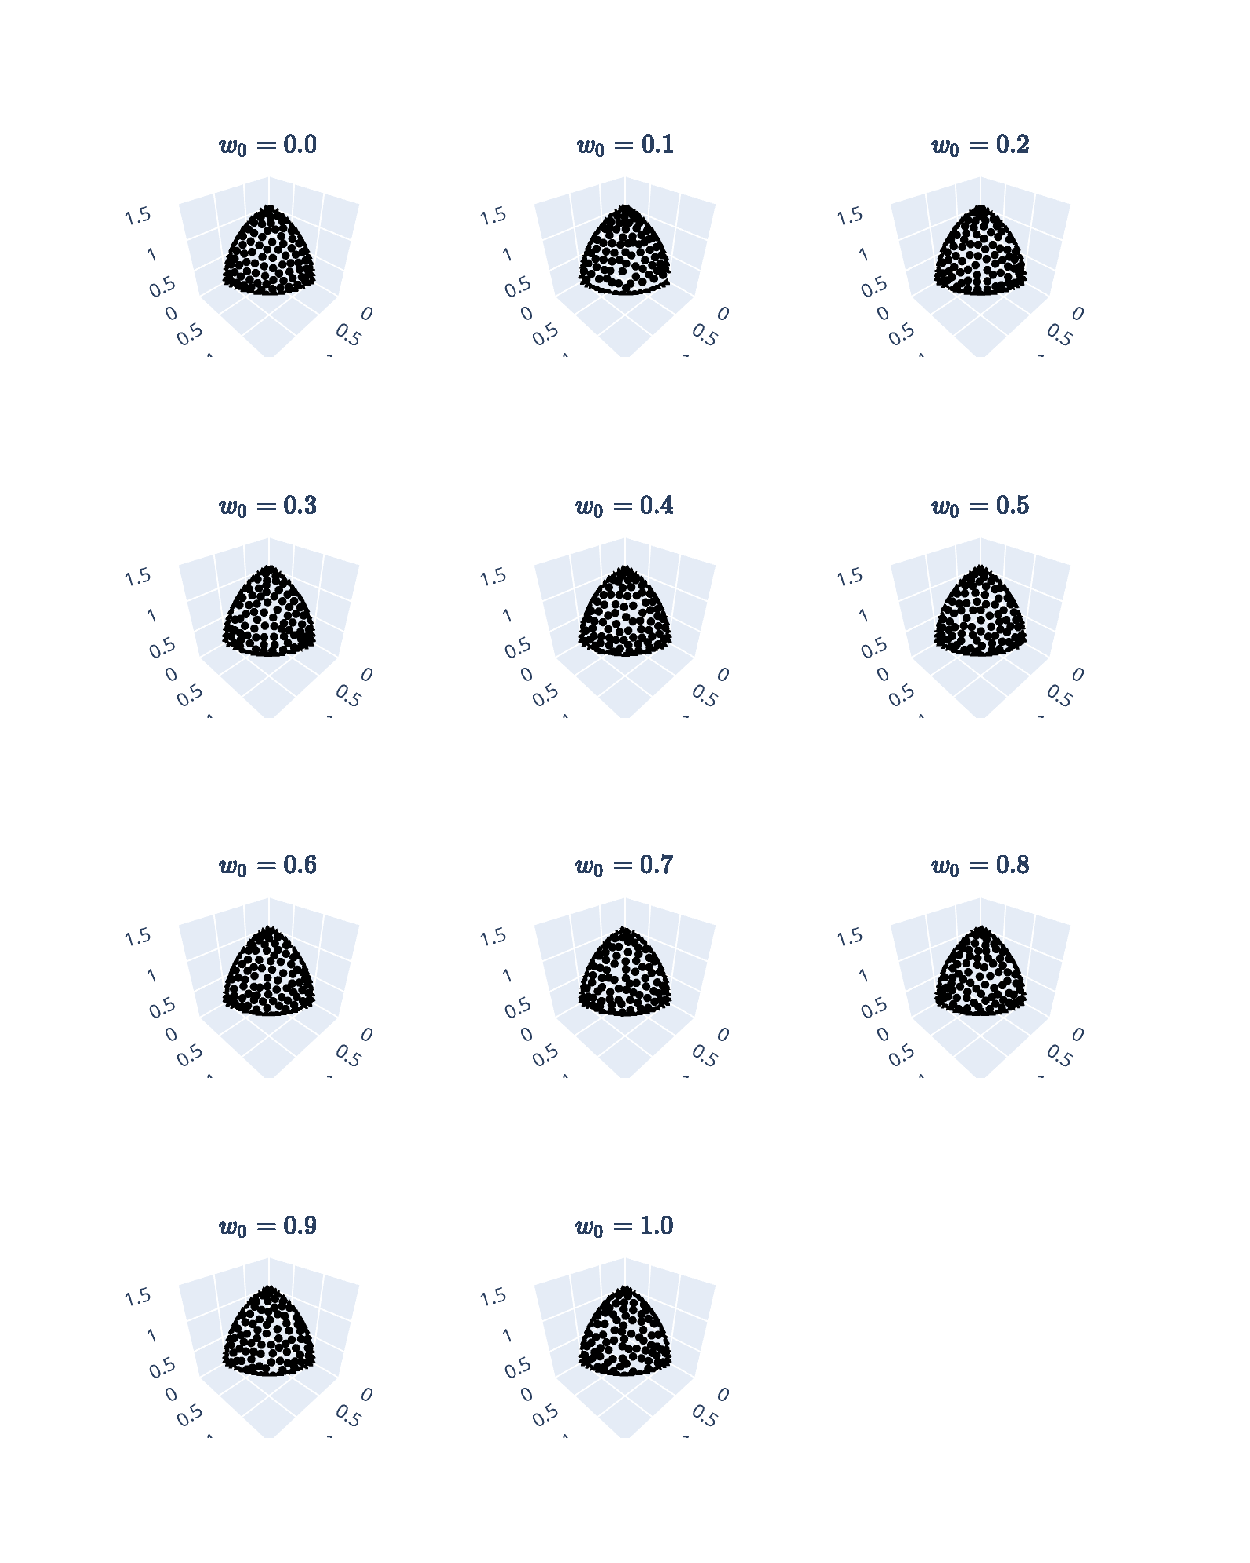
\includegraphics[width=\textwidth]{Figuras/DTLZ3_obj_3_alg_IGD+_indmed_HV_malla.pdf}
    \caption[Aproximación 3D al PF]{Malla de conjunto de aproximaciones para diferentes pesos para DTLZ3 en 3 objetivos.}
    \label{fig:aproximacion}
\end{figure}

\begin{figure} [H]
    \centering
    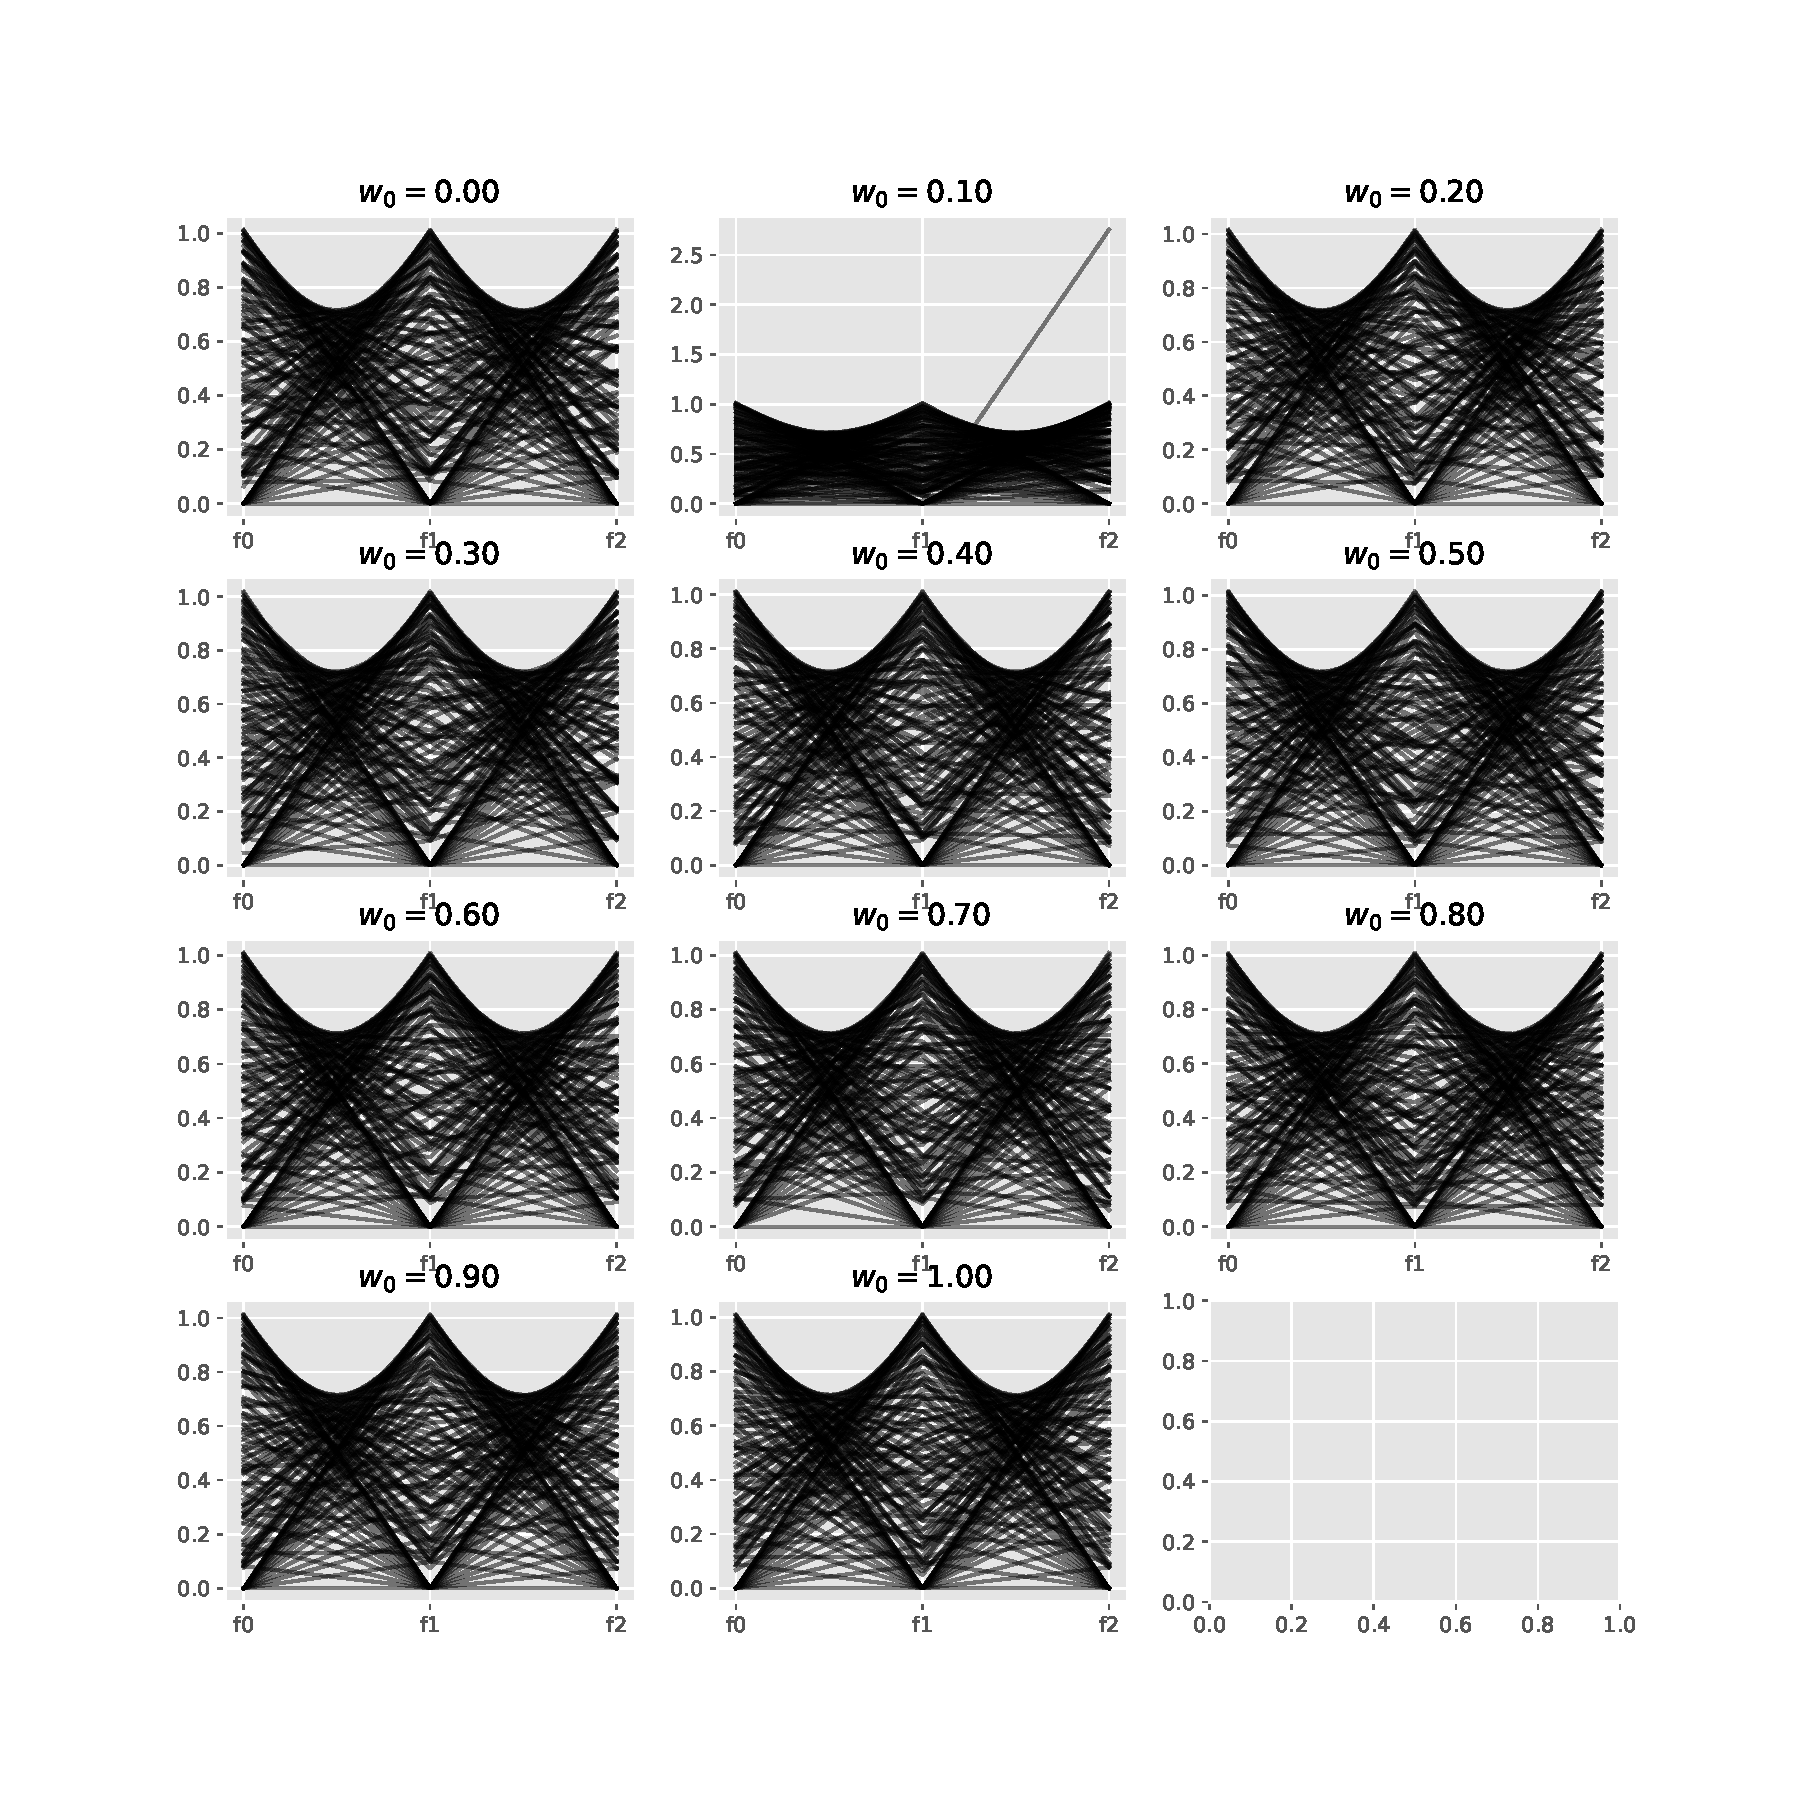
\includegraphics[width=\textwidth]{Figuras/DTLZ3_obj_3_alg_IGD+_indmed_HV_malla._PCP.pdf}
    \caption[Malla de PCP  de aproximaciones al PF.]{Malla de PCP para DTLZ3 en 3 objetivos.}
    \label{fig:PCP}
\end{figure}



\begin{figure} [H]
    \centering
    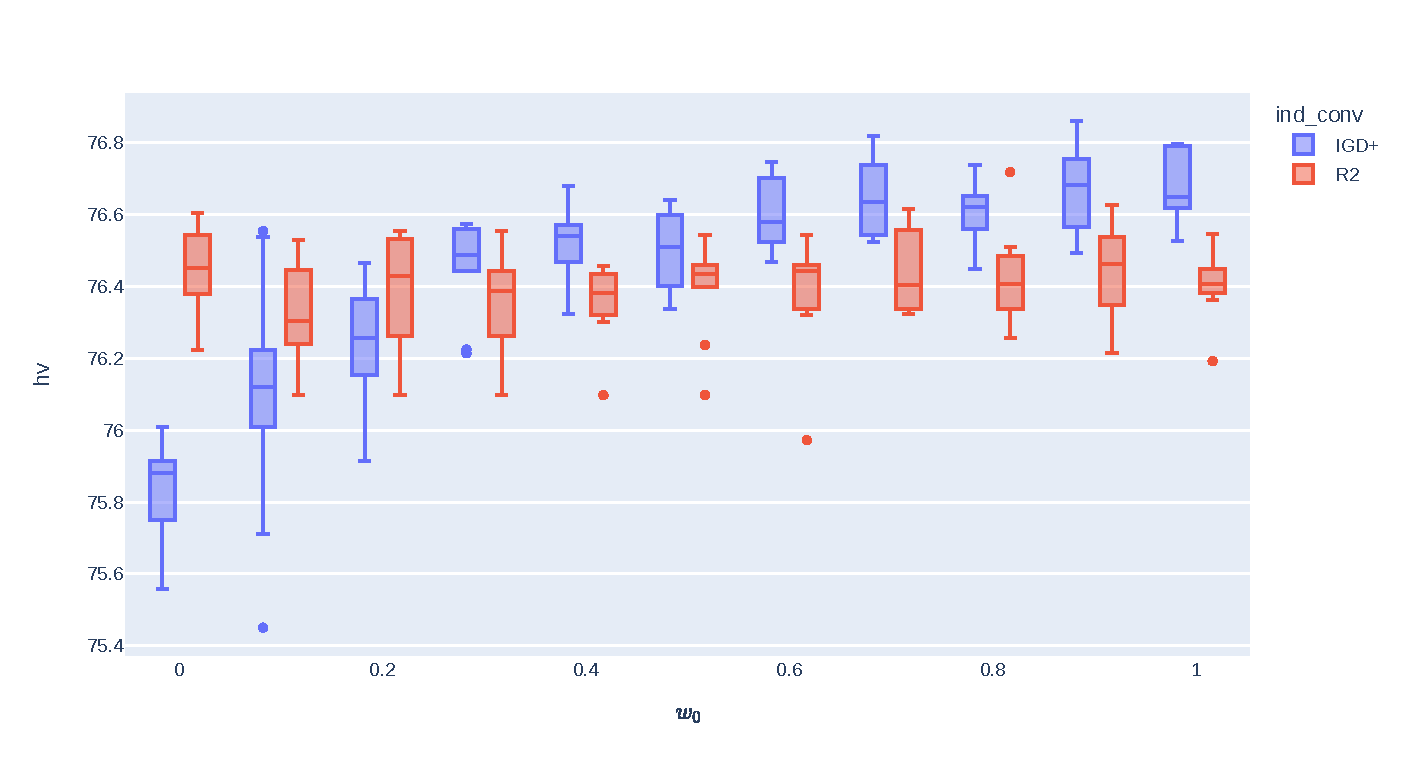
\includegraphics[width=\textwidth]{Figuras/WFG4_3obj_HV.pdf}
    \caption[Boxplot DTLZ3 HV.]{Boxplot DTLZ3 con 3 objetivos con el indicador de Hipervolumen. La variable ind\_conv indica qué indicador de calidad se usó en la combinación de Tchebycheff de la Ecuación \eqref{eq:tchebychev}.}
    \label{fig:box}
\end{figure}




\subsection{Pruebas Estadísticas}

Como se explicó en la Sección \ref{sec:pruebas_estadisticas}, para saber si un algoritmo tiene un desempeño diferente en un indicador dado usaremos la prueba de Kruskal-Wallis \ref{sec:Kruskal-Wallis}. Algunos resultados agregados de este procedimiento se pueden ver en las siguientes dos Figuras. En la primera imagen de la Figura \ref{fig:KW_dim_IGDp} se usó el algoritmo con IGD+ mientras que en la Figura \ref{fig:KW_dim_R2} R2. Podemos ver que en R2 existen mucho menos diferencias de acuerdo a Kruskal-Wallis.   La prueba sólo indica si hay una diferencia significativa entre al menos una de las observaciones con el resto. Vemos que importa mucho ajustar los pesos para indicadores como IGD+, HV, IGD y en menor medida para S-energy. Vemos que para dos dimensiones parece importar menos que pesos escojamos para el desempeño de todos los indicadores.

\begin{figure}[H]
    \centering
    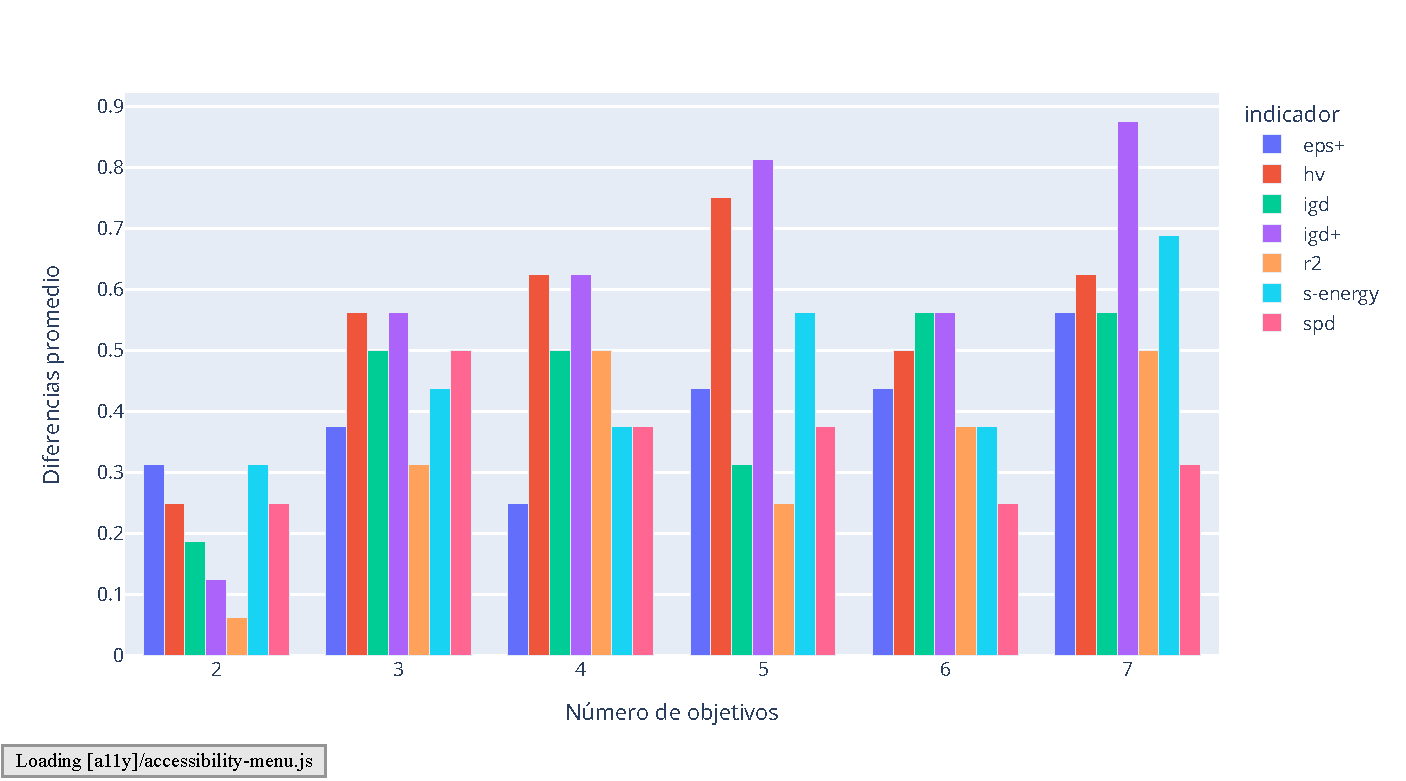
\includegraphics[width=\textwidth]{Figuras/KW_obj_indconv_IGD+.pdf}
    \caption[Kruskal-Wallis IGD+]{Diferencias cuando el indicador de convergencia de ATCH es IGD+.}
    \label{fig:KW_dim_IGDp}
\end{figure}

\begin{figure}[H]
    \centering
    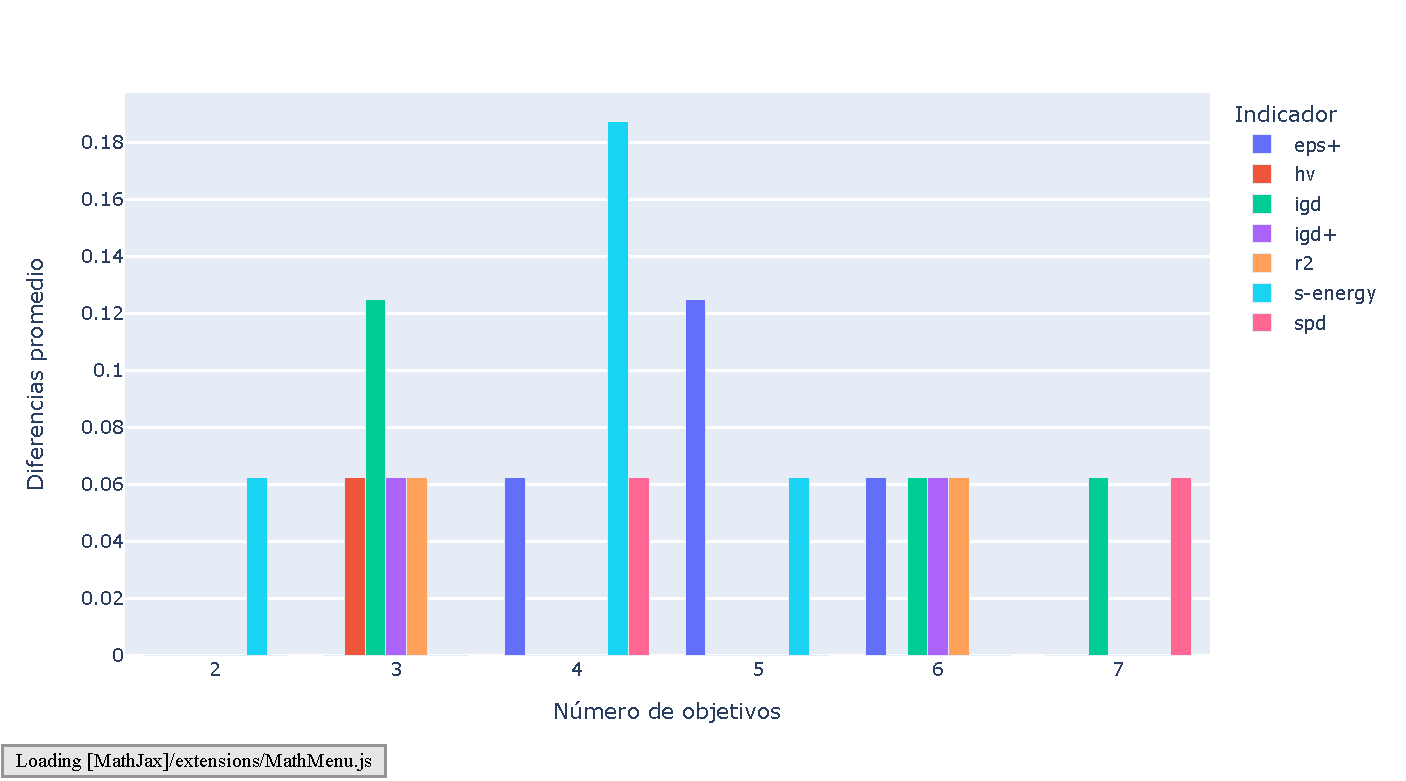
\includegraphics[width=\textwidth]{Figuras/KW_obj_indconv_R2.pdf}
    \caption[Kruskal-Wallis R2]{Diferencias cuando el indicador de convergencia de ATCH es R2.}
    \label{fig:KW_dim_R2}
\end{figure}


De la misma forma, en la Figura \ref{fig:KW_conv_dist_IGDp} hacemos una agregación por categoría de Indicador para el caso donde el indicador de convergencia en el estimador de densidad es IGD+, mientras que para R2 tenemos la Figura \ref{fig:KW_conv_dist_R2}. Nuevamente observamos como el algoritmo de IGD+ presenta más sensibilidad a la elección de parámetros. Basándonos en la clasificación de la Tabla \ref{Tabla:QIs} separamos los problemas para ver si se va volviendo más importante la selección de $w_0$ conforme aumentamos la dimensión. Vemos que el número de objetivos parece importar un poco más para los indicadores convergencia y obtenemos el mismo resultado de la figura anterior, en el sentido en el que para 2 objetivos no parece importar mucho la escalarización que usemos.

\begin{figure}[H]
    \centering
    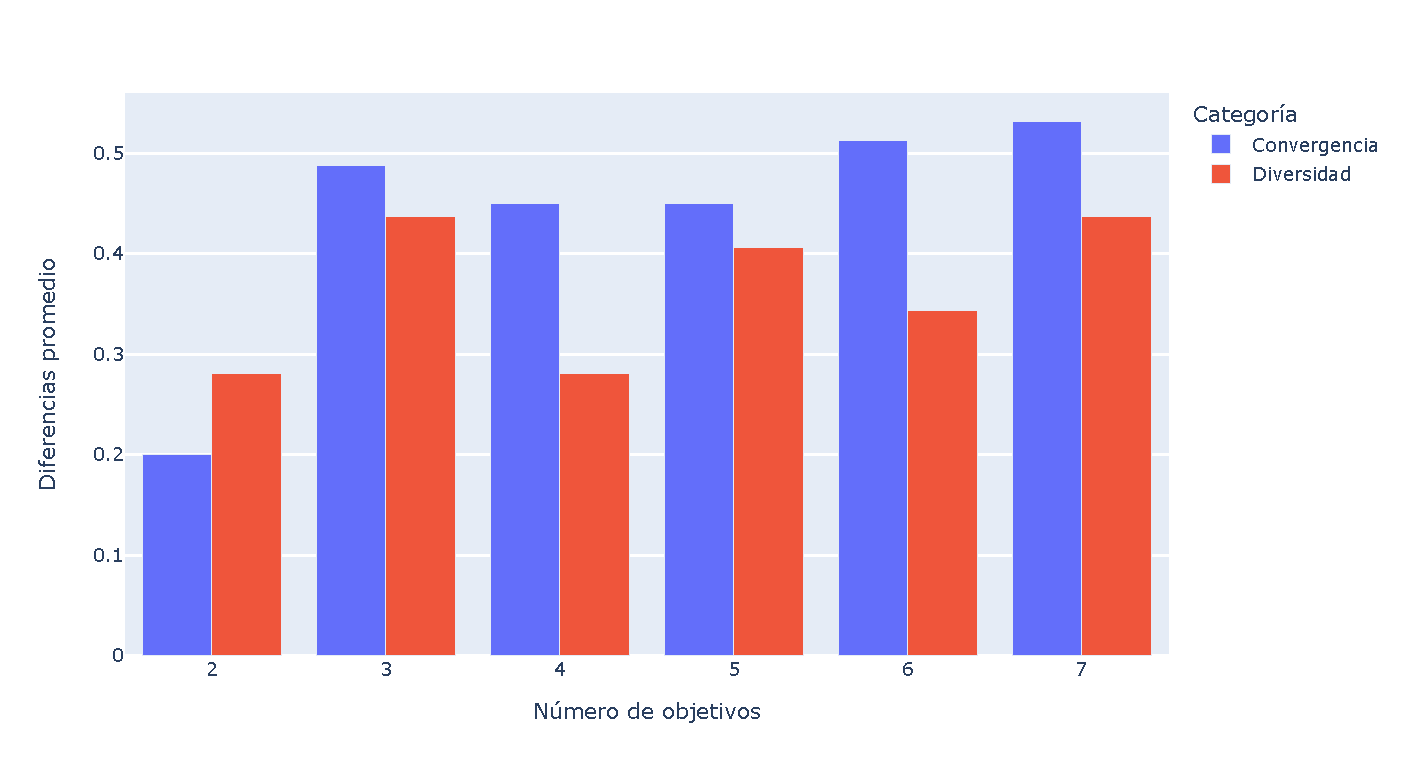
\includegraphics[width=\textwidth]{Figuras/KW_Diferencia_por_categoria_IGD+.pdf}
    \caption[Kruskal-Wallis por categoría para IGD+.]{Kruskal-Wallis por categoría de indicadores de acuerdo a la Tabla \ref{Tabla:QIs} cuando el indicador de convergencia de ATCH es IGD+.}
    \label{fig:KW_conv_dist_IGDp}
\end{figure}

\begin{figure}[H]
    \centering
    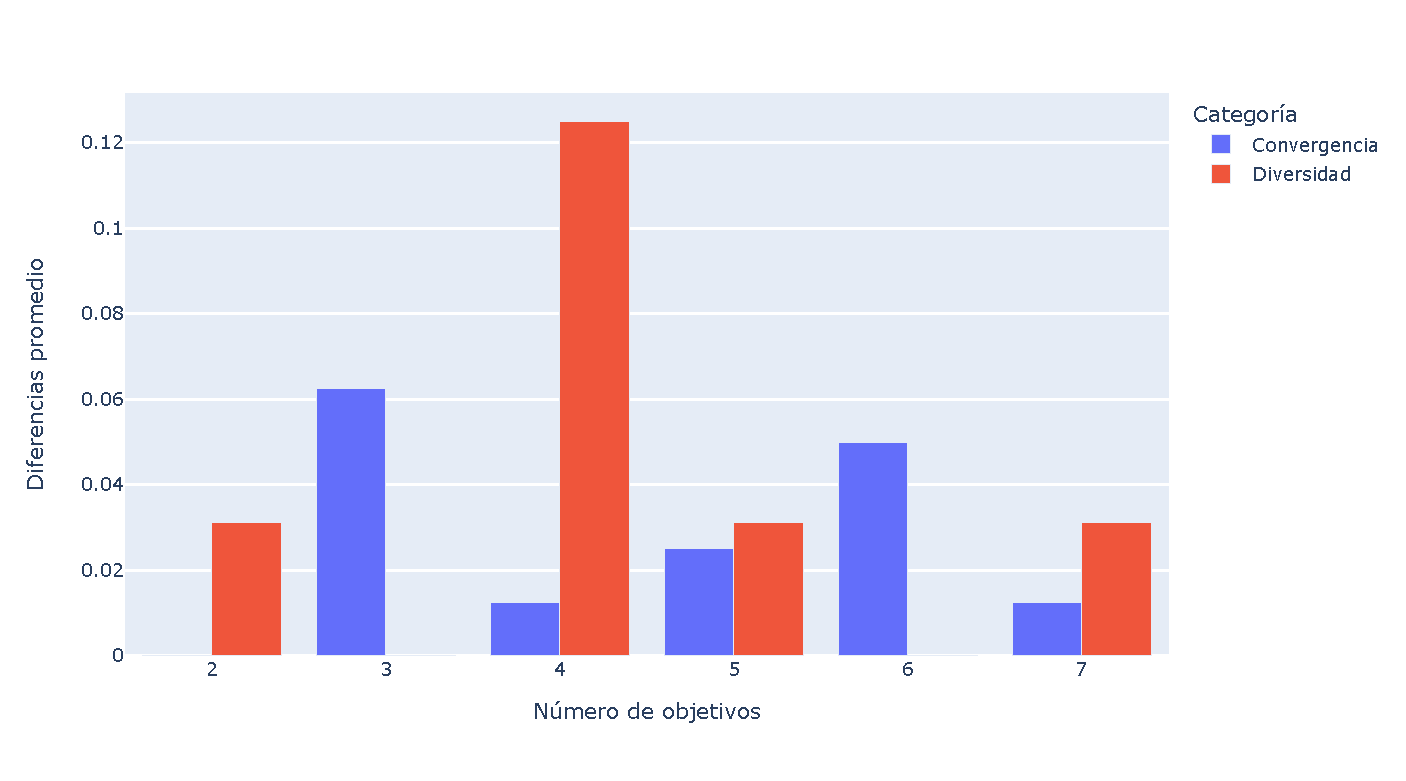
\includegraphics[width=\textwidth]{Figuras/KW_Diferencia_por_categoria_R2.pdf}
    \caption[Kruskal-Wallis por categoría para R2.]{Kruskal-Wallis por categoría de que indicador usamos de acuerdo a la Tabla \ref{Tabla:QIs} cuando el indicador de convergencia de ATCH es R2.}
    \label{fig:KW_conv_dist_R2}
\end{figure}


\section*{Comparación uno a uno}
Para saber si un algoritmo $A_1$ tiene un mejor desempeño que otro algoritmo $A_2$ usaremos la prueba de Wilcoxon que revisamos en la Sección \ref{sec:Wilcoxon}. Así, comparando con los diferentes valores de los pesos para la escalarización, obtenemos una Tabla como la de la Figura \ref{fig:heat}. En esta figura la hipótesis nula es que el peso del renglón no es mejor que el de la columna. Hay que recordar que algunos indicadores son maximizados y otros minimizados así que hay que escoger la dirección correcta en la implementación de scipy.stats. Es de esperarse que los valores altos de $w_0$ den como resultado un mejor hipervolumen pues es para estos que se favorece el indicador de convergencia.

\begin{figure} [H]
    \centering
    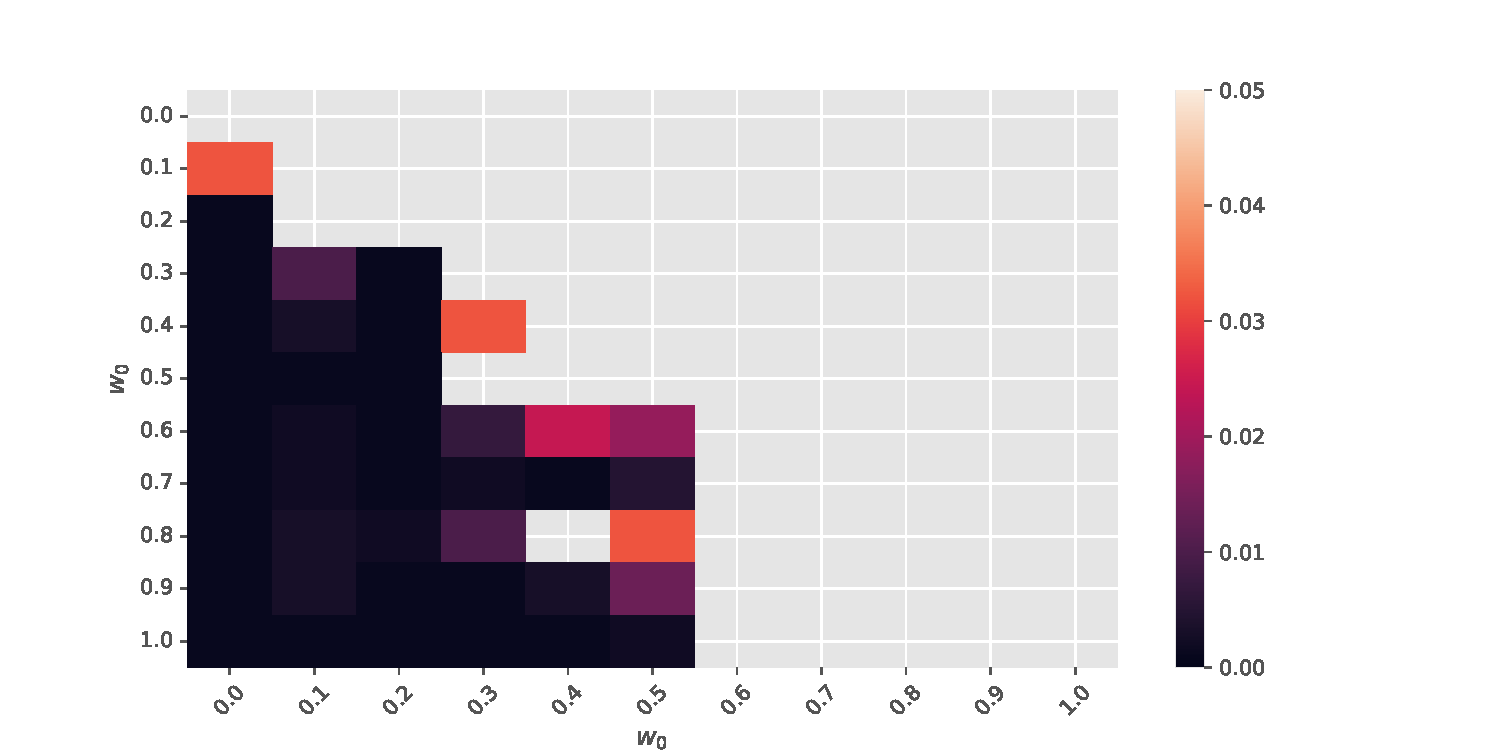
\includegraphics[width=0.8\textwidth]{Figuras/Heatmap_WFG4_obj3_hv_indconv_IGD+.pdf}
    \caption[Heatmap Wilcoxon]{Vemos un mapa de calor con el valor de la prueba $p$ para la prueba de Wilcoxon. }
    \label{fig:heat}
\end{figure}

Podemos obtener el número de las victorias de cada uno de los valores si simplemente contamos cuántas pruebas resultan ser significativamente mejores. Es decir, contando cuántos cuadros hay en la Figura en \ref{fig:heat} están coloreados para una columna dada. A esta manera de establecer ganadores se le conoce como conteo de borda y lo podemos visualizar en la Figura \ref{fig:borda_problema}.

\begin{figure}[H]
    \centering
    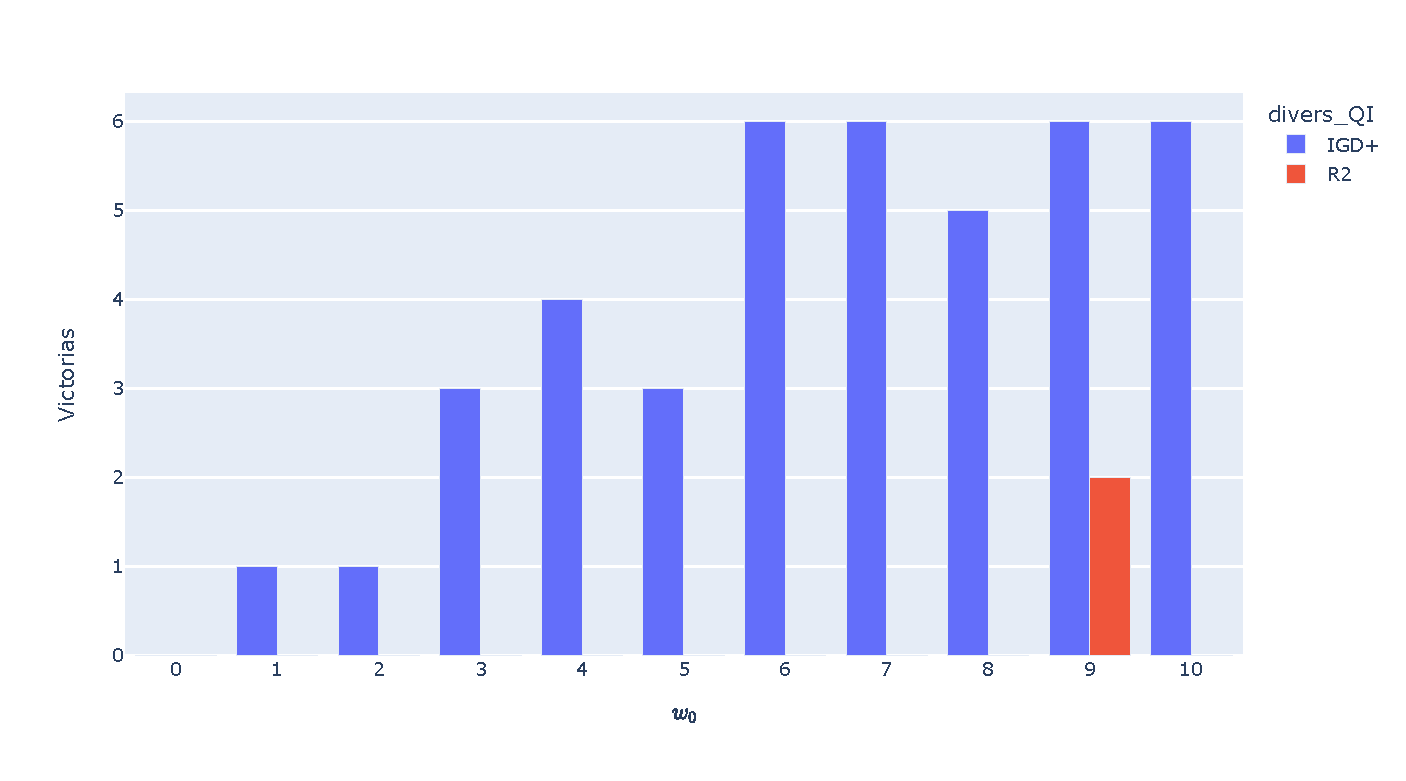
\includegraphics[width=\textwidth]{Figuras/conteo_borda_WFG4_obj3_indhv.pdf}
    \caption[Conteo de borda]{Conteo de borda de cada peso. Es útil comparar esta Figura con \ref{fig:heat}.}
    \label{fig:borda_problema}
\end{figure}

Vemos de la Figura \ref{fig:borda_problema} que a mayor peso suele haber más victorias, sin embargo, el valor de 0.7 parece haber encontrado un caso interesante en el que un mayor énfasis en la energía S ayuda a mejorar las victorias en un indicador de convergencia como el Hipervolumen. 

\subsection{Agregación por número de objetivos}

En esta sección se realizan agregaciones por número de objetivos de todos los conteos de borda. Es decir, estamos uniendo todos los indicadores sin importar si son de convergencia o distribución. Las siguientes Figuras\ref{fig:borda_obj_2}, \ref{fig:borda_obj_3}, \ref{fig:borda_obj_4}, \ref{fig:borda_obj_5}, \ref{fig:borda_obj_6} y  \ref{fig:borda_obj_7} nos muestran el número de victorias promedio para cada peso. Esto es, de todos los problemas considerados para cada número de objetivos, cuánto sale el conteo de borda de un valor fijo de $w_0$. Es decir, cuántas victorias tiene con respecto a todos los otros pesos.   

\begin{figure} [H]
    \centering
    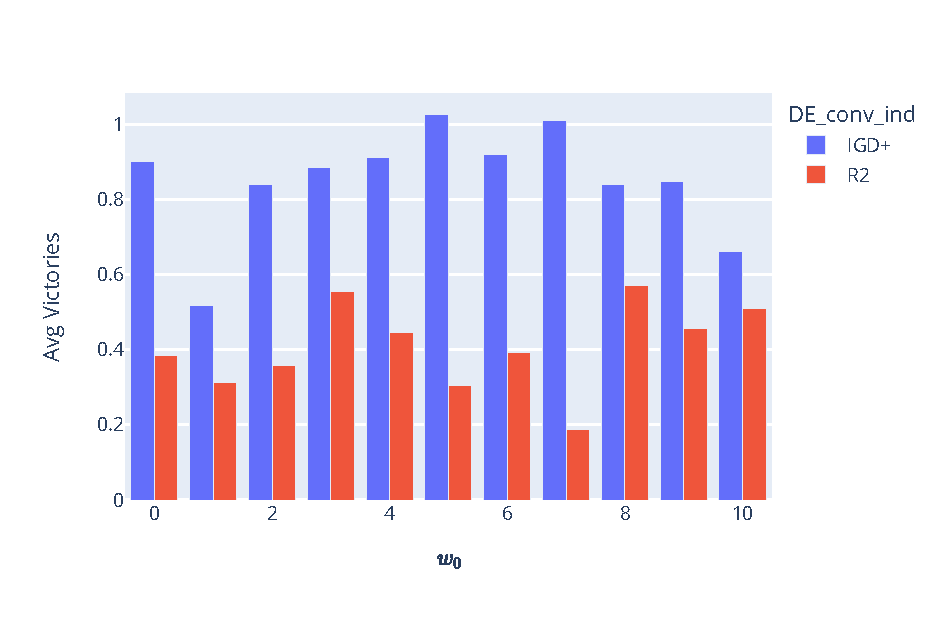
\includegraphics[width=\textwidth]{Figuras/borda_obj_2.pdf}
    \caption[Conteo de borda por número de objetivos]{Quién gana más, para todos los indicadores, conforme cambiamos el peso, para 2 objetivos.}
    \label{fig:borda_obj_2}
\end{figure}

\begin{figure} [H]
    \centering
    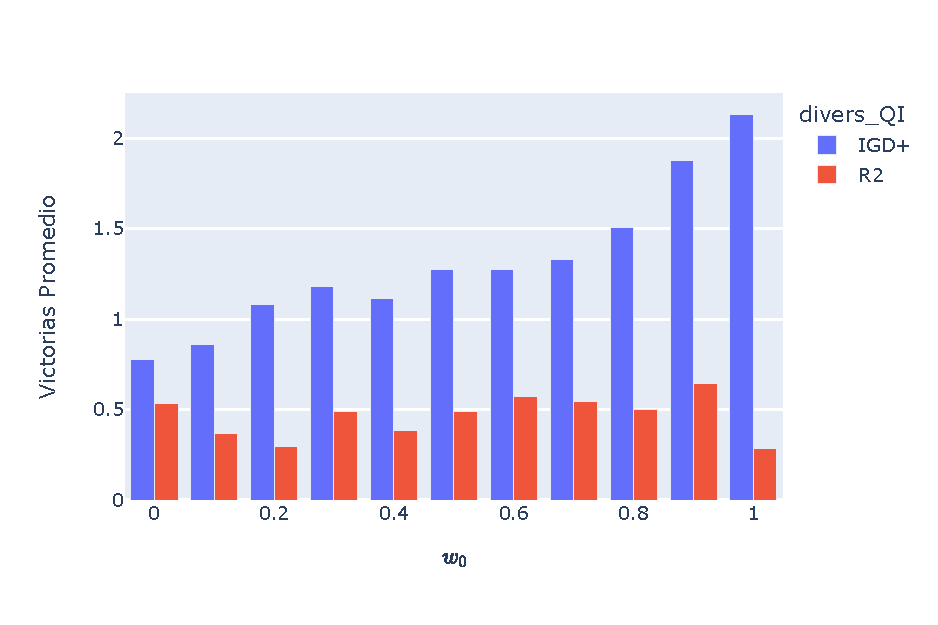
\includegraphics[width=\textwidth]{Figuras/borda_obj_3.pdf}
    \caption[Conteo de borda por número de objetivos]{Quién gana más, para todos los indicadores, conforme cambiamos el peso, para 3 objetivos.}
    \label{fig:borda_obj_3}
\end{figure}

\begin{figure} [H]
    \centering
    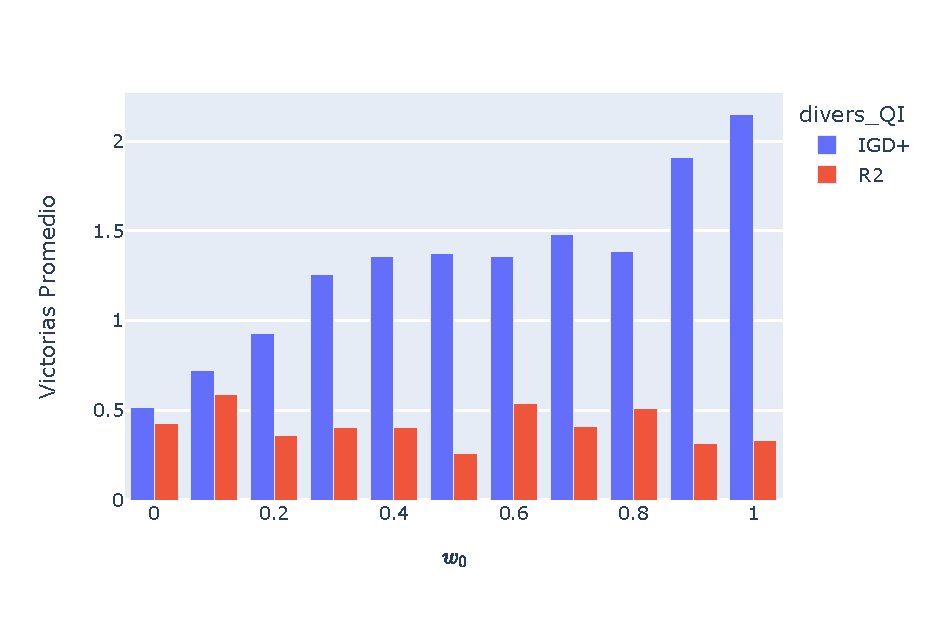
\includegraphics[width=\textwidth]{Figuras/borda_obj_4.pdf}
    \caption[Conteo de borda por número de objetivos]{Quién gana más, para todos los indicadores, conforme cambiamos el peso, para 4 objetivos.}
    \label{fig:borda_obj_4}
\end{figure}

\begin{figure} [H]
    \centering
    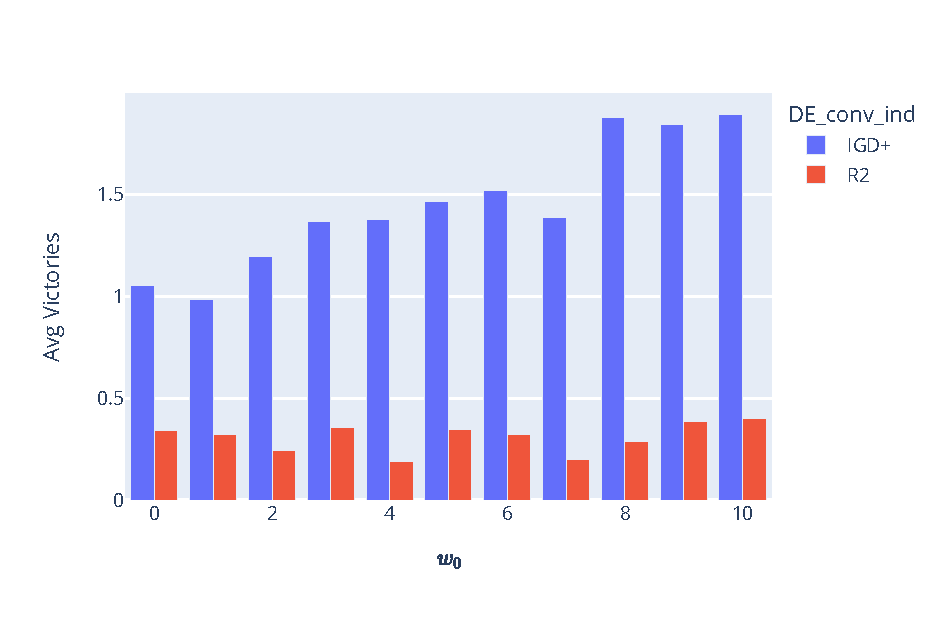
\includegraphics[width=\textwidth]{Figuras/borda_obj_5.pdf}
    \caption[Conteo de borda por número de objetivos]{Quién gana más, para todos los indicadores, conforme cambiamos el peso, para 5 objetivos.}
    \label{fig:borda_obj_5}
\end{figure}

\begin{figure} [H]
    \centering
    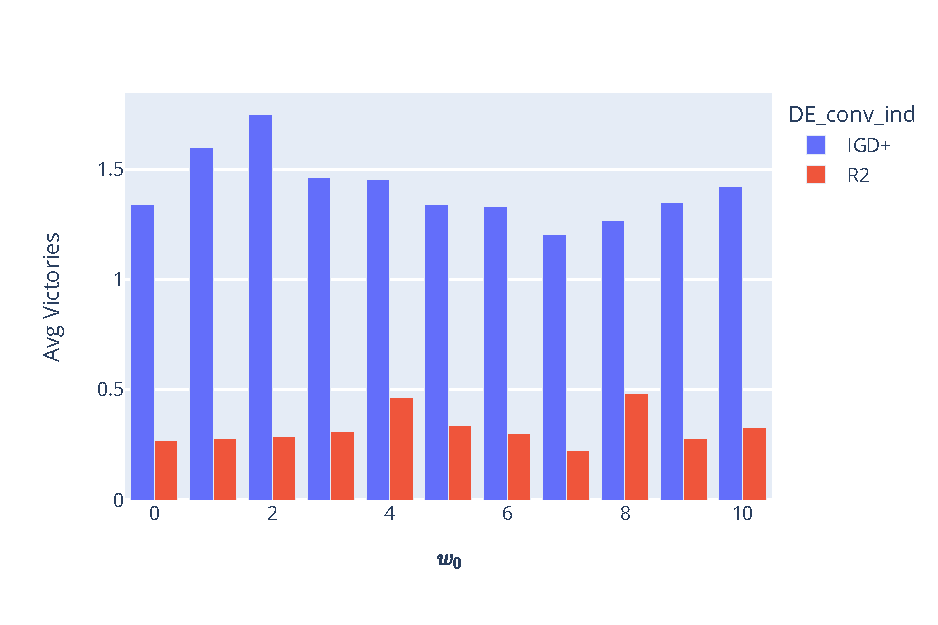
\includegraphics[width=\textwidth]{Figuras/borda_obj_6.pdf}
    \caption[Conteo de borda por número de objetivos]{Quién gana más, para todos los indicadores, conforme cambiamos el peso, para 6 objetivos.}
    \label{fig:borda_obj_6}
\end{figure}

\begin{figure} [H]
    \centering
    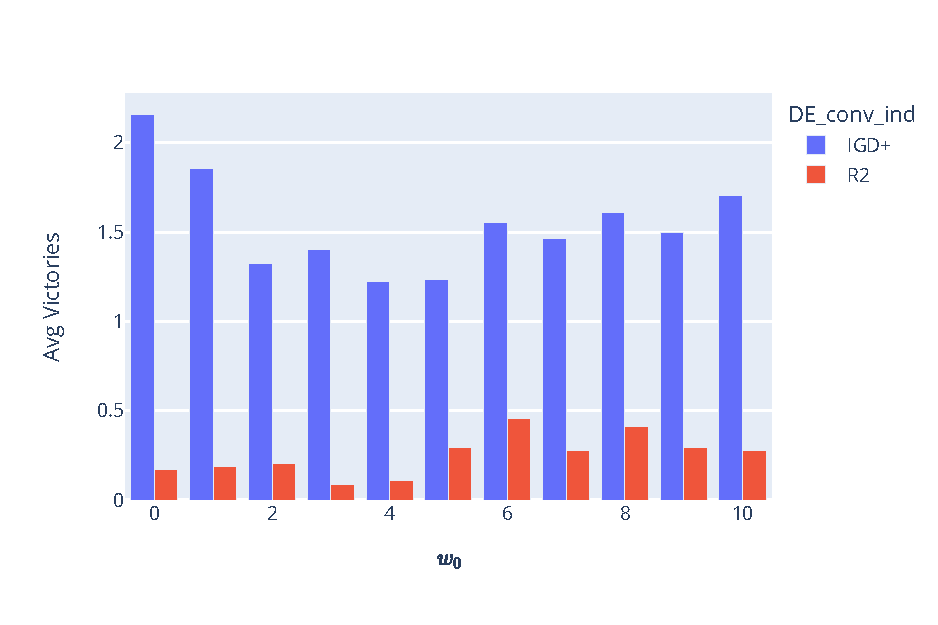
\includegraphics[width=\textwidth]{Figuras/borda_obj_7.pdf}
    \caption[Conteo de borda por número de objetivos]{Quién gana más, para todos los indicadores, conforme cambiamos el peso, para 7 objetivos.}
    \label{fig:borda_obj_7}
\end{figure}


Es importante destacar las diferencias en escala de los dos algoritmos. Claramente en todas las Figuras \ref{fig:borda_obj_2}, \ref{fig:borda_obj_3}, \ref{fig:borda_obj_4}, \ref{fig:borda_obj_5}, \ref{fig:borda_obj_6} y  \ref{fig:borda_obj_7} hay menos proporción de victorias del algoritmo de R2 y parecen no seguir ningún patrón para algún numero de objetivos. Así, la discusión que sigue se hace tomando en cuenta sólo a los valores del algoritmo de IGD+. 
Parece haber una preferencia para $w_0$ grande en dimensiones 3 a 5, notamos como las victorias van ascendiendo de forma monótona conforme le damos más peso a el IGD+ sobre la energía S. Sin embargo, para 2,6 y 7 no es tan claro que es mejor darle prioridad al indicador IGD+. Esto parece ir en contra de lo dicho en \cite{PFI} donde se escogió un $w_0$ mayor para mayores dimensiones bajo el suspuesto de que el indicador de diversidad podría provocar que se estancara la convergencia de la aproximación. Sin embargo, como hemos agrupado todos los indicadores esto también podría ser efecto de que los indicadores de diversidad tienden a ganar más conforme aumentamos los objetivos. Para explorar las consecuencias de este párrafo miraremos ahora una agregaciones por indicadores.

\subsection{Agregación por Indicador}

A continuación se realiza un promedio, por indicador, sobre todos los problemas de los conteos de borda para diferentes combinaciones de pesos. Para aclarar la discusión se dividirá en dos partes; en una se hablarán de los indicadores de convergencia, es decir, que tan bien converge. 



\subsection*{Conteos de Borda para Indicadores de Convergencia}

\begin{figure} [H]
    \centering
    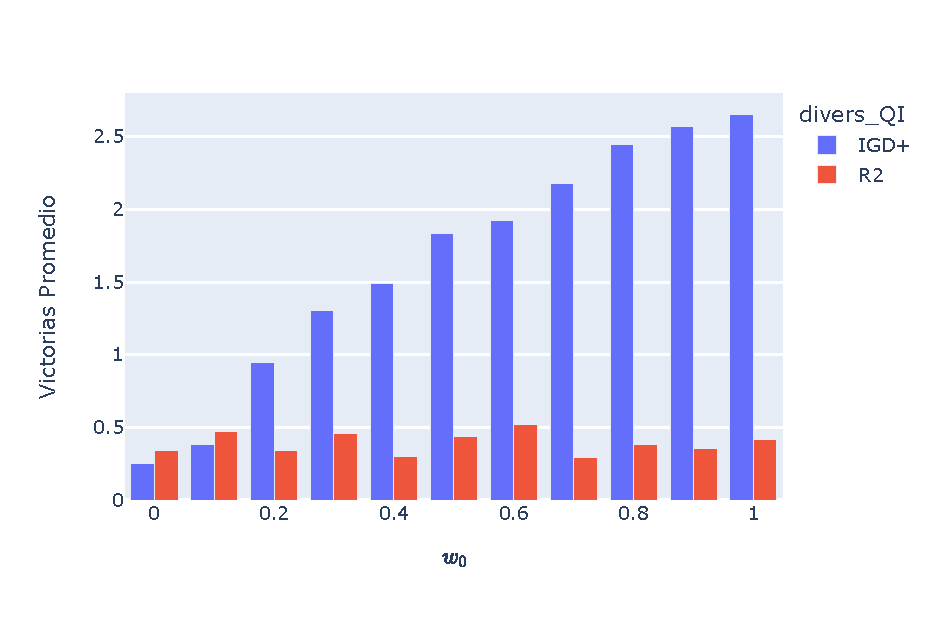
\includegraphics[width=\textwidth]{Figuras/borda_obj_ind_hv.pdf}
    \caption[Conteo de borda HV]{Victorias promedio por problema usando al indicador \textbf{HV} conforme cambiamos los pesos de $w_0$ para todas las dimensiones.}
    \label{fig:borda_hv}
\end{figure}

\begin{figure} [H]
    \centering
    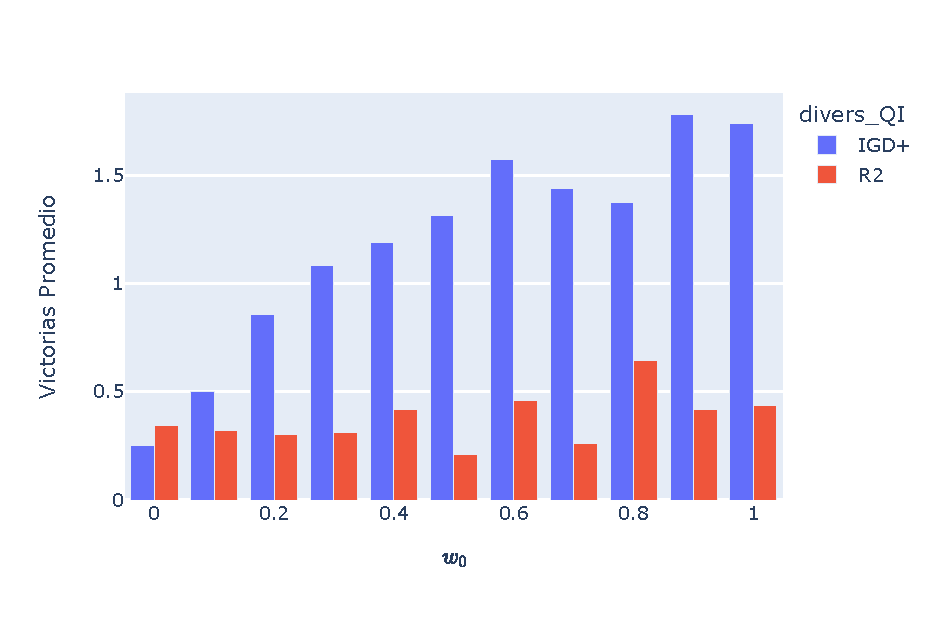
\includegraphics[width=\textwidth]{Figuras/borda_obj_ind_eps+.pdf}
    \caption[Conteo de borda Epsilon +]{Victorias promedio por problema usando al indicador \textbf{$\epsilon +$} conforme cambiamos los pesos de $w_0$ para todas las dimensiones.}
    \label{fig:borda_epsp}
\end{figure}

\begin{figure} [H]
    \centering
    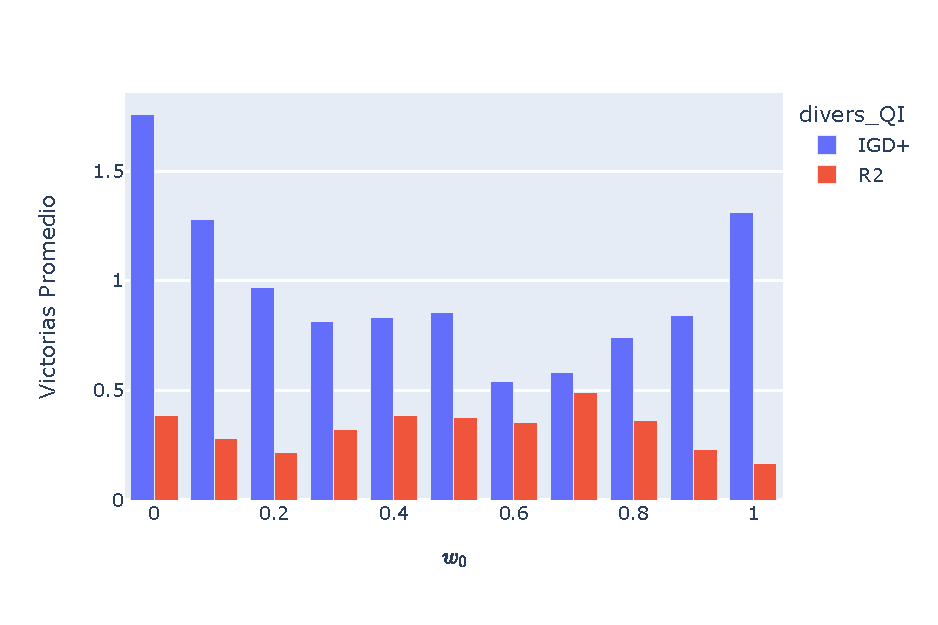
\includegraphics[width=\textwidth]{Figuras/borda_obj_ind_r2.pdf}
\caption[Conteo de borda R2]{Victorias promedio por problema usando al indicador \textbf{R2} conforme cambiamos los pesos de $w_0$ para todas las dimensiones.}
\label{fig:borda_R2}
\end{figure}

Vemos de las Figuras \ref{fig:borda_hv}, \ref{fig:borda_epsp} y \ref{fig:borda_R2} que los indicadores de convergencia que no son R2 tienen un comportamiento monotónico hacia mayores pesos de $w_0$. Es decir, al darle más peso al indicador de convergencia (ya sea IGD+ o R2) en la escalarización de Tchebycheff (Ecuación \ref{eq:ATCH}) obtenemos mayores victorias significativas. No podemos dar una conclusión satisfactoria acerca de porqué R2 tiene este comportamiento.

Ahora miraremos los de convergencia que usan un conjunto de referencia de Pareto, es decir IGD e IGD+. 

\begin{figure} [H]
    \centering
\includegraphics[width=\textwidth]{Figuras/borda_obj_ind_igd.pdf}
\caption[Conteo de borda IGD]{Victorias promedio por problema usando al indicador \textbf{IGD} conforme cambiamos los pesos de $w_0$ para todas las dimensiones.}
\label{fig:borda_igd}
\end{figure}

\begin{figure} [H]
    \centering
\includegraphics[width=\textwidth]{Figuras/borda_obj_ind_igd+.pdf}
\caption[Conteo de borda IGD+]{Victorias promedio por problema usando al indicador \textbf{IGD+} conforme cambiamos los pesos de $w_0$ para todas las dimensiones.}
\label{fig:borda_igdp}
\end{figure}

En el caso de IGD, vemos en la Figura \ref{fig:borda_igd} que no se observa un comportamiento monotónico de la misma forma que con R2. Para IGD+, esto se observa en la Figura \ref{fig:borda_igdp} esto se podría deber a que el indicador no es consistente de Pareto (definido en la Ecuación \ref{eq:consistente_Pareto}).


\subsection*{Conteos de Borda para Indicadores de Diversidad}

\begin{figure} [H]
    \centering
    \includegraphics[width=\textwidth]{Figuras/borda_obj_ind_s-energy.pdf}
    \caption[Conteo de borda IGD+]{Victorias promedio por problema usando al indicador de \textbf{S-Energy} conforme cambiamos los pesos de $w_0$ para todas las dimensiones.}
    \label{fig:borda_senergy}
\end{figure}

\begin{figure} [H]
    \centering
    \includegraphics[width=\textwidth]{Figuras/borda_obj_ind_spd.pdf}
\caption[Conteo de borda IGD+]{Victorias promedio por problema usando al indicador \textbf{SPD} conforme cambiamos los pesos de $w_0$ para todas las dimensiones.}
\label{fig:borda_spd}
\end{figure}



Para los indicadores de diversidad, en las Figuras \ref{fig:borda_senergy} y \ref{fig:borda_spd}, vemos que tenemos el comportamiento esperado para SPD, es decir, decrece el número de victorias de forma monótona conforme aumentamos el peso al indicador de convergencia. Sin embargo, la energía S parece tener un comportamiento opuesto al que esperaríamos, siguiendo más bien a los indicadores de convergencia. Este resultado es muy extraño ya que el algoritmo prioriza menos el indicador de SPD mientras más aumentamos $w_0$. Es decir, parece que para mejorar la Energía S de nuestra aproximación final, no podríamos enfocarnos en mejorarla paso a paso. No podemos dar una explicación satisfactoria de porqué ocurre, pero sería interesante investigarlo en un trabajo futuro.

% \begin{itemize}
%     \item Mostrar diferentes visualizaciones
%     \item Tablas de cada uno de los valores de pesos. Con medias, desviaciones estándar y cuál es mejor según Wilcoxon.
%     \item Boxplots representando lo de las Tablas.
%     \item Gráfico de convergencia (número de evaluaciones (mediana) de función x, valor del indicador en esa generación y): para cada problema hay uno y por cada problema hay una línea de cada combinación de indicadores.
%     \item Conteos de borda para los rankings para ver el ganador.
%     \item Ejemplos de frentes (mediana de la última generación) para más dimensiones PCP. Proyecciones tal vez de casos interesantes. 
%     \item En el apéndice irían todos.   
% \end{itemize}




% \begin{table}[H]
%     \centering
%     \begin{tabular}{|c|c|c|c|}
%     \textbf{Problema} & \textbf{Variables objetivo} & \textbf{Variables decisión} & \textbf{Características PF}                                                                                                 \\ \hline
%     WFG1              & 2,3,4,5,6,7                 & 24,26,28,30,32,34           & \begin{tabular}[c]{@{}c@{}}separable, unifrontal \\ $f_{n_var}$ convexo, el resto mixto\end{tabular}                        \\
%     WFG2              & 2,3,4,5,6,7                 & 24,26,28,30,32,34           & \begin{tabular}[c]{@{}c@{}}No separable.\\ $f_{n_var}$ unimodal, el resto multimodal.\\ Convexo, desconectado.\end{tabular} \\
%     WFG3              & 2,3,4,5,6,7                 & 24,26,28,30,32,34           & \begin{tabular}[c]{@{}c@{}}No separable. Unifrontal.\\ Lineal, degenerado\end{tabular}                                      \\
%     WFG4              & 2,3,4,5,6,7                 & 24,26,28,30,32,34           & Separable. Multifrontal. Cóncavo.                                                                                           \\
%     WFG5              & 2,3,4,5,6,7                 & 24,26,28,30,32,34           & Separable. Deceptivo. Cóncavo.                                                                                              \\
%     WFG6              & 2,3,4,5,6,7                 & 24,26,28,30,32,34           & No separable. Unifrontal.Cóncavo.                                                                                           \\
%     WFG7              & 2,3,4,5,6,7                 & 24,26,28,30,32,34           & Separable. Unifrontal.Cóncavo.                                                                                              \\
%     WFG8              & 2,3,4,5,6,7                 & 24,26,28,30,32,34           & No separable,Unifrontal. Cóncavo                                                                                            \\
%     WFG9              & 2,3,4,5,6,7                 & 24,26,28,30,32,34           & \begin{tabular}[c]{@{}c@{}}No separable. Multifrontal, deceptivo.\\ Cóncavo\end{tabular}                                   
%     \end{tabular}
% \end{table}
% \begin{table}[H]
%     \centering
%     \begin{tabular}{|c|c|c|c|}
%     \textbf{Problema} & \textbf{Variables objetivo} & \textbf{Variables decisión} & \textbf{Características PF}                                                                                                                                   \\ \hline
%     DTLZ1             & 2,3,4,5,6,7                 & 6,7,8,9,10,11               & separable, multifrontal, lineal                                                                                                                               \\
%     DTLZ2             & 2,3,4,5,6,7                 & 12,13,14,15,16              & separable, unifrontal, cóncavo                                                                                                                                \\
%     DTLZ3             & 2,3,4,5,6,7                 & 12,13,14,15,16              & separable, multifrontal, cóncavo                                                                                                                              \\
%     DTLZ4             & 2,3,4,5,6,7                 & 12,13,14,15,16              & separable, unifrontal, cóncavo                                                                                                                                \\
%     DTLZ5             & 2,3,4,5,6,7                 & 12,13,14,15,16              & \begin{tabular}[c]{@{}c@{}}unifrontal, \\ degenerado\end{tabular}                                                                                             \\
%     DTLZ6             & 2,3,4,5,6,7                 & 12,13,14,15,16              & unifrontal, degenerado                                                                                                                                        \\
%     DTLZ7             & 2,3,4,5,6,7                 & 21,22,23,24,25,26           & \begin{tabular}[c]{@{}c@{}}$f_{n_var}$ separable, para el resto no aplica\\ $f_{n_var}$ unimodal, para el resto multimodal\\ desconectado, mixto\end{tabular}
%     \end{tabular}
%     \caption[Problemas prueba usados ]{Problemas pruebas usados así como sus variables objetivo, de decisión,  y algunas características de su frente de Pareto.}
%     \label{Tabla:problema_prueba}
% \end{table}
   % ~20 páginas - Presentar los resultados tal cual son, y analizarlos.
\chapter{Discusión de Resultados}
% \blindtext

En este capítulo intentaremos dar respuesta a las preguntas planteadas en la introducción con base a lo visto en los capítulos anteriores.

\subsection*{¿Existe una diferencia en el desempeño del algoritmo PFI-EMOA al variar la combinación los pesos?}

Claramente si existe una diferencia, como podemos ver en las Figuras \ref{fig:KW_dim_IGDp}, \ref{fig:KW_dim_R2}, \ref{fig:KW_conv_dist_IGDp} y \ref{fig:KW_conv_dist_R2}, . También notamos en estas Figuras que la elección del indicador de convergencia del algoritmo PFI-EMOA importa mucho para la sensibilidad con respecto a la combinación de pesos. En particular, R2 es mucho menos sensible que IGD+. Este resultado es importante ya que PFI-EMOA demostró ser mejor que muchos EMOAs  y en este trabajo hemos mostrado que la elección de los pesos en la escalarización de Tchebycheff sí importa. Sobre todo metiéndonos más en detalles acerca de la aproximación final, es decir, si el DM quisiera una solución con mayor SPD sabríamos que tenemos que una buena heurística sería darle mayor peso a los primero valores. 

\subsection*{¿Qué combinación de pesos es mejor para cada problema?}

Usando las agregaciones mostradas en el capítulo anterior en las Figuras \ref{fig:borda_obj_2}, \ref{fig:borda_obj_3}, \ref{fig:borda_obj_4}, \ref{fig:borda_obj_5}, \ref{fig:borda_obj_6} y \ref{fig:borda_obj_7} podemos tener una idea que el número de objetivos del problema si afecta a la elección de pesos. En particular el hecho de que para dos dimensiones parezca no importar indica que tal vez los objetivos de ambos indicadores están alineados hasta cierto punto y parece suceder lo mismo cuando los objetivos se vuelven mayores que 5. Agrupando sobre la categoría de los indicadores notamos de las Figuras \ref{fig:borda_hv}, \ref{fig:borda_epsp}, \ref{fig:borda_R2}, \ref{fig:borda_igd} y \ref{fig:borda_igdp}  que los indicadores de convergencia que son consistentes de Pareto si crecen conforme le damos más importancia a IGD+, teniendo nuevamente resultados aparentemente sin patrones tan claros cuando usamos R2 en el estimador de densidad. Los indicadores de diversidad que se muestran en la Figura \ref{fig:borda_senergy}, \ref{fig:borda_spd} también siguen un comportamiento casi monotónico con el peso de $w_0$ para el caso de IGD+, es decir, mientras más peso le damos al indicador de diversidad, obtenemos una solución más diversa. 

Nuevamente no encontramos ningún comportamiento notorio en los resultados del algoritmo que usa a R2. Es importante notar que no necesariamente se le da más importancia a uno u a otro indicador siempre. Sino que, como se explica en la Sección \ref{sec:PFI-EMOA}, el algoritmo entra a la parte del estimador de densidad cuando no encuentra más de una solución que contribuye lo mismo para cambiar el indicador de IGD+ (como se puede ver en la línea 6 de el Algoritmo \ref{alg:PFI-EMOA}). Entonces, el efecto que tengan los diferentes pesos también se verá afectado con cuántas veces sea esta situación relevante. Así, podría pasar que es importante para algún algoritmo priorizar más un indicador, sin embargo, no se le da la oportunidad de tener un efecto tan grande.  


\subsection*{¿Qué sucede cuando cambiamos el indicador de convergencia de IGD$+$ a R2?}

Aunque ya hemos visto que hay menos sensibilidad a los pesos por parte del indicador R2, en esta sección miraremos esto con mayor detalle, haciendo las comparaciones de algoritmos directamente entre IGD+ y R2. Por ejemplo, para hacer el análisis de las Figuras \ref{fig:R2_vs_IGDp_2}, \ref{fig:R2_vs_IGDp_3}, \ref{fig:R2_vs_IGDp_4}, \ref{fig:R2_vs_IGDp_5}, \ref{fig:R2_vs_IGDp_6} y \ref{fig:R2_vs_IGDp_7}, para cada configuración de pesos, se tomaron los algoritmos de IGD+ y R2 y se compararon usando Wilcoxon, así se promediaron 11 comparaciones para ver en cuál ganaba cierto algoritmo. Cabe destacar que para este caso se tuvo que cambiar el signo de los indicadores que se tienen que minimizar para poder usar la prueba de Wilcoxon y ver si el algoritmo de IGD+ era mayor al algoritmo de R2 o viceversa.


\begin{figure} [H]
    \centering
\includegraphics[width=\textwidth]{Figuras/R2_vs_IGDp_nobj2.pdf}
\caption[IGD+ vs R2 2 objetivos]{Porcentaje de victorias de diferentes indicadores de convergencia en la escalarización de Tchebycheff para 2 objetivos.}
\label{fig:R2_vs_IGDp_2}
\end{figure}

\begin{figure} [H]
    \centering
\includegraphics[width=\textwidth]{Figuras/R2_vs_IGDp_nobj3.pdf}
\caption[IGD+ vs R2 3 objetivos]{Porcentaje de victorias de diferentes indicadores de convergencia en la escalarización de Tchebycheff para 3 objetivos.}
\label{fig:R2_vs_IGDp_3}
\end{figure}

\begin{figure} [H]
    \centering
\includegraphics[width=\textwidth]{Figuras/R2_vs_IGDp_nobj4.pdf}
\caption[IGD+ vs R2 4 objetivos]{Porcentaje de victorias de diferentes indicadores de convergencia en la escalarización de Tchebycheff para 4 objetivos.}
\label{fig:R2_vs_IGDp_4}
\end{figure}

\begin{figure} [H]
    \centering
\includegraphics[width=\textwidth]{Figuras/R2_vs_IGDp_nobj5.pdf}
\caption[IGD+ vs R2 5 objetivos]{Porcentaje de victorias de diferentes indicadores de convergencia en la escalarización de Tchebycheff para 5 objetivos.}
\label{fig:R2_vs_IGDp_5}
\end{figure}

\begin{figure} [H]
    \centering
\includegraphics[width=\textwidth]{Figuras/R2_vs_IGDp_nobj6.pdf}
\caption[IGD+ vs R2 6 objetivos]{Porcentaje de victorias de diferentes indicadores de convergencia en la escalarización de Tchebycheff para 6 objetivos.}
\label{fig:R2_vs_IGDp_6}
\end{figure}

\begin{figure} [H]
    \centering
\includegraphics[width=\textwidth]{Figuras/R2_vs_IGDp_nobj7.pdf}
\caption[IGD+ vs R2 7 objetivos]{Porcentaje de victorias de diferentes indicadores de convergencia en la escalarización de Tchebycheff para 7 objetivos.}
\label{fig:R2_vs_IGDp_7}
\end{figure}

De las Figuras \ref{fig:R2_vs_IGDp_2}, \ref{fig:R2_vs_IGDp_3}, \ref{fig:R2_vs_IGDp_4}, \ref{fig:R2_vs_IGDp_5}, \ref{fig:R2_vs_IGDp_6} y \ref{fig:R2_vs_IGDp_7}  podemos ver con una comparación directa que los algoritmos de IGD+ tienden a tener mejor desempeño que los de IGD. Teniendo excepciones para 5 objetivos, como podemos ver en la Figura \ref{fig:R2_vs_IGDp_5}, en los indicadores IGD+ y R2, donde el algoritmo de R2 tiene mejor desempeño en promedio. No podemos concluir porqué es que esto ocurre sólo para este caso, pero es un buen problema para trabajo futuro.

Un resultado interesante de estas últimas gráficas es que, aunque R2 no es tan sensible a cambiar su desempeño conforme se cambia $w_0$, su desempeño se vuelve mejor conforme subimos las dimensiones. Habiendo casos donde aunque no haya mucha diferencia entre los diferentes pesos para R2, tiene mejor desempeño que IGD+. En 2 y 3 dimensiones los resultados están muy dominados por IGD+. 

También hacemos las comparaciones análogas a las hechas para diferente número de objetivos, pero con el tipo del indicador y presentamos los resultados en la Figura \ref{fig:R2_IGDp_cat}.


\begin{figure}[H]
    \centering
    \includegraphics[width=\textwidth]{Figuras/R2_vs_IGDp_por_tipo_ind.pdf}
    \caption[R2 vs IGD+, victorias por indicador.]{Comparaciones de victorias de cada algoritmo para cada $w_0$ tomando en cuenta el tipo de indicador que se está optimizando.}
    \label{fig:R2_IGDp_cat}
\end{figure}


Vemos que IGD+ gana más veces que R2 sin embargo para los indicadores de convergencia hay más casos donde no se puede concluir que no se rechaza la hipótesis nula de una distribución simétrica alrededor del 0. En los indicadores de diversidad existe mucha preferencia por los de IGD+. Lo que nos podría hablar de preferir este tipo de algoritmos sobte los de R2 cuando se realice este análisis. 


Finalmente, en la Figura \ref{fig:R2_IGDp}, presentamos el análisis con mayor agrupación en el que comparamos directamente los algoritmos de R2 e IGD+ a través de todos los pesos, pareando las diferentes combinaciones de pesos, pero sin hacer ninguna otra división. 


\begin{figure}[H]
    \centering
    \includegraphics[scale=.7]{Figuras/R2_vs_IGDp.pdf}
    \caption[Victorias por algoritmo]{Victorias de cada algoritmo. El restante del $100\%$ son en las que no se rechazó la hipótesis nula.}
    \label{fig:R2_IGDp}
\end{figure}


Una vez más vemos que IGD+ tiene un mejor desempeño que R2 en el agregado, sin embargo, el detalle es importante para escoger que usar en cada problema. 

Habiendo presentado una breve discusión de los resultados, en el capítulo siguiente daremos ideas de cómo mejorar y hacer más formales estos resultados. 



            % ~5 páginas - Resumir lo que se hizo y lo que no y comentar trabajos futuros sobre el tema
\chapter{Conclusiones y Trabajo Futuro}

En el capítulo anterior revisamos la respuesta a tres de las preguntas que nos propusimos contestar cuando empezamos este trabajo. En este capítulo veremos las dos restantes, hablando de las dificultades de resolverlas y como se podrían abordar en un trabajo futuro. También se habla de las conclusiones del trabajo en general.


\section{Conclusiones}

% Qué se hizo

En este trabajo se probaron diferentes combinaciones de parámetros para el Algoritmo PFI-EMOA \cite{PFI}. Los parámetros controlan que tanta importancia le damos a indicadores de convergencia (R2, IGD+) o a indicadores de diversidad (Energía-S). Como estos indicadores tienen metas distintas es interesante ver cuál es el efecto de cambiarlas.

% Qué experimentos
El valor de los parámetros se cambió de manera sistemática, para comparar cuando un algoritmo tiene un desempeño distinto de manera estadísticamente significativa. El desempeño se comparó a través de indicadores de calidad en distintas categorías, como vimos en el capítulo anterior. Además de esto, se modificó el indicador de convergencia usado en \cite{PFI} en el estimador de densidad, el original es IGD+ y se hicieron los mismos experimentos con el indicador de R2. 

Se realizaron 10 experimentos con una semilla aleatoria distinta para cada una de las combinaciones de parámetros (los detalles de la semilla usada están en el Apéndice \ref{sec:Apendice_semilla}). Después se caracterizó que tan buena fue la solución obteniendo el Hipervolumen, R2, IGD, IGD+, $\epsilon +$, Energía-S y SPD. Así, se obtuvieron 10 mediciones de cada uno de estos indicadores por cada combinación de pesos en la escalarización de Tchebycheff. 

Para medir las diferencias entre estas poblaciones de indicadores se usaron dos pruebas estadísticas. La primera que se realizó fue la de Friedman que nos indica si hay una diferencia significativa entre alguna combinación de parámetros. También se usó la prueba de Wilcoxon para ver en qué caso un indicador es mejor que otro. Hay que tener en cuenta que hay unos indicadores que se vuelven mejores al maximizarse y algunos se vuelven mejores al minimizarse.  

% Hallazgos más importantes
Se observan diferencias significativas en todos estos casos. Teniendo los indicadores de convergencia una preferencia por mayor peso a la parte de IGD+ o R2 en el estimador de densidad. Esto tiene sentido aunque a veces encontramos resultados que parecen indicar que para optimizar un indicador en el conjunto de aproximación final, no basta con optimizarlo paso con paso (como haría un algoritmo voraz). Sino que por el contrario, darle un peso mayor a un indicador de convergencia como Energía-S resultará en un desempeño mejor.

Al cambiar el indicador de convergencia con el que se define el estimador de densidad del algoritmo de PFI-EMOA \cite{PFI} de IGD+ a R2 vemos que IGD+ obtiene mucho mejores resultados, como se puede observar en la Figura \ref{fig:R2_IGDp}.

Cuando se mira el efecto que tiene cambiar el peso de la escalarización de Tchebycheff en el indicador de diversidad de la aproximación al frente de Pareto obtenemos resultados contrastantes. Por un lado, en la Figura \ref{fig:borda_spd}, vemos que al darle más peso a Energía-S obtenemos un mejor desempeño en SPD. Sin embargo, al revisar Energía-S en la Figura \ref{fig:borda_senergy}, vemos que cuando le damos más importancia al indicador de convergencia obtenemos menos victorias.

\section{Trabajo Futuro}
\section*{¿Qué tipo de problemas prefieren ciertas combinaciones?}
Esta respuesta sólo se pudo dar de manera descriptiva, a través de visualizaciones. Sin embargo, un análisis más detallado tendría que tomar en cuenta, no sólo los patrones que nos son visibles a través de gráficas de comportamiento, sino a las características mismas del problema a resolver. Este tipo de problemas, donde se intenta dar una predicción hacia los mejores parámetros que solucionarían un problema con ciertas características, caen dentro de la rama de estudio llamada Exploratory Landscape Analysis o ELA por sus siglas en inglés \cite{trajanovExplainableLandscapeAnalysis2022}. La implementación de estos métodos puede usarse para automatizar la selección de algoritmos dados algunos problemas con ciertas características y un muestreo de los resultados que se obtienen al escoger algunos problemas. En nuestro problema los parámetros a escoger incluirían características de la población, es decir, indicadores de calidad; el número de objetivos del problema, la forma del frente de Pareto (podemos ver en la Tabla \ref{Tabla:QIs}), el peso de la combinación de Tchebycheff usado para guiar el proceso de búsqueda y el indicador a optimizar. 

Se entrena un modelo de aprendizaje de máquina como un árbol de decisión para poder realizar la selección de algoritmo. Así, podríamos conocer a priori que modelo usar para obtener un resultado que busquemos o que coincida con las preferencias del tomador de decisiones. 

Este enfoque sería para ajustar los parámetros desde el inicio del problema y esperar los resultados, sin embargo, también podría ser usado para cambiar los parámetros momento a momento como explicamos en la siguiente sección. 

\section*{¿Se puede ir cambiando este algoritmo paso a paso?}

En este trabajo se fijó la combinación de indicadores desde el inicio y después se dejó ejecutar el algoritmo hasta alcanzar su condición de paro (detallado en el Algoritmo \ref{alg:PFI-EMOA}). Sin embargo, la combinación de pesos no tiene porqué ser estática. Encontrar nuevas situaciones puede llevar a que algún indicador cambie de importancia. Por ejemplo, si se estanca la convergencia se le puede dar más valor al indicador de IGD+ o inclusive cambiar el estimador de densidad para que sea, en vez de IGD+, R2 o cualquier otro indicador. Inclusive se puede cambiar la escalarización de Tchebycheff o el criterio de selección de población. Las decisiones acerca de cómo cambiar el algoritmo podrían estar informadas por los resultados de los modelos de ELA que se entrenen con todo un dataset de problemas como se explicó en la pregunta anterior. Así podríamos ir adaptándonos al problema en vez de sólo esperar a que la ejecución se acabe para saber si la elección de parámetros fue correcta.

Por otro lado, es posible también usar  Aprendizaje por Refuerzo \cite{Sutton1998} para guiar la búsqueda de mejores aproximaciones al frente de Pareto. Aprendizaje por Refuerzo es una rama de la inteligencia artificial en la que se entrena a un agente para aprender qué hacer con base en una función de recompensa dada paso a paso. Es decir, se aprende la mejor manera de tomar una serie de acciones (política) dada una función de recompensa que recibe el agente con cada una de sus acciones. Esto difiere del aprendizaje supervisado en el sentido de que la función a maximizar en este último caso suele ser fija y conocida. Los métodos de solución de Aprendizaje por Refuerzo permiten inicializar un agente con una política aleatoria e ir aprendiendo una mejor política conforme vamos entrenando el modelo. El agente no necesita saber los detalles del problema antes de comenzar a entrenarse. De modo que el agente podría iniciar en una política de elección de pesos para el problema y basándose en su estado de cada iteración del problema tomar una acción de cómo modificar este peso para encontrar una solución que vaya más de acuerdo con las preferencias del tomador de decisiones. El estado estaría descrito por las características poblacionales (indicadores de calidad) así como las preferencias del DM, cualquier información que se tenga sobre el frente de Pareto del problema, etc. 



            % ~5 páginas - Resumir lo que se hizo y lo que no y comentar trabajos futuros sobre el tema


%%%%%%%%%%%%%%%%%%%%%%%%%%%%%%%%%%%%%%%%%%%%%%%%%%%%%
%                   APÉNDICES                       %
%%%%%%%%%%%%%%%%%%%%%%%%%%%%%%%%%%%%%%%%%%%%%%%%%%%%%
\appendix
% this file is called up by thesis.tex
% content in this file will be fed into the main document
\chapter{Resultados de todos los experimentos}
% top level followed by section, subsection
\section{Semillas usadas en los experimentos} \label{sec:Apendice_semilla}
Con el fin de garantizar la reproducibilidad de los experimentos se usaron las siguientes semillas para las inicialización de las poblaciones en cada una de las 10 diferentes ejecuciones por cada combinación de peso 

\begin{figure}[H]
\centering
\begin{lstlisting}[caption=inicio del programa seed.dat que contiene a las semillas usadas]
    # seed.dat
    #
    # List of prime numbers employed as seeds for the random number generator
    # Numbers must have less than or equal to 7 digits (float numbers)
    #
    # List retrieved from:
    # http://www.bigprimes.net/archive/prime/1001/
    # https://primes.utm.edu/lists/small/millions/
    #
    5
    13
    23
    37
    47
    61
    73
    89
    103
    113
\end{lstlisting}
\end{figure}

% \section{Tablas}
% \section{Boxplots}
% \section{Heatmaps}


               % Colocar los circuitos, manuales, código fuente, pruebas de teoremas, etc.

%%%%%%%%%%%%%%%%%%%%%%%%%%%%%%%%%%%%%%%%%%%%%%%%%%%%%
%                   REFERENCIAS                     %
%%%%%%%%%%%%%%%%%%%%%%%%%%%%%%%%%%%%%%%%%%%%%%%%%%%%%
% existen varios estilos de bilbiografía, pueden cambiarlos a placer
\bibliographystyle{unsrt}

% \bibliographystyle{apalike} % otros estilos pueden ser abbrv, acm, alpha, apalike, ieeetr, plain, siam, unsrt

%El formato trae otros estilos, o pueden agregar uno que les guste:
%\bibliographystyle{Latex/Classes/PhDbiblio-case} % title forced lower case
%\bibliographystyle{Latex/Classes/PhDbiblio-bold} % title as in bibtex but bold
%\bibliographystyle{Latex/Classes/PhDbiblio-url} % bold + www link if provided
%\bibliographystyle{Latex/Classes/jmb} % calls style file jmb.bst

\bibliography{Bibliografia/referencias_1}             % Archivo .bib


\end{document}
